\documentclass[
  12pt,			      % tamanho da fonte
  openright,		      % capítulos começam em pág ímpar (insere página vazia caso preciso)
  oneside,			  % para impressão em recto e verso. Oposto a oneside
  a4paper,			  % tamanho do papel. 
  chapter=TITLE,        % títulos de capítulos convertidos em letras maiúsculas
  section=TITLE,        % títulos de seções convertidos em letras maiúsculas
  english,			  % idioma adicional para hifenização
  french,				  % idioma adicional para hifenização
  spanish,			  % idioma adicional para hifenização
  brazil				  % o último idioma é o principal do documento
]{iftex}

% Importa as macros do projeto
%% Macros de dados do documento
\autor{Henrique Machado de Oliveira}
% Título PROVISÓRIO (19/11/2026): a versão mais longa em discussão, posta para
% conferir se cabe na capa depois de compilada. Tirou-se "com abordagem
% Teacher-Student" (pseudo-rotulagem já diz o mesmo). As versões enxutas estão
% em docs/Titulo TCC.txt. Escolhido o título, registrar em docs/decisoes.md.
\titulo{ARIA: \textit{Pipeline} Hierárquico de Visão Computacional para Marcação Automatizada de Anomalias por Pseudo-Rotulagem em Chapas de Rochas Ornamentais com Critério Parametrizado por Litologia}
%%%Título anterior: Redes Neurais Convolucionais para o Controle de Qualidade de Rochas Ornamentais: Da Classificação à Segmentação de Anomalias utilizando pipeline com abordagem Teacher-Student

%%%Sistema Hierárquico de Inteligência Artificial para o Controle de Qualidade de Rochas Ornamentais: Da Classificação à Segmentação de Irregularidades
%%%Análise Comparativa entre Modelos de Segmentação Generalistas e Arquiteturas em Cascata para Identificação de Defeitos em Rochas Ornamentais
%%%Otimização da Segmentação de Superfícies Pétreas através de Classificação Prévia e Redes Especialistas
%%%Abordagem Hierárquica em Deep Learning: Impacto da Especialização de Modelos na Precisão da Segmentação de Rochas Ornamentais

\instituicao{Instituto Federal do Espírito Santo}
\curso{Bacharelado em Sistemas de Informação}
\local{Cachoeiro de Itapemirim}
\data{2026}
\tipotrabalho{Trabalho de Graduação}
\preambulo{Trabalho de Conclusão de Curso apresentado à Coordenadoria do Curso de Sistemas de Informação do Instituto Federal de Educação, Ciência e Tecnologia do Espírito Santo, como requisito parcial para a obtenção do título de Bacharel em Sistemas de Informação.}

\orientador[Orientador][Prof. Dr.]{Rafael}[Silva Guimarães]{Instituto Federal do Espírito Santo}
%%%\coorientador[Coorientador][Prof. Dr.]{Everson}[Scherrer Borges]{Instituto Federal do Espírito Santo}
%%%\coorientador[Coorientador][Prof. Dr.]{Igor}[Henrique Beloti Pizetta]{Instituto Federal do Espírito Santo}

\examinadori{Profa. Dra. Fulana de Tal}{Instituto Federal do Espírito Santo}{Examinadora}
\examinadorii{Prof. Dr. Cicrano de Tal}{Instituto Federal do Espírito Santo}{Examinador}

% TODO: data real da defesa, a confirmar com o orientador (ver docs/pendencias.md).
\approvaldate{15}{Outubro}{2026}

% Palavras-chaves
\palavraschave{Visão Computacional}[Segmentação Semântica][Rochas Ornamentais][Modelos de Fundação][Pseudo-rotulagem]
\keywords{Computer Vision}[Semantic Segmentation][Dimension Stone][Foundation Models][Pseudo-labeling]

% Ficha catalográfica
\fichabiblioteca{
    Dados Internacionais de Catalogação-na-Publicação (CIP) \\
    (Biblioteca Nilo Peçanha do Instituto Federal do Espírito Santo)
}
\fichaautor{Elaborada por XXXXXXXXXXXXXXXXXXXXX – CRB-X/ES - XXX}
\fichatags{
    1. Visão computacional.  
    2. Aprendizado profundo.  
    3. Segmentação de imagens.  
    4. Rochas ornamentais – Controle de qualidade.  
    5. Inteligência artificial.  
    I. Guimarães, Rafael Silva.  
    II. Instituto Federal do Espírito Santo.  
    III. Título.
}

\cutter{X999y}
\cdd{000.00}
\selectlanguage{brazil}

% Arial (para usar times-new-roman, comente as três linhas abaixo)
\usepackage{helvet}
\renewcommand{\familydefault}{\sfdefault}
\renewcommand{\ABNTEXchapterfont}{\bfseries}
% Comandos para revisar o texto
\usepackage{easyReview} 


%% Elementos opcionais
\editardedicatoria{A dedicatória é um elemento opcional. Contém o oferecimento do trabalho adeterminada pessoa ou a pessoas (ASSOCIAÇÃO BRASILEIRA DE NORMAS TÉCNICAS, 2011b).}
\editaragradecimentos{Agradeço a Deus, pela fé que me sustentou ao longo do curso e deste trabalho.

À minha família, pelo apoio e pela paciência durante os anos de graduação.

Ao meu orientador, Prof. Dr. Rafael Silva Guimarães, pela orientação e pelo acompanhamento ao longo deste trabalho. Ao Prof. Dr. Everson Scherrer Borges, que orientou a sua primeira etapa.

À Marcelli da Fonseca Carvalho, que aceitou julgar, uma a uma e sem saber de onde vinham, as marcações da auditoria cega, sem obrigação nenhuma de fazê-lo. O trabalho se propôs a medir o critério de marcação contra o julgamento de alguém que não participou da calibração, e esse olhar foi o dela. Obrigado pelo tempo e pela paciência com centenas de recortes de rocha.

Aos colegas de pesquisa com quem construí o DeepStoneAI e o FracStoneAI, trabalhos dos quais o ARIA é continuação: Matheus Gimenes de Souza, Arthur Cesar Figueiredo da Silva, Andrey Magalhães Silva, Pedro Brito Moreira, Igor Henrique Beloti Pizetta e Juliano Tessinari Zagôto. A João Victor Costa Araujo, por ter tornado público o conjunto de imagens sem o qual este trabalho não existiria.

Ao Instituto Federal do Espírito Santo, Campus Cachoeiro de Itapemirim, e aos professores do curso de Sistemas de Informação, pela formação.

Ao Sesi Cachoeiro e aos professores que me incentivaram a escolher este curso e com quem aprendi muito.

Aos colegas próximos do Ifes, pela convivência e pela companhia ao longo do curso.
}
\editarepigrafe{\begin{minipage}{.8\textwidth}
\raggedleft
\textit{``Essentially, all models are wrong, but some are useful.''}

\vspace{0.5cm}
George E. P. Box e Norman R. Draper, \textit{Empirical Model-Building and Response Surfaces} (1987)
\end{minipage}
}


%% Listas [Siglas e Simbolos]
\editarlistasiglas{\begin{siglas}
    \item[AP] Precisão Média (\textit{Average Precision})
    \item[ARIA] Análise e Reconhecimento Inteligente de Anomalias
    \item[CLIP] \textit{Contrastive Language--Image Pre-training}
    \item[CNN] Rede Neural Convolucional (\textit{Convolutional Neural Network})
    \item[FN] Falso Negativo
    \item[FP] Falso Positivo
    \item[GPU] Unidade de Processamento Gráfico (\textit{Graphics Processing Unit})
    \item[Ifes] Instituto Federal do Espírito Santo
    \item[IoU] \textit{Intersection over Union}
    \item[mAP] \textit{mean Average Precision}
    \item[NMS] Supressão de Não-Máximos (\textit{Non-Maximum Suppression})
    \item[SAM] \textit{Segment Anything Model}
    \item[VP] Verdadeiro Positivo
    \item[YOLO] \textit{You Only Look Once}
\end{siglas}
}
\editarlistasimbolos{\begin{simbolos}
    \item[$\lambda$] Letra grega labda
\end{simbolos}}

% Novos comandos
\newcommand{\ie}{\textit{i.e. }}
\newcommand{\eg}{\textit{e.g. }}

\begin{document}

  % --------------------------------------------------- %
  % CAPAS                                               %
  % --------------------------------------------------- %
  % CAPA E FOLHA DE ROSTO
  \capas
  \imprimircapa
  \imprimirfolhaderosto
  % A ficha catalográfica é feita pela biblioteca do Ifes depois da defesa; a
  % versão gerada pelo template só imprimia os campos "XXXX" de macros.tex.
  % Quando a biblioteca devolver a ficha oficial em PDF, descomente:
  % \includepdf[pages=-]{pre_textuais/ficha.pdf}
  %%%\imprimirfichacatalografica

  % --------------------------------------------------- %
  % ELEMENTOS PRÉ-TEXTUAIS                              %
  % --------------------------------------------------- %
  % APROVAÇÃO, DEDICATÓRIA, AGRADECIMENTOS, EPÍGRAFE
  \pretextual
  % Banca definida em macros.tex (Henrique, 24/11/2026). Falta a data da defesa
  % (\approvaldate em macros.tex); descomente a aprovação quando ela vier.
  %%%\imprimiraprovacao
  % \includepdf[pages=-]{pre_textuais/aprovacao.pdf}
  % Dedicatória: sem, por enquanto (Henrique, 23/11/2026).
  %%%\imprimirdedicatoria
  \imprimiragradecimentos
  \imprimirepigrafe
  
  % RESUMO - PT/EN
  % RESUMO - PT
\begin{resumo}
  \vspace{-15pt}

  A inspeção de anomalias superficiais em chapas de rochas ornamentais é feita visualmente por operadores, e o critério que separa uma feição natural de um defeito comercial não está escrito em lugar nenhum: ele varia com a rocha, o cliente, o lote e o inspetor. Este trabalho parte da premissa de que esse critério é arbitrário por natureza e propõe torná-lo explícito, parametrizado e auditável, em vez de tentar eliminá-lo. Propõe-se o ARIA (Análise e Reconhecimento Inteligente de Anomalias), um \textit{pipeline} hierárquico de visão computacional em que um classificador identifica a litologia da chapa, um modelo de fundação guiado por texto atua como Professor, gerando polígonos de anomalia sem anotação humana, e uma rede de segmentação compacta, a ser treinada sobre esses polígonos, atua como Aluno na linha de produção. Esta versão implementa e avalia os dois primeiros estágios; o treinamento do Aluno é trabalho futuro. Em cada litologia, o critério vira uma lista de termos que descrevem defeitos, as sondas, e, para cada sonda, um nível mínimo de confiança, o limiar, calibrados em quatro imagens; o limiar sai de uma regra automática, a mesma para todas as litologias. O experimento compara quatro configurações do Professor, e a hipótese opõe essa regra aplicada a cada litologia separadamente e a todas juntas. A referência é uma auditoria cega, em que uma avaliadora julga cada marcação sem saber de que configuração ela veio, com o critério de decisão fixado antes dos julgamentos. Nas onze litologias com mais imagens, o autor ajustou o limiar da regra em todos os 45 pares de litologia e sonda, sempre para cima e, em mediana, 3,3 vezes; em sete delas, subiu-o até que a superfície sem defeito da chapa comum deixasse de ser marcada. O classificador de litologias, reproduzido de trabalho anterior, atingiu 96,72\% de acurácia na partição de teste original e 99,92\% com partições sorteadas por imagem.
  % TODO: acrescentar uma frase de resultado do experimento quando a auditoria for julgada.

  Palavras-chave: \palavraschaveemlinha
\end{resumo}


% RESUMO - EN
\begin{resumo}[Abstract]
  \vspace{-15pt}

  \begin{otherlanguage*}{english}
  Surface anomaly inspection of polished dimension stone slabs is performed visually by human operators, and the criterion separating a natural feature from a commercial defect is nowhere written down: it varies with the stone, the customer, the batch and the inspector. This work takes that criterion to be arbitrary by nature and proposes to make it explicit, parameterised and auditable, rather than trying to eliminate it. We propose ARIA, a hierarchical computer vision pipeline in which a classifier identifies the slab lithology, a text-prompted foundation model acts as a Teacher, producing anomaly polygons without human annotation, and a compact segmentation network, to be trained on those polygons, acts as a Student on the production line. This version implements and evaluates the first two stages; training the Student is left as future work. For each lithology, the criterion becomes a list of terms describing defects, the probes, and, for each probe, a minimum confidence level, the threshold, calibrated on four images; the threshold comes from an automatic rule, the same for every lithology. The experiment compares four Teacher configurations, and the hypothesis opposes that rule applied to each lithology separately and to all of them pooled. The reference is a blind audit, in which an evaluator judges each marking without knowing which configuration produced it, with the decision criterion fixed before any judgement. Across the eleven lithologies with the most images, the author adjusted the rule's threshold for all 45 lithology--probe pairs, always upwards and by a median factor of 3.3; in seven of them, it was raised until the defect-free surface of the typical slab was no longer marked. The lithology classifier, reproduced from previous work, reached 96.72\% accuracy on the original test split and 99.92\% with per-image random splits.
  % TODO: mirror the experiment result sentence added to the Portuguese abstract.

  Keywords: \inlinekeywords
\end{otherlanguage*}
\end{resumo}

  
  % LISTAS E SUMÁRIO
  \imprimirlistafiguras
  \imprimirlistatabelas
  \imprimirlistaquadros
  \imprimirlistasiglas
  % Sem lista de símbolos: o trabalho não usa notação simbólica própria.
  %%%\imprimirlistasimbolos
  \imprimirsumario

  % --------------------------------------------------- %
  % ELEMENTOS TEXTUAIS                                  %
  % --------------------------------------------------- %
  \textual
  \graphicspath{{figuras/}}   
  \chapter[INTRODUÇÃO]{INTRODUÇÃO}

\section{Contextualização}

O Espírito Santo responde pela maior parte da produção e da exportação brasileira de rochas ornamentais, atividade que sustenta uma cadeia industrial extensa, da lavra ao beneficiamento \cite{stone_economy_bahiense2023}. Ao fim dessa cadeia, cada chapa polida passa por uma etapa de inspeção visual em que um operador decide se a peça segue para o cliente, é reclassificada ou é descartada. Essa decisão determina o preço da chapa e, agregada, uma fração relevante da margem da empresa \cite{stone_inspection_vidal2013}.

A inspeção é feita a olho nu, sob iluminação variável e em ritmo de produção. O operador avalia a superfície da chapa procurando trincas, manchas, oxidações e descontinuidades que comprometam o uso comercial da peça. O problema não está na acuidade visual de quem inspeciona, mas em algo anterior: não existe um critério escrito que separe uma feição natural da rocha de um defeito comercial. A fronteira entre as duas categorias depende da litologia, do cliente, do lote e do acabamento contratado e, na prática, depende do inspetor \cite{stone_subjectivity_castro2018}.

Essa ausência tem uma consequência que costuma passar despercebida: o critério existe, mas vive implícito na experiência de cada operador. Ele não pode ser consultado, discutido, comparado entre turnos nem auditado por um cliente que conteste uma reclassificação. Duas chapas equivalentes podem receber destinos diferentes sem que haja registro de qual regra produziu cada decisão.

A visão computacional é uma resposta natural a esse tipo de problema, e o setor já registra tentativas de automação da inspeção de superfícies pétreas \cite{stone_tereso2020, stone_lopez2010}. A dificuldade é que as abordagens supervisionadas convencionais exigem grandes volumes de imagens anotadas manualmente, e anotar anomalias sutis em chapas de rocha é caro, lento e, pelo mesmo motivo descrito acima, subjetivo. Anotar milhares de imagens apenas transfere a arbitrariedade do chão de fábrica para o conjunto de treinamento. O efeito já foi observado sobre o mesmo conjunto de dados utilizado neste trabalho: em um segmentador treinado com anotação manual de defeitos em quatro classes, parte das detecções contabilizadas como falsos positivos eram defeitos reais, deixados fora da referência pelo critério de anotação adotado \cite{fracstoneai_oliveira2026}. O critério de quem anota passa a governar a própria métrica.

\section{Problema de Pesquisa}

O problema que este trabalho ataca é a arbitrariedade não registrada do critério de marcação, mais do que a dificuldade técnica de detectar anomalias. Não existe uma resposta absolutamente correta a ser descoberta: o que é defeito em uma litologia pode ser exatamente o padrão estético valorizado em outra. Admitir isso muda o que se pode legitimamente prometer. Um sistema automatizado não elimina a arbitrariedade da fronteira; o que ele pode fazer é retirá-la da cabeça do inspetor e colocá-la em um parâmetro inspecionável.

Formula-se, assim, a seguinte pergunta de pesquisa: \textit{é possível materializar o critério de marcação de anomalias em chapas de rochas ornamentais como um conjunto de parâmetros explícito, versionável e específico por litologia? E esse critério parametrizado produz marcações mais alinhadas ao julgamento humano do que um critério único aplicado a todas as rochas?}

\section{Hipótese}

A hipótese que orienta o trabalho é:

\begin{description}
  \item[H1] Um critério de marcação parametrizado por litologia produz marcações mais alinhadas ao julgamento humano, medido em auditoria cega, do que um critério único e global.
\end{description}

Julgamento humano, aqui, é a resposta de uma avaliadora que não participou da calibração à pergunta ``você marcaria esta região como defeito?'', feita sobre cada marcação sem que ela saiba de que configuração a marcação veio. Do julgamento saem duas medidas, a precisão e o \textit{recall} relativo, e a regra que decide a hipótese quando as duas apontam em sentidos opostos foi fixada antes de qualquer julgamento (Seção \ref{sec:decisao_h1}).

A hipótese trata do critério que gera as marcações, e não do modelo que depois aprende a reproduzi-las. A pergunta seguinte, se segmentadores especializados por litologia superam um único modelo treinado sobre todas e a partir de quantas imagens a especialização compensa o custo de manter um modelo dedicado, depende de as marcações já estarem calibradas e avaliadas, e fica registrada como continuação do trabalho (Seção \ref{sec:futuros}).

\section{Objetivos}

\subsection{Objetivo Geral}

Desenvolver e avaliar o ARIA (Análise e Reconhecimento Inteligente de Anomalias), um \textit{pipeline} hierárquico de visão computacional que materializa o critério de marcação de anomalias superficiais em chapas de rochas ornamentais como um conjunto explícito e versionável de parâmetros por litologia, e verificar se essa parametrização produz marcações mais alinhadas ao julgamento humano do que um critério único global.

\subsection{Objetivos Específicos}

\begin{enumerate}
  \item Selecionar, caracterizar e pré-processar um conjunto de dados público de imagens de chapas polidas de rochas ornamentais, descrevendo sua composição, o desbalanceamento entre litologias e o particionamento adotado.
  \item Reproduzir, sobre as partições originais desse conjunto, o classificador de litologias de trabalho anterior, que identifica a rocha e seleciona a configuração de marcação correspondente.
  \item Definir um protocolo reprodutível de calibração que determine, para cada litologia, quais sondas textuais entram no conjunto e qual limiar de confiança cada uma recebe, de modo que a regra que produz o limiar seja a mesma para todas as litologias.
  \item Implementar o estágio Professor com um modelo de fundação guiado por texto, capaz de gerar polígonos de anomalia sem anotação humana prévia.
  \item Construir um protocolo de avaliação cega, em que avaliadores humanos julgam as marcações sem saber de que configuração vieram, para servir de referência quantitativa da avaliação.
  \item Avaliar experimentalmente a hipótese H1, comparando o critério parametrizado por litologia ao mesmo critério derivado do conjunto reunido de litologias.
\end{enumerate}

\section{Justificativa}

Do ponto de vista industrial, tornar explícito o critério de marcação tem valor independente da acurácia alcançada. Um arquivo de parâmetros pode ser versionado, comparado entre unidades produtivas, negociado com um cliente e auditado quando uma classificação é contestada, o que um critério guardado na experiência de um operador não permite. A automação da marcação é consequência; a contribuição central é a explicitação.

Do ponto de vista acadêmico, o trabalho se situa no encontro de duas linhas ativas. A primeira é o uso de modelos de fundação como geradores de rótulos para domínios sem \textit{ground truth}, o que dispensa a anotação manual em larga escala. A segunda é o aprendizado a partir de rótulos ruidosos, campo que estuda justamente o que acontece quando a supervisão vem de um modelo e não de um humano. O trabalho contribui com um elemento pouco explorado nessa interseção: o condicionamento do \textit{prompt} por classe do domínio, aqui por litologia, como forma de controlar a qualidade do rótulo gerado, e o registro desse condicionamento como artefato auditável.

Por fim, o uso de um conjunto de dados público \cite{dataset_araujo2023} garante que todo o protocolo possa ser reproduzido por terceiros sem acordo com nenhuma empresa, o que é incomum em trabalhos de inspeção industrial.

\section{Organização do Trabalho}

O restante deste documento está organizado da seguinte forma. O Capítulo 2 apresenta a fundamentação teórica, cobrindo a inspeção de qualidade no setor de rochas ornamentais, redes neurais convolucionais aplicadas à classificação de litologias, modelos de fundação com segmentação guiada por texto, a arquitetura Professor--Aluno com pseudo-rotulagem, a escolha do limiar sob rótulos ruidosos, a segmentação em tempo real, as métricas de avaliação e os trabalhos relacionados contra os quais a contribuição se posiciona. O Capítulo 3 detalha a metodologia: o conjunto de dados, a arquitetura do \textit{pipeline}, o protocolo de calibração, a regra que produz o limiar, a varredura de limiares fora de linha, as ferramentas de seleção e calibração, a avaliação por auditoria cega e o desenho do experimento, com o critério que decide a hipótese. O Capítulo 4 apresenta os resultados obtidos: as verificações que sustentam o método, a reprodução do classificador, a calibração das litologias de maior volume e o experimento. O Capítulo 5 traz as considerações finais, o escopo desta versão e os desdobramentos deixados como trabalho futuro. O Apêndice A lista os limiares de todos os pares de litologia e sonda calibrados, e o Apêndice B mostra, para cada litologia da faixa A, as marcações no limiar da regra e no limiar do autor sobre as mesmas chapas.

  \chapter[FUNDAMENTAÇÃO TEÓRICA]{FUNDAMENTAÇÃO TEÓRICA}

Este capítulo reúne os fundamentos que sustentam o ARIA. Parte da natureza do problema de inspeção no setor de rochas ornamentais, percorre as arquiteturas de visão computacional empregadas em cada estágio do \textit{pipeline}, e detém-se no ponto que mais condiciona o desenho do trabalho: o que a literatura sabe sobre treinar uma rede a partir de rótulos que não foram produzidos por um humano.

\section{Inspeção de Qualidade em Rochas Ornamentais}

A inspeção de chapas polidas é uma etapa de classificação comercial, não de detecção de falhas no sentido estrito. Uma mesma feição --- um veio mineral marcante, uma variação de tonalidade --- pode ser o atributo que valoriza uma chapa e o que desqualifica outra, conforme a litologia e o mercado de destino \cite{stone_inspection_vidal2013}. Por isso a inspeção depende de julgamento acumulado, e não da aplicação de uma norma objetiva.

Trabalhos que documentam a prática do setor registram a variabilidade dessa decisão entre inspetores e entre turnos \cite{stone_subjectivity_castro2018}. Tentativas de automação por visão computacional existem há tempo e concentram-se na classificação da rocha ou na detecção de descontinuidades específicas \cite{stone_lopez2010, stone_tereso2020}. O contexto mais amplo de digitalização da manufatura, associado à Indústria 4.0, fornece a motivação econômica para essa automação \cite{industry40_lee2014}.

Em outros domínios industriais, a inspeção automática de superfícies é assunto consolidado, com aplicações em soldagem \cite{avi_welding_tsuzuki2022}, concreto \cite{avi_concrete_waqar2024}, têxteis \cite{avi_textile_sikka2024} e alimentos \cite{avi_food_chen2021}, e revisões recentes consolidam as abordagens de detecção de anomalias visuais \cite{avi_anomaly_li2025}. A diferença do caso das rochas ornamentais é que nesses domínios o defeito costuma ter definição física estável --- uma trinca em uma solda é uma trinca --- enquanto aqui a categoria "defeito" é, em parte, uma convenção comercial.

\section{Redes Neurais Convolucionais e Classificação de Litologias}

Redes neurais convolucionais aprendem hierarquias de representações diretamente dos pixels, dispensando a engenharia manual de descritores \cite{deeplearning_lecun2015}. A arquitetura Xception substitui as convoluções tradicionais por convoluções separáveis em profundidade, o que reduz o número de parâmetros sem perda de capacidade representacional \cite{xception_chollet2017}.

A identificação automática de tipos de rocha a partir de imagens é tarefa estabelecida na literatura geológica computacional \cite{rocktyping_baraboshkin2020}. No domínio específico das rochas ornamentais brasileiras, trabalhos anteriores do mesmo grupo de pesquisa aplicaram redes convolucionais ao reconhecimento de litologias em chapas polidas \cite{deepstone_araujo2022}, resultando no classificador DeepStoneAI \cite{deepstoneai_moreira2025}, cuja receita de treinamento é reproduzida no primeiro estágio deste trabalho.

\section{Modelos de Fundação e Segmentação Guiada por Texto}

Modelos de fundação são redes treinadas em conjuntos de dados de escala muito superior à de um domínio específico, capazes de executar tarefas para as quais não foram explicitamente treinadas --- a chamada capacidade \textit{zero-shot}. Em segmentação, o marco dessa mudança foi o \textit{Segment Anything Model}, que introduziu a segmentação condicionada por \textit{prompt}: em vez de aprender um conjunto fixo de classes, o modelo recebe uma indicação --- um ponto, uma caixa, um texto --- e devolve a máscara correspondente \cite{sam_kirillov2023}. Este trabalho emprega a terceira geração dessa família, o SAM 3, que aceita como \textit{prompt} um conceito expresso por uma expressão nominal curta e devolve as máscaras de \textbf{todas} as instâncias que correspondem a ele na imagem, cada uma com um escore de confiança \cite{sam3_carion2026}. Duas características dessa geração condicionam o desenho do ARIA. A primeira é que o modelo separa o reconhecimento da localização: uma cabeça dedicada estima se o conceito está presente na imagem, e o escore de cada detecção, na implementação utilizada, é o produto da probabilidade da detecção por esse escore de presença. O escore não é, portanto, uma probabilidade calibrada de que a região seja aquilo que a palavra nomeia, e sua escala precisa ser medida em vez de presumida (Seção \ref{sec:regra}). A segunda é que o modelo devolve as detecções acima de um limiar de confiança escolhido pelo usuário, e é esse limiar --- e não o modelo --- que o trabalho ajusta por litologia.

A capacidade \textit{zero-shot} descreve o modelo, e não o sistema construído sobre ele. O ARIA não reivindica operar sem adaptação ao domínio: a escolha das palavras e dos limiares por litologia, descrita no Capítulo 3, é justamente essa adaptação. O que o modelo de fundação dispensa é a anotação manual de polígonos, e não o conhecimento de domínio, que passa a ser registrado em um arquivo de configuração em vez de embutido em um conjunto de rótulos.

A ponte entre texto e imagem é feita por representações multimodais alinhadas, treinadas de modo contrastivo sobre pares imagem--legenda \cite{clip_radford2021}. É essa representação compartilhada que permite que uma palavra selecione uma região da imagem sem nenhum treinamento supervisionado no domínio de destino.

Um achado relevante do trabalho original sobre essas representações é que \textit{prompts} contextuais superam consistentemente palavras isoladas em tarefas \textit{zero-shot}: o modelo responde melhor a \textit{a photo of a \{classe\}} do que a \textit{\{classe\}} \cite{clip_radford2021}. A observação é diretamente aplicável ao domínio deste trabalho, em que termos como \textit{vein} são lexicalmente ambíguos --- a palavra designa tanto o veio mineral quanto a veia sanguínea. Este trabalho emprega palavras isoladas como \textit{prompt}, e a comparação com formulações contextuais, como \textit{crack on a stone surface}, fica registrada como trabalho futuro.

\section{Professor--Aluno e Pseudo-rotulagem}

A transferência de conhecimento de um modelo grande para um modelo menor é ideia consolidada desde os trabalhos sobre destilação \cite{distill_hinton2015}. A pseudo-rotulagem é a variante em que o modelo grande não transfere distribuições de saída, mas produz \textbf{rótulos} para dados não anotados, que passam a servir de supervisão para o modelo menor \cite{pseudolabel_lee2013}.

No arranjo adotado neste trabalho, o modelo de fundação atua como Professor, processando as imagens fora da linha de produção e gerando polígonos de anomalia; uma rede de segmentação compacta atua como Aluno, treinada sobre esses polígonos e responsável pela inferência em produção. A vantagem prática é econômica: o custo de inferência do modelo de fundação é pago uma única vez, na geração do conjunto de treinamento, e não a cada chapa inspecionada.

\section{Aprendizado com Rótulos Ruidosos e a Escolha do Limiar}

O rótulo produzido por um Professor é, por construção, ruidoso. Essa constatação define o problema central da calibração: \textbf{onde cortar o escore de confiança do Professor}.

A literatura de detecção semissupervisionada converge em uma direção. \citeonline{softteacher_xu2021} reportam melhor desempenho com limiares de confiança altos, observando o compromisso esperado --- limiar mais alto aumenta a precisão do pseudo-rótulo e reduz o \textit{recall}. \citeonline{unbiasedteacher_liu2021} chegam a conclusão análoga ao tratar o viés de confirmação introduzido por pseudo-rótulos incorretos. A razão de fundo é conhecida: redes de alta capacidade \textbf{memorizam} rótulos errados quando expostas a eles repetidamente \cite{memorization_arpit2017}, de modo que um rótulo falso-positivo não é apenas ruído aleatório, mas um sinal que a rede efetivamente aprende.

Duas ressalvas importam para a transposição desse consenso ao presente trabalho. A primeira é que os escores relatados naqueles trabalhos vêm de detectores supervisionados com saídas calibradas, e não são comparáveis em magnitude aos escores de um modelo de fundação guiado por texto --- razão pela qual este trabalho transporta a \textit{direção} da recomendação (na dúvida, cortar mais apertado) e não o valor numérico. A segunda é que o compromisso precisão--\textit{recall} do limiar não tem solução ótima única quando as imagens de uma mesma litologia variam em intensidade das feições; daí o protocolo de calibração descrito no Capítulo 3 submeter um mesmo limiar a três casos distintos em vez de otimizá-lo em uma imagem.

Para converter uma curva de comportamento em um ponto de operação, este trabalho adota a detecção de joelho proposta por \citeonline{kneedle_satopaa2011}, que define o joelho como o ponto de máxima distância à corda que liga os extremos da curva normalizada.

\section{Segmentação em Tempo Real}

A segmentação semântica e de instâncias evoluiu de arquiteturas encoder--decoder \cite{unet_ronneberger2015} e de detectores em dois estágios estendidos para máscaras \cite{maskrcnn_he2017} até famílias de estágio único otimizadas para latência \cite{segsurvey_minaee2021}. A família YOLO consolidou a abordagem de predição em uma única passagem pela rede \cite{yolo_redmon2016}, e suas versões recentes incorporam cabeças de segmentação mantendo taxas de quadros compatíveis com inspeção em linha \cite{yolo11_khanam2024}. É essa característica --- inferência rápida em \textit{hardware} de custo moderado --- que justifica seu papel como Aluno no \textit{pipeline}.

\section{Métricas de Avaliação}

A sobreposição entre uma região predita e uma região de referência é medida pela \textit{Intersection over Union} (IoU), definida na Equação \ref{eq:iou} \cite{voc_everingham2010}:

\begin{equation}
  \mathrm{IoU}(A, B) = \frac{|A \cap B|}{|A \cup B|}
  \label{eq:iou}
\end{equation}

\noindent onde $A$ é a região predita e $B$ a região de referência. A precisão média (AP) agrega precisão e \textit{recall} ao longo dos limiares de decisão, e a \textit{mean Average Precision} (mAP) é sua média sobre as classes \cite{voc_everingham2010}. Como este trabalho adota rotulagem binária --- justificada na Seção~\ref{sec:sondas} ---, há uma única classe de interesse e a mAP degenera na própria AP; o texto usa AP para evitar a sugestão falsa de uma média sobre múltiplas classes.

\section{Trabalhos Relacionados e Posicionamento}
\label{sec:relacionados}

\subsection{Trabalhos anteriores sobre o mesmo conjunto de dados}

Dois trabalhos anteriores, desenvolvidos no mesmo curso e sob a mesma orientação, usaram o conjunto de dados adotado aqui \cite{dataset_araujo2023} e são o ponto de partida direto do ARIA.

\citeonline{tcc_moreira2025} propôs um sistema em duas etapas. Na primeira, comparou quatro arquiteturas convolucionais na classificação das 45 litologias, e o Xception alcançou 99,21\% de acurácia --- resultado publicado como DeepStoneAI \cite{deepstoneai_moreira2025} e reproduzido no primeiro estágio deste trabalho. Na segunda, treinou um YOLO11-seg sobre polígonos anotados manualmente em quatro classes de defeito (fissuras, manchas, oxidações e irregularidades). As métricas foram modestas --- valores de pico, na validação, de mAP50 de máscara de 0,096 e mAP50-95 de 0,033, com precisão de 0,842 e \textit{recall} de 0,155 --- e o próprio autor as atribui ao ruído da anotação manual: um especialista reconheceu como defeitos reais regiões marcadas pelo modelo que não constavam da anotação, de modo que parte dos falsos positivos medidos eram, na prática, positivos omitidos pelo gabarito. O mesmo trabalho relata ainda que um modelo treinado sobre uma única litologia ultrapassou mAP50 de 0,6, contra cerca de 0,1 do modelo treinado sobre todas --- comparação feita com conjuntos de validação distintos, e por isso indicativa, não conclusiva.

O FracStoneAI \cite{fracstoneai_oliveira2026} aprofundou a etapa de segmentação sobre 1.088 imagens de quatro litologias do mesmo conjunto, também anotadas manualmente em quatro classes, em 25 execuções que variaram a escala do modelo. O mAP@0,5 de máscara ficou entre 0,10 e 0,36 conforme a litologia, e ampliar o modelo de 2,9 para 62,1 milhões de parâmetros alterou esse valor em menos de 16\% nos três maiores conjuntos: a capacidade do modelo não era o fator limitante.

Os dois trabalhos convergem em um diagnóstico que este trabalho toma como premissa: no domínio das rochas ornamentais, o gargalo da segmentação de anomalias não está na arquitetura do segmentador, mas no rótulo --- caro de produzir, incompleto e dependente de quem anota. O ARIA responde a esse diagnóstico em três pontos. Substitui a anotação manual por um Professor que gera os polígonos; trata o critério de marcação como parâmetro explícito por litologia, em vez de deixá-lo implícito no anotador; e abandona as classes semânticas em favor de um rótulo binário, já que distinguir fissura de mancha era justamente a decisão mais sujeita a variação entre anotadores. A observação sobre o modelo dedicado a uma litologia, por sua vez, é o que o Experimento 2 retoma sob desenho controlado, com o mesmo gabarito para todos os braços.

\subsection{Modelos de fundação como geradores de rótulo}

O trabalho mais próximo do aqui proposto emprega máscaras de um modelo de fundação como pseudo-rótulos para treinar um segmentador de defeitos industriais, tratando explicitamente o ruído dessas máscaras \cite{boxes2pixels_lendering2026}. Nele, caixas delimitadoras anotadas sobre os defeitos são convertidas pelo SAM em máscaras, que supervisionam um segmentador compacto; o SAM só é usado no treinamento, e o segmentador corrige parte do ruído durante o próprio treino. A coincidência de estrutura é considerável: mesmo arranjo Professor--Aluno, mesma origem de rótulo, mesmo domínio geral de inspeção industrial. A diferença de partida é o que guia o Professor: lá, uma caixa desenhada por um humano sobre cada defeito; aqui, uma palavra e um limiar por litologia, sem anotação alguma por imagem.

Convém, portanto, enunciar o posicionamento deste trabalho sem recorrer à alegação de lacuna. A distinção não está em usar um modelo de fundação como Professor --- isso já foi feito ---, e sim em dois pontos: \textbf{(i)} o \textit{prompt} do Professor é condicionado à classe do domínio, de modo que cada litologia recebe seu próprio conjunto de sondas e seus próprios limiares, em vez de uma configuração única para todo o conjunto de dados; e \textbf{(ii)} essa configuração é tratada como o artefato central do trabalho --- a materialização auditável de um critério que, no processo manual, não existe por escrito. O domínio de rochas ornamentais, em que a fronteira entre feição natural e defeito é convenção comercial e não propriedade física, é o que torna o ponto (ii) mais do que uma conveniência de engenharia.

  \chapter[METODOLOGIA]{METODOLOGIA}

Este capítulo descreve o conjunto de dados, a arquitetura do \textit{pipeline}, o protocolo de calibração, a regra que produz os limiares, a referência adotada para avaliação e o desenho dos dois experimentos.

\section{Caracterização da Pesquisa}

O trabalho classifica-se como pesquisa aplicada, de natureza experimental e abordagem predominantemente quantitativa. É aplicada porque endereça um problema concreto da indústria de rochas ornamentais. É experimental porque manipula variáveis controladas --- o escopo sobre o qual a regra de calibração é aplicada e a quantidade de modelos treinados --- e observa seu efeito sobre a precisão e a cobertura das marcações, julgadas por avaliadores humanos.

\section{Conjunto de Dados}

O conjunto de imagens é público, obtido na plataforma Kaggle \cite{dataset_araujo2023}. O autor deste trabalho \textbf{não constituiu} o banco: selecionou, caracterizou e pré-processou um conjunto existente. Essa escolha tem uma consequência metodológica favorável --- todo o protocolo pode ser reproduzido por terceiros sem acordo com nenhuma empresa.

O conjunto reúne 34.630 imagens de chapas polidas, distribuídas em 45 litologias. O conjunto é distribuído já particionado, nas proporções de 70\%, 15\% e 15\% em todas as classes, com 24.263 imagens de treinamento, 5.214 de validação e 5.153 de teste. Este trabalho adota as partições originais sem alteração. A atribuição das imagens às partições, porém, \textbf{não é aleatória por imagem}: a numeração dos arquivos segue a sequência de corte das chapas, de modo que imagens consecutivas são chapas vizinhas do mesmo bloco, e em ao menos uma litologia a partição de teste aparenta vir de um bloco ausente do treinamento (Seção \ref{sec:res_classificador}).

Uma única alteração foi feita sobre o conjunto original: a pasta de uma litologia, grafada \textit{whte\_liberdade} na fonte, foi renomeada para \textit{white\_liberdade}. A correção não é apenas estética. O índice de classe é a posição do nome na ordem alfabética, e a grafia original deslocava sete classes; quem reproduzir o trabalho a partir da fonte pública precisa repetir a renomeação.

A distribuição entre litologias é fortemente desbalanceada, variando de 106 a 4.588 imagens. Em vez de equalizar artificialmente essa distribuição, o trabalho a converte em variável do experimento, agrupando as litologias em quatro faixas de volume, conforme o Quadro \ref{quad:faixas}.

\begin{quadro}[ht]
  \caption{Faixas de volume de dados e respectivo número de litologias.}
  \label{quad:faixas}
  \centering
  \begin{tabularx}{\textwidth}{clcX}
    \hline
    \bfseries Faixa & \bfseries Critério & \bfseries Litologias & \bfseries Observação \\
    \hline
    A & $\geq$ 1.000 imagens & 11 & Faixa de execução prioritária \\
    B & 500 a 999 imagens & 6 & \\
    C & 200 a 499 imagens & 14 & \\
    D & $<$ 200 imagens & 14 & Inclui as litologias de textura atípica \\
    \hline
  \end{tabularx}
  \legend{Fonte: elaborado pelo autor.}
\end{quadro}

A ordem de execução dos experimentos segue as faixas, da maior para a menor, e cada faixa constitui um marco entregável: ela é executada, avaliada e redigida antes que a seguinte comece. Em qualquer ponto de interrupção existe, assim, um resultado completo e reportável, e as faixas não alcançadas são declaradas como trabalho futuro.

\section{Arquitetura do \textit{Pipeline}}

O ARIA organiza-se em três estágios, descritos no Quadro \ref{quad:estagios}. O primeiro identifica a litologia da chapa e roteia; o segundo gera os polígonos de anomalia fora da linha de produção; o terceiro executa a inferência rápida em produção.

\begin{quadro}[ht]
  \caption{Estágios do \textit{pipeline} ARIA.}
  \label{quad:estagios}
  \centering
  \begin{tabularx}{\textwidth}{llX}
    \hline
    \bfseries Estágio & \bfseries Modelo & \bfseries Papel \\
    \hline
    1 --- Classificador & Xception (reprodução do DeepStoneAI) & Identifica a litologia e seleciona a configuração de sondas e o modelo Aluno correspondente \\
    2 --- Professor & Modelo de fundação guiado por texto & Gera polígonos de anomalia sem anotação humana, processando o conjunto fora de linha \\
    3 --- Aluno & YOLO11-seg & Executa a inferência em produção, treinado sobre os polígonos do Professor \\
    \hline
  \end{tabularx}
  \legend{Fonte: elaborado pelo autor.}
\end{quadro}

A separação entre Professor e Aluno é o que torna o arranjo viável industrialmente: o custo de inferência do modelo de fundação é pago uma única vez, na geração do conjunto de treinamento, e não a cada chapa inspecionada. A Figura \ref{fig:arquitetura} mostra o fluxo nas duas fases: fora da linha, a seleção de imagens, a calibração e o Professor produzem o conjunto de treinamento do Aluno; em produção, o classificador identifica a litologia e encaminha a chapa ao Aluno correspondente.

\begin{figure}[ht]
  \caption{Fluxo de processamento do \textit{pipeline} ARIA.}
  \label{fig:arquitetura}
  \centering
  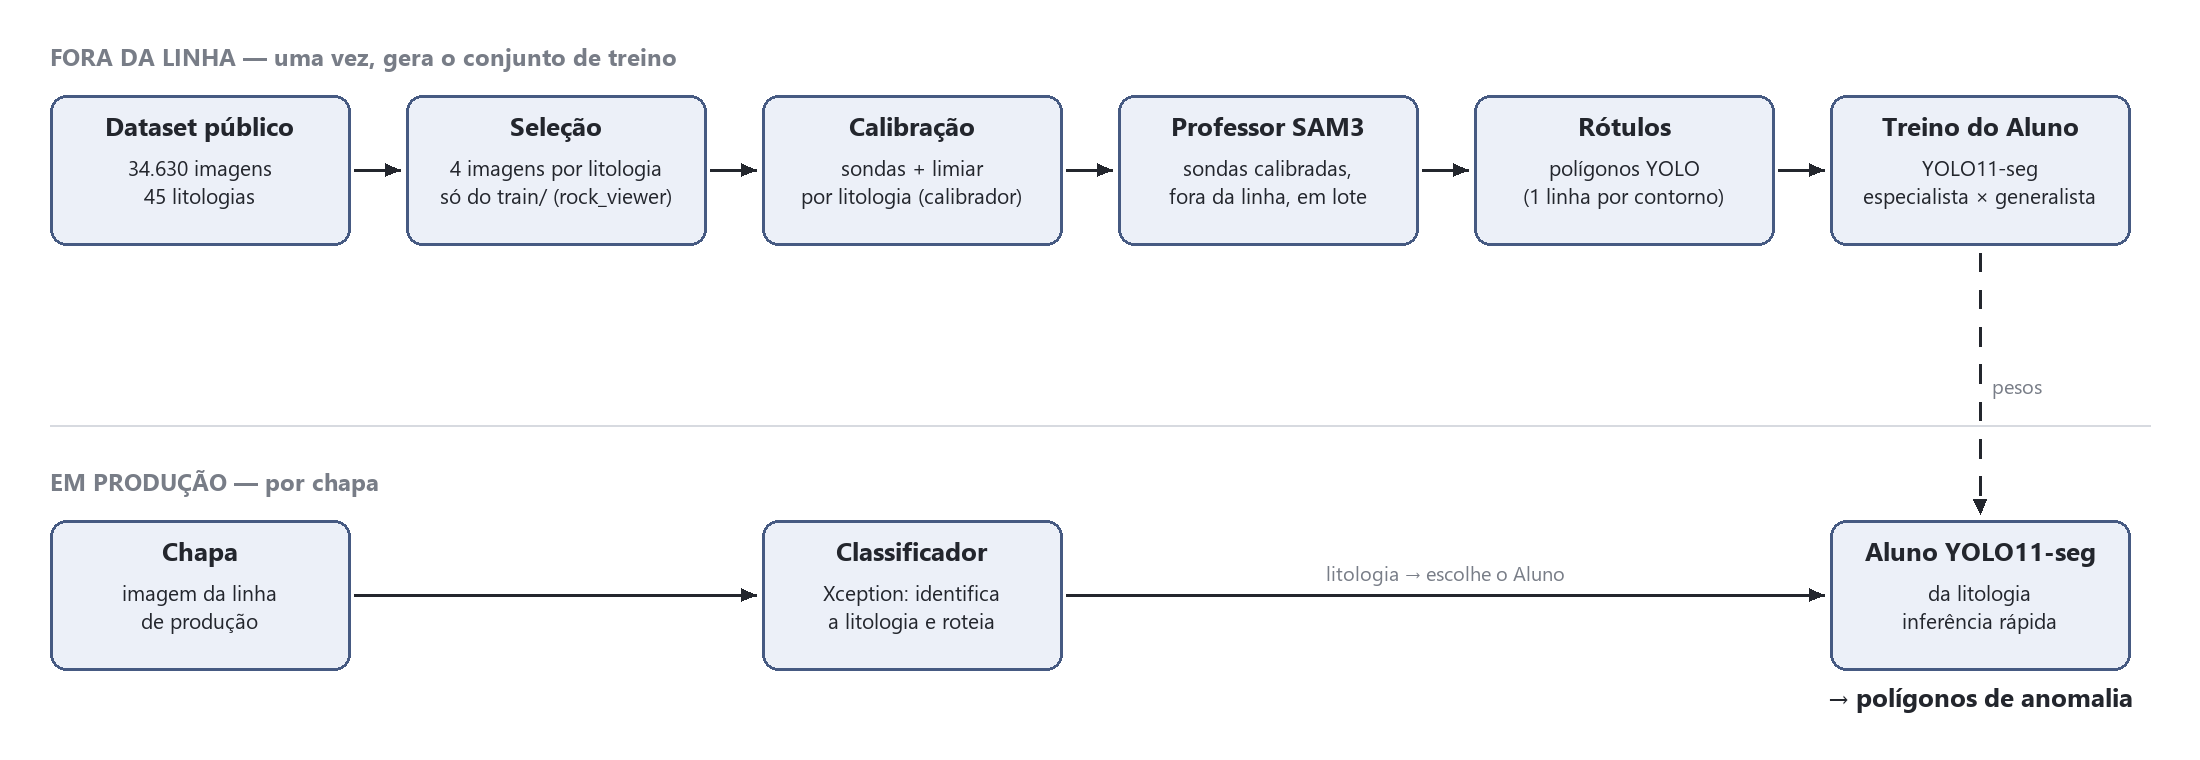
\includegraphics[width=\textwidth]{arquitetura_aria.png}
  \legend{Fonte: elaborado pelo autor.}
\end{figure}

\section{Estágio 1 --- Reprodução do Classificador de Litologias}
\label{sec:classificador}

O classificador do primeiro estágio é uma \textbf{reprodução} do modelo Xception do DeepStoneAI \cite{deepstoneai_moreira2025}, e não o modelo original: o material publicado daquele trabalho traz a receita de treinamento, em cadernos Keras, mas não os pesos treinados. A receita foi mantida --- pesos iniciais do ImageNet, 15 épocas com a base congelada e taxa de aprendizado de $10^{-4}$, ajuste fino das últimas 50 camadas com taxa de $10^{-5}$, aumento de dados por espelhamento, rotação, \textit{zoom} e contraste, e ausência de pesos por classe. Quatro aspectos foram alterados, conforme o Quadro \ref{quad:xception}.

\begin{quadro}[ht]
  \caption{Diferenças entre o classificador original e a reprodução adotada.}
  \label{quad:xception}
  \centering
  \begin{tabularx}{\textwidth}{lXX}
    \hline
    \bfseries Aspecto & \bfseries DeepStoneAI & \bfseries ARIA \\
    \hline
    Arcabouço     & Keras/TensorFlow & PyTorch, com a mesma arquitetura e os mesmos pesos iniciais \\
    Particionamento & Partições originais fundidas e sorteadas de novo por imagem & Partições originais do conjunto de dados, as mesmas da calibração \\
    Resolução     & Carregada em 480 e ampliada para 1.080 \textit{pixels} & 480 $\times$ 480 \textit{pixels}, sem ampliação \\
    Normalização  & Entrada em $[0, 1]$ & Entrada em $[-1, 1]$, a escala esperada pelos pesos do ImageNet \\
    \hline
  \end{tabularx}
  \legend{Fonte: elaborado pelo autor.}
\end{quadro}

A troca de arcabouço é de ordem prática. A alteração do particionamento é metodológica: com as partições originais, o classificador nunca é treinado sobre as imagens de teste das quais saem as chapas da avaliação (Seção \ref{sec:referencia}). A correção da normalização ajusta a entrada à escala para a qual os pesos pré-treinados foram produzidos. A fidelidade da reprodução foi conferida no código, inclusive pela contagem de parâmetros treináveis na fase de ajuste fino, idêntica à do modelo original.

O classificador é avaliado uma única vez sobre a partição de teste, ao final do treinamento, por acurácia, acurácia balanceada e F1 macro.

\section{Sondas de Recall, não Rótulos Semânticos}
\label{sec:sondas}

O Professor é guiado por um conjunto de palavras em inglês, aqui denominadas \textbf{sondas}. O Quadro \ref{quad:sondas} lista o conjunto de trabalho e a assinatura visual que cada sonda costuma ativar.

\begin{quadro}[ht]
  \caption{Sondas textuais, identificadores e assinatura visual associada.}
  \label{quad:sondas}
  \centering
  \begin{tabularx}{\textwidth}{llX}
    \hline
    \bfseries Sonda & \bfseries \textit{id} & \bfseries Assinatura visual que costuma ativar \\
    \hline
    \textit{vein}         & 0 & Estrias e faixas contrastantes \\
    \textit{crack}        & 1 & Descontinuidades lineares finas e escuras \\
    \textit{Stain}        & 2 & Variação de cor em mancha difusa \\
    \textit{Dark patches} & 3 & Regiões escuras sobre fundo claro \\
    \textit{light spot}   & 4 & Regiões claras sobre fundo escuro \\
    \textit{scratch}      & 5 & Riscos superficiais finos \\
    \textit{white stain}  & 6 & Manchas brancas não marcadas por \textit{light spot} \\
    \hline
  \end{tabularx}
  \legend{Fonte: elaborado pelo autor.}
\end{quadro}

É necessário ser explícito quanto ao estatuto dessas palavras. Elas \textbf{não são afirmações sobre a natureza do que foi encontrado}: são chaves lexicais escolhidas por fazerem o modelo responder a certas assinaturas visuais. Afirmar que a região marcada pela sonda \textit{crack} \textit{é} uma fissura exigiria ter validado que o modelo distingue fissura de veio --- validação que este trabalho não realiza e, portanto, não pode alegar.

Dessa decisão decorre a \textbf{rotulagem binária}: todas as regiões marcadas recebem o mesmo identificador de classe no treinamento do Aluno. Os identificadores por sonda listados no Quadro \ref{quad:sondas} são preservados nos arquivos de anotação, para não perder o registro de qual sonda disparou cada região, mas são colapsados em uma única classe antes do treino. O objetivo do conjunto de sondas é maximizar a \textbf{cobertura} de regiões anômalas, não classificá-las. A rotulagem multiclasse fica registrada como trabalho futuro.

O conjunto de sondas não é fechado: ele pode crescer durante a calibração, sob uma condição. Qualquer palavra pode ser testada na ferramenta de calibração como sonda exploratória, com as máscaras exibidas, mas uma sonda só passa a gerar anotação depois de \textbf{registrada}, com identificador próprio --- e só é registrada quando marca regiões que nenhuma das sondas existentes marca. A sonda \textit{white stain} entrou dessa forma: testada sobre a litologia \textit{san\_francisco\_green}, marcou manchas brancas que \textit{light spot} não alcançava. O identificador de uma sonda é permanente, e sondas novas recebem o próximo número livre. Renumerar uma sonda já usada faria os arquivos de anotação gravados antes passarem a indicar outra sonda, sem erro algum que denunciasse a troca. Como os identificadores são colapsados em uma única classe antes do treino, registrar uma sonda a mais amplia a cobertura sem alterar a natureza do rótulo. Nas litologias calibradas antes do registro de uma sonda, ela permanece candidata não avaliada até que a litologia seja revista.

\section{Protocolo de Calibração}
\label{sec:protocolo}

O Professor não é empregado como modelo pronto. O modelo de fundação responde a uma sonda textual sem treinamento no domínio, mas o que ele marca com cada sonda, e a partir de que escore a marcação deixa de ser ruído, varia de uma litologia para outra. A calibração é, portanto, a \textbf{adaptação do Professor ao domínio}, feita sem alterar os pesos do modelo: por litologia, escolhem-se as sondas e o limiar a partir de quatro imagens selecionadas manualmente. A capacidade \textit{zero-shot} é do modelo de fundação; a contribuição do ARIA está em tornar explícita, e registrada, a adaptação que o domínio exige.

Calibrar uma litologia significa responder a duas perguntas distintas: \textit{quais} sondas entram no conjunto, e com \textit{qual} limiar de confiança cada uma opera. A imagem ideal para responder a cada uma é oposta, e confundi-las é a origem de um viés concreto.

Para \textbf{descobrir} quais sondas respondem, a imagem deve conter o máximo de fenômenos --- quanto mais rica, melhor. Para \textbf{escolher} o limiar, a imagem deve representar a variação típica da litologia. Usar a chapa mais rica para as duas tarefas produz um efeito de seleção por visibilidade: as feições foram escolhidas justamente por serem visíveis, e o limiar resultante sai alto demais, perdendo o defeito sutil das demais chapas. Usar a chapa mais sutil produz o erro oposto --- limiar baixo e enxurrada de marcações na chapa comum.

O protocolo adotado separa as duas tarefas em quatro imagens por litologia, descritas no Quadro \ref{quad:vagas}.

\begin{quadro}[ht]
  \caption{As quatro imagens de calibração por litologia e o papel de cada uma.}
  \label{quad:vagas}
  \centering
  \begin{tabularx}{\textwidth}{llX}
    \hline
    \bfseries Imagem & \bfseries Decide & \bfseries Critério de seleção \\
    \hline
    \textit{descoberta}    & Quais sondas entram & A chapa com o maior número de tipos distintos de feição \\
    \textit{limiar sutil}  & O limiar & Feições fracas, de baixo contraste \\
    \textit{limiar típica} & O limiar & A chapa mais comum da litologia \\
    \textit{limiar forte}  & O limiar & Feições marcantes, de alto contraste \\
    \hline
  \end{tabularx}
  \legend{Fonte: elaborado pelo autor.}
\end{quadro}

Três observações completam o protocolo.

Primeiro, as três imagens de limiar \textbf{não produzem três limiares a serem promediados}. Trata-se de um único limiar submetido a três casos. A média de três ótimos não é um ótimo: o caso sutil pediria um valor baixo, o caso forte um valor alto, e a média seria um número nunca verificado em imagem alguma, possivelmente ruim nas duas pontas. A pergunta deixa de ser "qual limiar acerta esta imagem", que não tem resposta, e passa a ser "qual limiar menos erra nas três", que tem.

Segundo, a seleção das quatro imagens é \textbf{manual}. Usar o próprio Professor para escolher as imagens de calibração seria raciocínio circular.

Terceiro, as quatro imagens saem exclusivamente da partição de \textbf{treinamento}. As chapas da avaliação saem da partição de teste, e calibrar sobre uma imagem de teste equivaleria a ajustar o limiar sobre a própria prova. Como as partições não são sorteadas por imagem, um bloco que caiu inteiro na partição de teste não é visto durante a calibração, o que torna a avaliação mais exigente: ela mede a marcação inclusive em chapas que a calibração não teve como antecipar. Para as litologias da faixa A, a partição de treinamento reúne de 700 a 3.200 imagens, e o que limita a cobertura na escolha das imagens de calibração é a varredura do autor, não o tamanho da partição.

A origem de cada imagem selecionada --- partição e arquivo --- é registrada em um arquivo de metadados por litologia, compondo o material de reprodutibilidade do trabalho.

\subsection{Litologias movimentadas}
\label{sec:movimentadas}

Durante a seleção das imagens da faixa A, o autor encontrou litologias de padrão movimentado, em que é difícil distinguir o que é defeito do que é o próprio desenho da pedra: o padrão natural já contém manchas, veios e contrastes fortes, e uma mesma feição pode valorizar a chapa ou desqualificá-la. Quatro litologias da faixa A foram identificadas assim pelo autor: \textit{shadow\_white}, \textit{san\_francisco\_green}, \textit{white\_mirage} e \textit{golden\_storm}.

Essas litologias são calibradas pelo mesmo protocolo das demais. Excluí-las retiraria quatro das onze litologias da faixa A e exigiria um critério de exclusão que não existe por escrito --- o que reproduziria, na seleção do experimento, o problema que o trabalho aponta na inspeção. A dificuldade de julgá-las também não é um desvio do trabalho: é a arbitrariedade da fronteira entre feição e defeito no seu caso mais forte, e por isso elas são o melhor teste do protocolo. O que se observou nelas está na Seção \ref{sec:res_calibracao}.

O termo adotado é \textbf{movimentada}, em oposição a homogênea. A classificação, que \citeonline[p.~920]{camargo_geociencias2015} atribuem a Meyer (2003), separa os materiais pelo padrão textural e estrutural: os homogêneos têm estrutura isotrópica, sem orientação mineral definida; os movimentados apresentam estrutura ou textura definida pela concentração ou pela orientação preferencial de seus minerais, como bandamento ou foliação. O termo ``exótica'', que circula no setor, foi evitado por designar uma categoria comercial, ligada a raridade e preço, que não descreve a dificuldade observada.

\section{A Regra que Produz o Limiar}
\label{sec:regra}

A escolha do limiar precisa ser governada por uma regra escrita. Selecionar o valor "no olho", ainda que por um observador experiente, reproduziria exatamente a prática que o Capítulo 1 aponta como problema --- com a diferença de que o observador passaria a ser o autor, em vez do inspetor.

Estabelece-se, portanto, a seguinte distinção, que é o núcleo do desenho:

\begin{description}
  \item[O valor do limiar] \textbf{muda} por litologia. É o objetivo da calibração.
  \item[A regra que produz o valor] \textbf{não muda}. É idêntica para todas as 45 litologias.
\end{description}

A regra adotada é a seguinte. Para cada sonda, constrói-se a curva que relaciona o limiar ao número de regiões marcadas, somando as três imagens de limiar da litologia. O limiar escolhido é o \textbf{joelho} dessa curva, definido como o ponto de máxima distância à corda que liga seus dois extremos, após normalização dos eixos \cite{kneedle_satopaa2011}.

Formalmente, seja $V = \{\text{sutil}, \text{típica}, \text{forte}\}$ o conjunto das imagens de limiar de uma litologia e $D_v$ o conjunto das detecções de uma sonda na imagem $v$, obtidas com o limiar no piso, cada detecção $d$ com escore $s_d$. A curva da regra é dada pela Equação \ref{eq:curva}:

\begin{equation}
  N(t) = \sum_{v \in V} \left| \{\, d \in D_v : s_d > t \,\} \right|
  \label{eq:curva}
\end{equation}

\noindent avaliada em uma grade de 80 limiares $t_1 < t_2 < \dots < t_n$ em progressão geométrica, entre 0,9 vez o menor e o maior escore observado nas três imagens. Os dois eixos são normalizados no intervalo $[0, 1]$, o do limiar em escala logarítmica:

\begin{equation}
  x_i = \frac{\ln t_i - \ln t_1}{\ln t_n - \ln t_1}, \qquad
  y_i = \frac{N(t_i) - \min_j N(t_j)}{\max_j N(t_j) - \min_j N(t_j)}
  \label{eq:normalizacao}
\end{equation}

\noindent Como $N$ é decrescente, os extremos normalizados são $(0, 1)$ e $(1, 0)$, e a corda que os liga é a reta $x + y - 1 = 0$. O limiar da regra é o ponto da grade mais distante dessa corda (Equação \ref{eq:joelho}):

\begin{equation}
  t^{*} = t_{i^{*}}, \qquad
  i^{*} = \arg\max_{i} \frac{\left| x_i + y_i - 1 \right|}{\sqrt{2}}
  \label{eq:joelho}
\end{equation}

A forma da regra foi escolhida entre duas alternativas. A outra fixaria o limiar como o maior valor que ainda marca uma fração mínima das feições anotadas nas imagens de limiar. Seria uma regra mais próxima do objetivo final, por medir acerto em vez de forma de curva, mas exigiria anotar manualmente as três imagens de limiar de cada litologia --- 135 imagens com polígonos desenhados à mão --- e ainda introduziria um parâmetro livre, a fração mínima. O joelho dispensa anotação e não tem parâmetro a fixar. Sua adequação é verificada sem custo adicional, pela mesma auditoria cega que avalia o Experimento 1 (Seção \ref{sec:referencia}).

Três aspectos da regra são fixados deliberadamente. A imagem de \textit{descoberta} \textbf{não} entra no cálculo: escolhida por ser a mais rica em feições, ela puxaria o limiar para cima, reintroduzindo o viés de seleção por visibilidade que o protocolo existe para evitar. O eixo do limiar é tomado em escala \textbf{logarítmica}, porque os escores concentram-se na década baixa --- medidos entre 0,011 e 0,770 em uma litologia de referência, com mediana entre 0,040 e 0,080 --- e, em escala linear, o joelho recairia sistematicamente sobre o primeiro ponto da curva. Por fim, a regra \textbf{não possui parâmetro livre}: não há constante a ser fixada por inspeção, o que elimina a possibilidade de ajustá-la para favorecer um resultado.

A regra é aplicada mecanicamente. Reconhece-se, porém, que uma curva pode enganar em casos particulares, e o autor pode divergir do valor produzido. Para que essa divergência não se torne invisível, a ferramenta de calibração registra \textbf{ambos} os valores --- o produzido pela regra e o adotado pelo autor --- junto de uma justificativa textual obrigatória. Na litologia \textit{siena\_white}, por exemplo, o critério registrado foi: ``Subi até o ponto em que a vaga típica para de marcar matriz limpa, aceitando perder feições mais fracas da vaga sutil; a vaga forte continua com todas as óbvias.'' A justificativa nomeia o que foi aceito perder, e é isso que a torna auditável: outra pessoa pode discordar do limiar sabendo exatamente que troca foi feita. Os dois valores têm papéis distintos no Experimento 1: o da regra alimenta os braços que testam a regra, e o adotado pelo autor ocupa um braço próprio, que mede o efeito do ajuste humano (Seção \ref{sec:exp1}). O valor adotado pelo autor é também o que rotula o conjunto de treinamento do Aluno, e deixá-lo fora do experimento significaria avaliar uma configuração que o sistema não usa. A taxa de concordância entre regra e autor é reportada como resultado à parte, e constitui evidência sobre a adequação da própria regra.

\section{Varredura de Limiares Fora de Linha}
\label{sec:varredura}

Calibrar exige comparar muitos limiares. Feito de modo ingênuo --- escolher um valor, executar o Professor, observar, ajustar e reexecutar --- cada iteração custa minutos de processamento em GPU, o que inviabiliza o protocolo da seção anterior em tempo humano.

A inspeção do código do arcabouço utilizado mostra que o limiar de confiança é aplicado como \textbf{filtro posterior} à inferência. O modelo produz máscaras e escores sem conhecimento do limiar; este apenas descarta as detecções cujo escore não o ultrapassa. A supressão de não-máximos ocorre depois do filtro, mas processa as detecções em ordem decrescente de escore e só remove uma detecção usando outra de escore \textbf{maior} --- de onde se conclui que incluir detecções de escore baixo não altera as decisões tomadas sobre as de escore alto.

Segue-se que executar o Professor uma única vez com o limiar no piso, armazenar escores e polígonos, e filtrar esse material posteriormente é \textbf{exatamente equivalente} a reexecutar o modelo em cada limiar --- não se trata de aproximação. O ciclo de calibração passa de minutos por iteração a milissegundos, e é o que torna viável exibir simultaneamente o efeito de um mesmo limiar sobre as quatro imagens da litologia.

A equivalência não foi assumida: ela é verificada experimentalmente, e o procedimento de verificação é descrito na Seção \ref{sec:verificacao} e seu resultado reportado no Capítulo 4.

\section{Ferramentas de Seleção e Calibração}
\label{sec:ferramentas}

O protocolo das seções anteriores é executado com duas ferramentas desenvolvidas para este trabalho e mantidas no repositório. As responsabilidades são separadas de propósito: a ferramenta de seleção apenas escolhe as quatro imagens de cada litologia; a de calibração apenas decide quais sondas entram e com que limiar; e somente o \textit{script} de inferência do Professor grava as anotações finais. Nenhuma das duas primeiras produz rótulo de treinamento.

\subsection{Seleção das imagens}

A ferramenta de seleção exibe, no navegador, a grade de todas as imagens da partição de treinamento de uma litologia, conforme a Figura \ref{fig:rock_viewer}. O cabeçalho mostra a faixa de volume, o total de imagens, as quatro vagas com seu estado e a instrução da vaga em preenchimento --- para a vaga de descoberta, por exemplo, a de procurar a chapa com o maior número de tipos distintos de feição. Cada imagem pode ser ampliada e percorrida pelo teclado, e a escolha é confirmada digitando-se seu número.

\begin{figure}[ht]
  \caption{Ferramenta de seleção: grade de imagens de uma litologia, com as quatro vagas e a instrução da vaga em preenchimento.}
  \label{fig:rock_viewer}
  \centering
  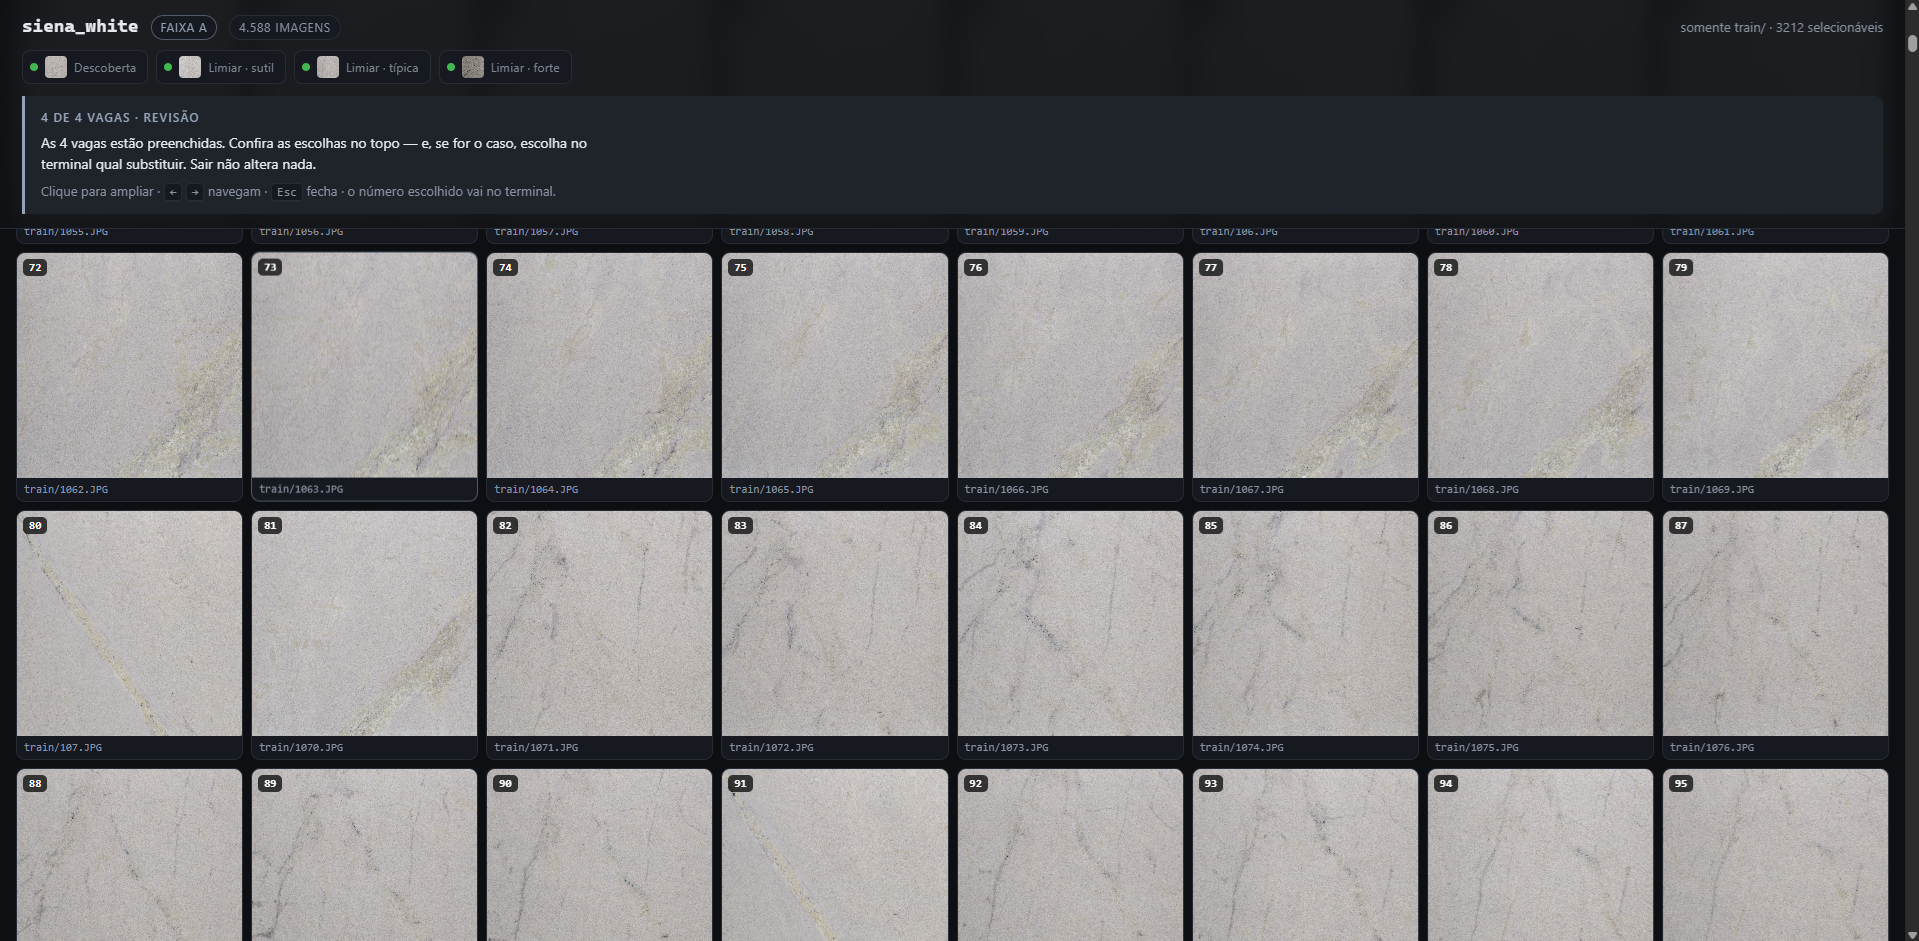
\includegraphics[width=\textwidth]{rock_viewer.png}
  \legend{Fonte: elaborado pelo autor.}
\end{figure}

Três propriedades do protocolo são garantidas pela ferramenta, e não pela disciplina de quem a opera. Somente imagens da partição de treinamento podem ser escolhidas; as das demais partições podem ser exibidas para estudo da variabilidade da rocha, mas aparecem bloqueadas e são recusadas. As litologias são oferecidas em ordem de volume de dados, da faixa A para a D, de modo que a ordem de trabalho é a própria prioridade do experimento. E cada escolha é copiada para um arquivo nomeado pelo papel da vaga, com a partição, o arquivo de origem e a data registrados nos metadados da litologia.

\subsection{Calibração}

A ferramenta de calibração é uma aplicação web local organizada em três etapas, que correspondem às duas perguntas da Seção \ref{sec:regra} e ao registro da resposta. A única etapa que usa a GPU é a captura: o Professor é executado com o limiar no piso sobre cada par (imagem, sonda) ainda sem material armazenado. Tudo o que vem depois opera sobre esse material, pela equivalência da Seção \ref{sec:varredura}.

Na etapa de \textbf{descoberta} (Figura \ref{fig:calib_descoberta}), cada sonda candidata é exibida sobre a imagem de descoberta, com o número de detecções e a faixa de escores. O limiar usado nessa tela serve apenas para visualizar e não é gravado: a pergunta é se a sonda responde a algo que existe na rocha, e não onde cortá-la. O autor marca as sondas que entram no conjunto; sondas exploratórias ainda não registradas podem ser vistas, mas não marcadas.

\begin{figure}[ht]
  \caption{Calibração, etapa de descoberta: as sondas candidatas sobre a imagem de descoberta.}
  \label{fig:calib_descoberta}
  \centering
  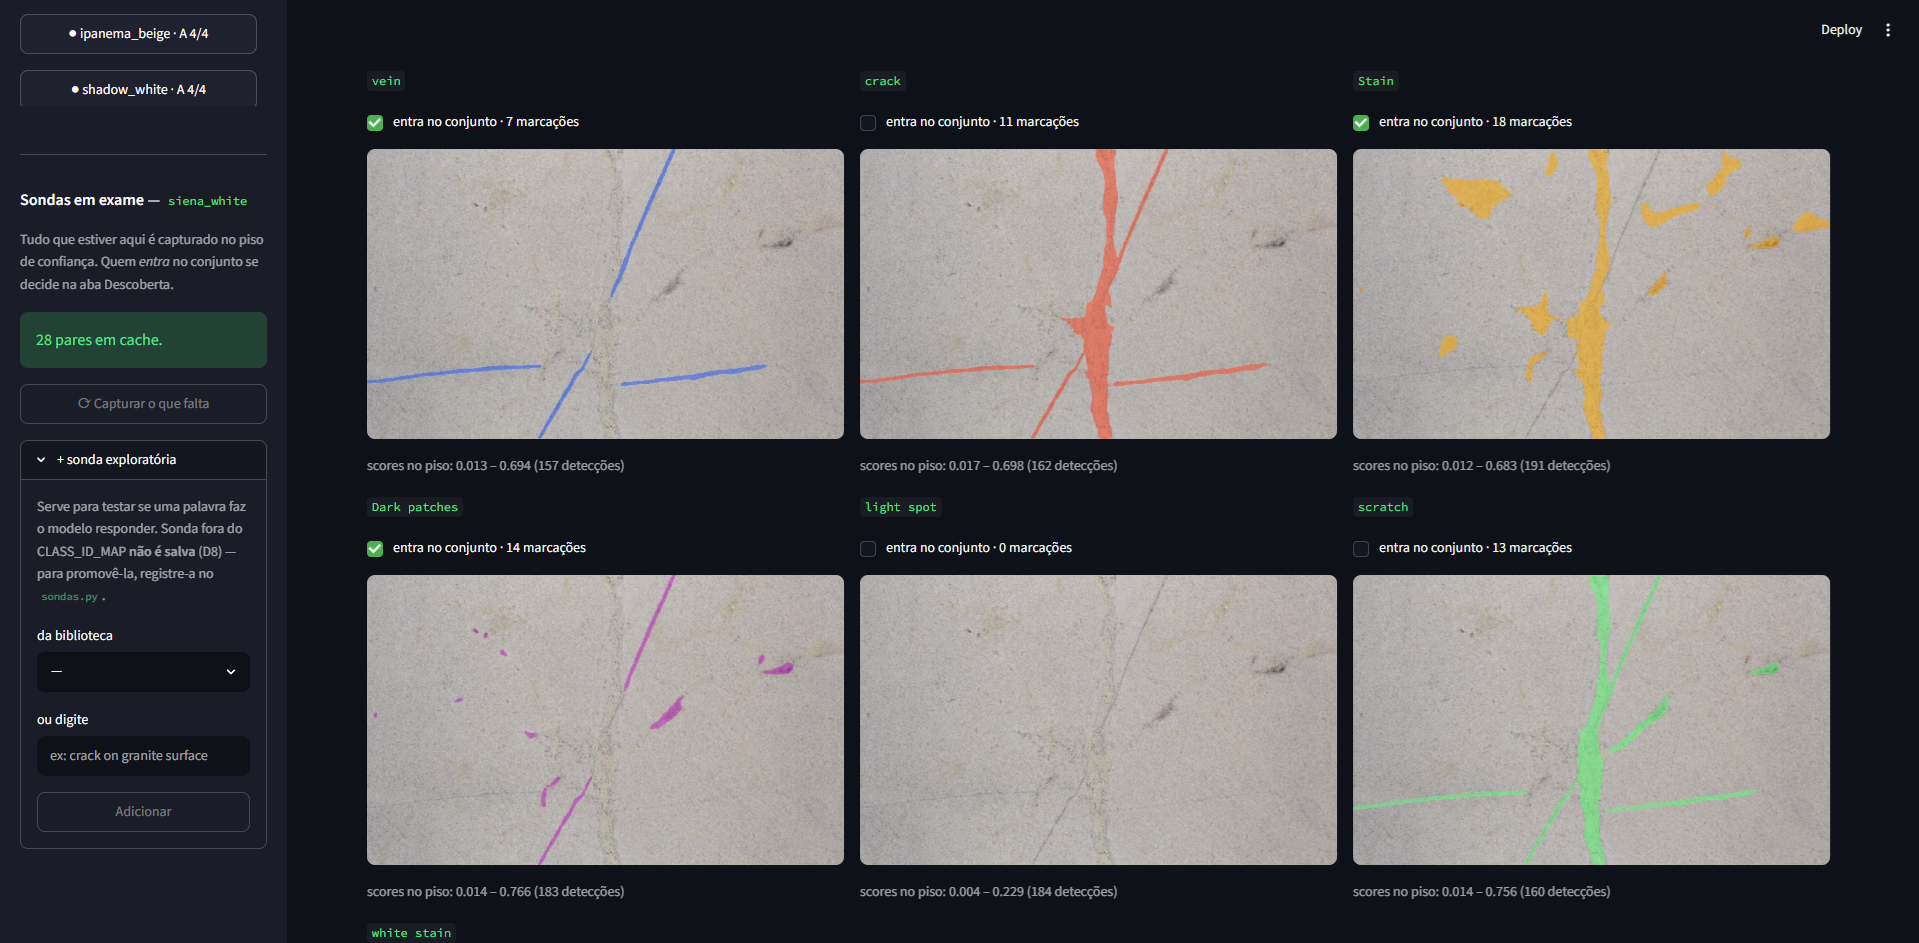
\includegraphics[width=\textwidth]{calib_descoberta.png}
  \legend{Fonte: elaborado pelo autor.}
\end{figure}

Na etapa de \textbf{limiar} (Figura \ref{fig:calib_limiar}), um único controle de limiar por sonda governa quatro prévias simultâneas, uma por imagem, cada uma com sua contagem de marcações. É a forma visual do princípio da Seção \ref{sec:regra}: um limiar submetido a três casos, e não três limiares a serem combinados. Abaixo das prévias, a curva da Equação \ref{eq:curva} é traçada por imagem, em escala logarítmica, com o limiar corrente e o limiar da regra marcados. O controle parte do valor da regra; o autor diverge dele se quiser, e nunca o contrário.

\begin{figure}[ht]
  \caption{Calibração, etapa de limiar: um controle, quatro prévias simultâneas e a curva com o limiar da regra marcado.}
  \label{fig:calib_limiar}
  \centering
  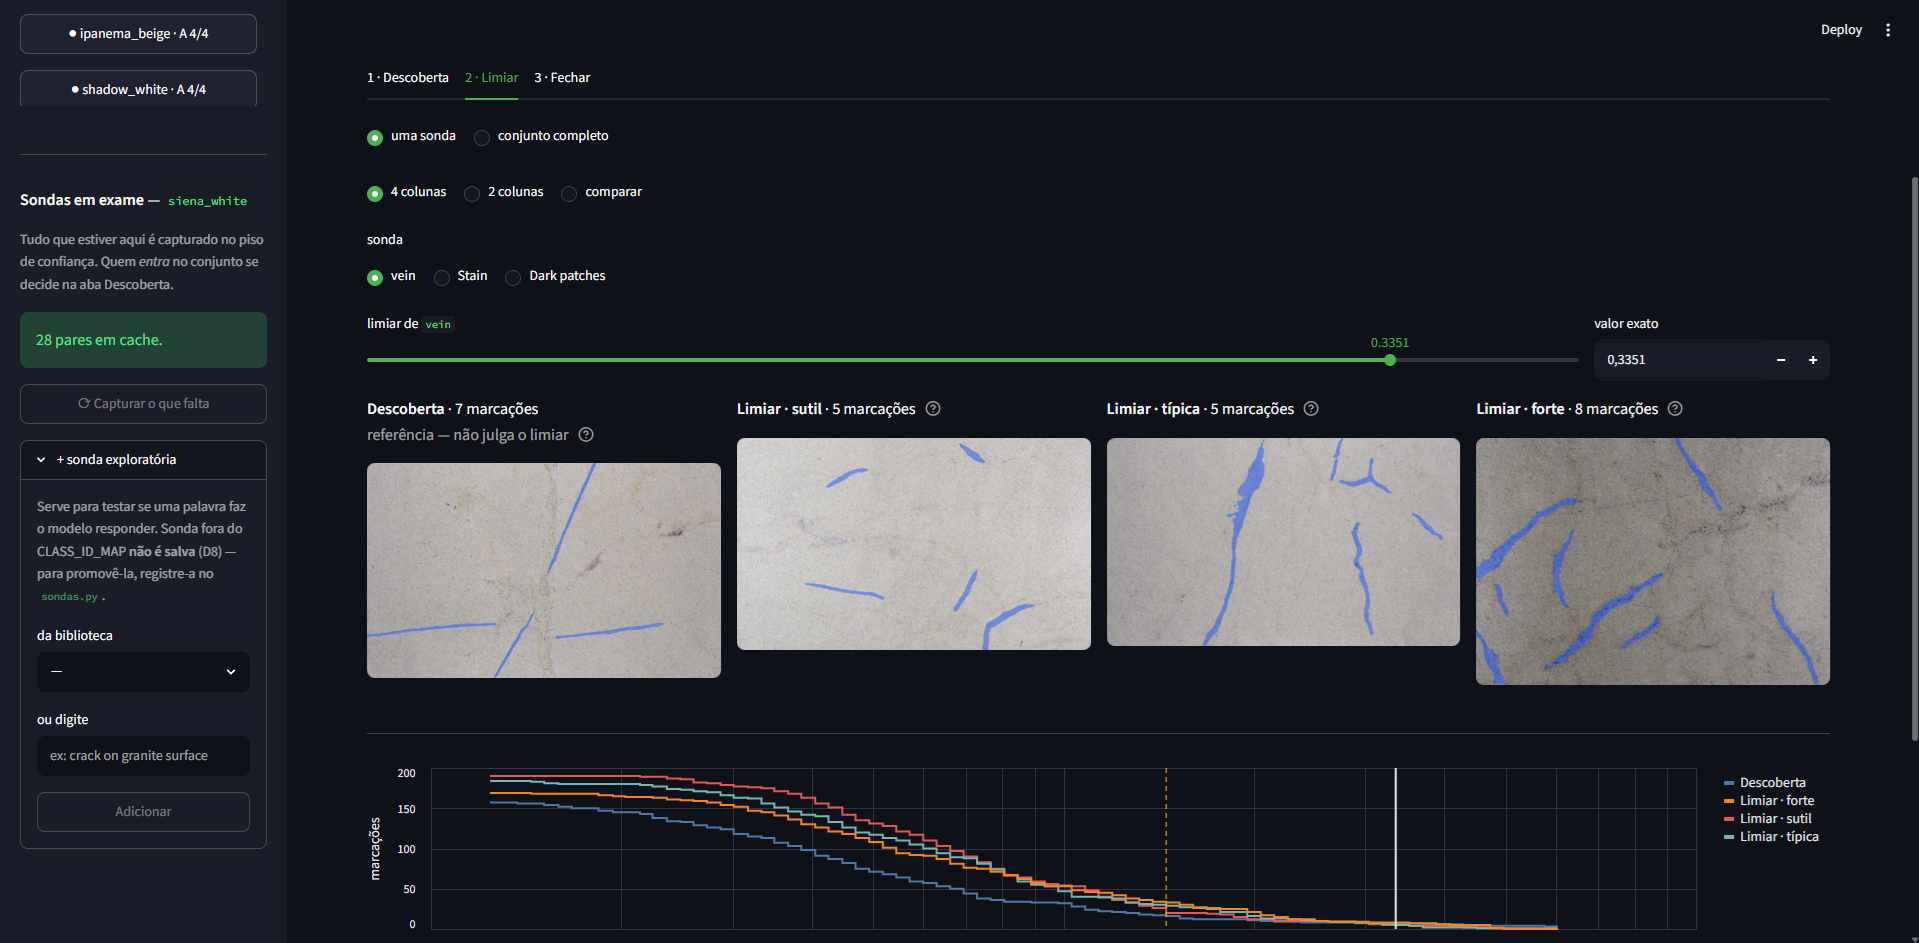
\includegraphics[width=\textwidth]{calib_limiar.png}
  \legend{Fonte: elaborado pelo autor.}
\end{figure}

Na etapa de \textbf{fechamento} (Figura \ref{fig:calib_fechar}), uma tabela reúne, por sonda, o limiar da regra, o adotado pelo autor, a divergência entre os dois e as marcações em cada imagem. O salvamento permanece bloqueado enquanto o campo do critério estiver vazio: não é possível gravar um limiar sem escrever por que ele foi escolhido.

\begin{figure}[ht]
  \caption{Calibração, etapa de fechamento: regra, limiar do autor e divergência por sonda, e o campo obrigatório do critério.}
  \label{fig:calib_fechar}
  \centering
  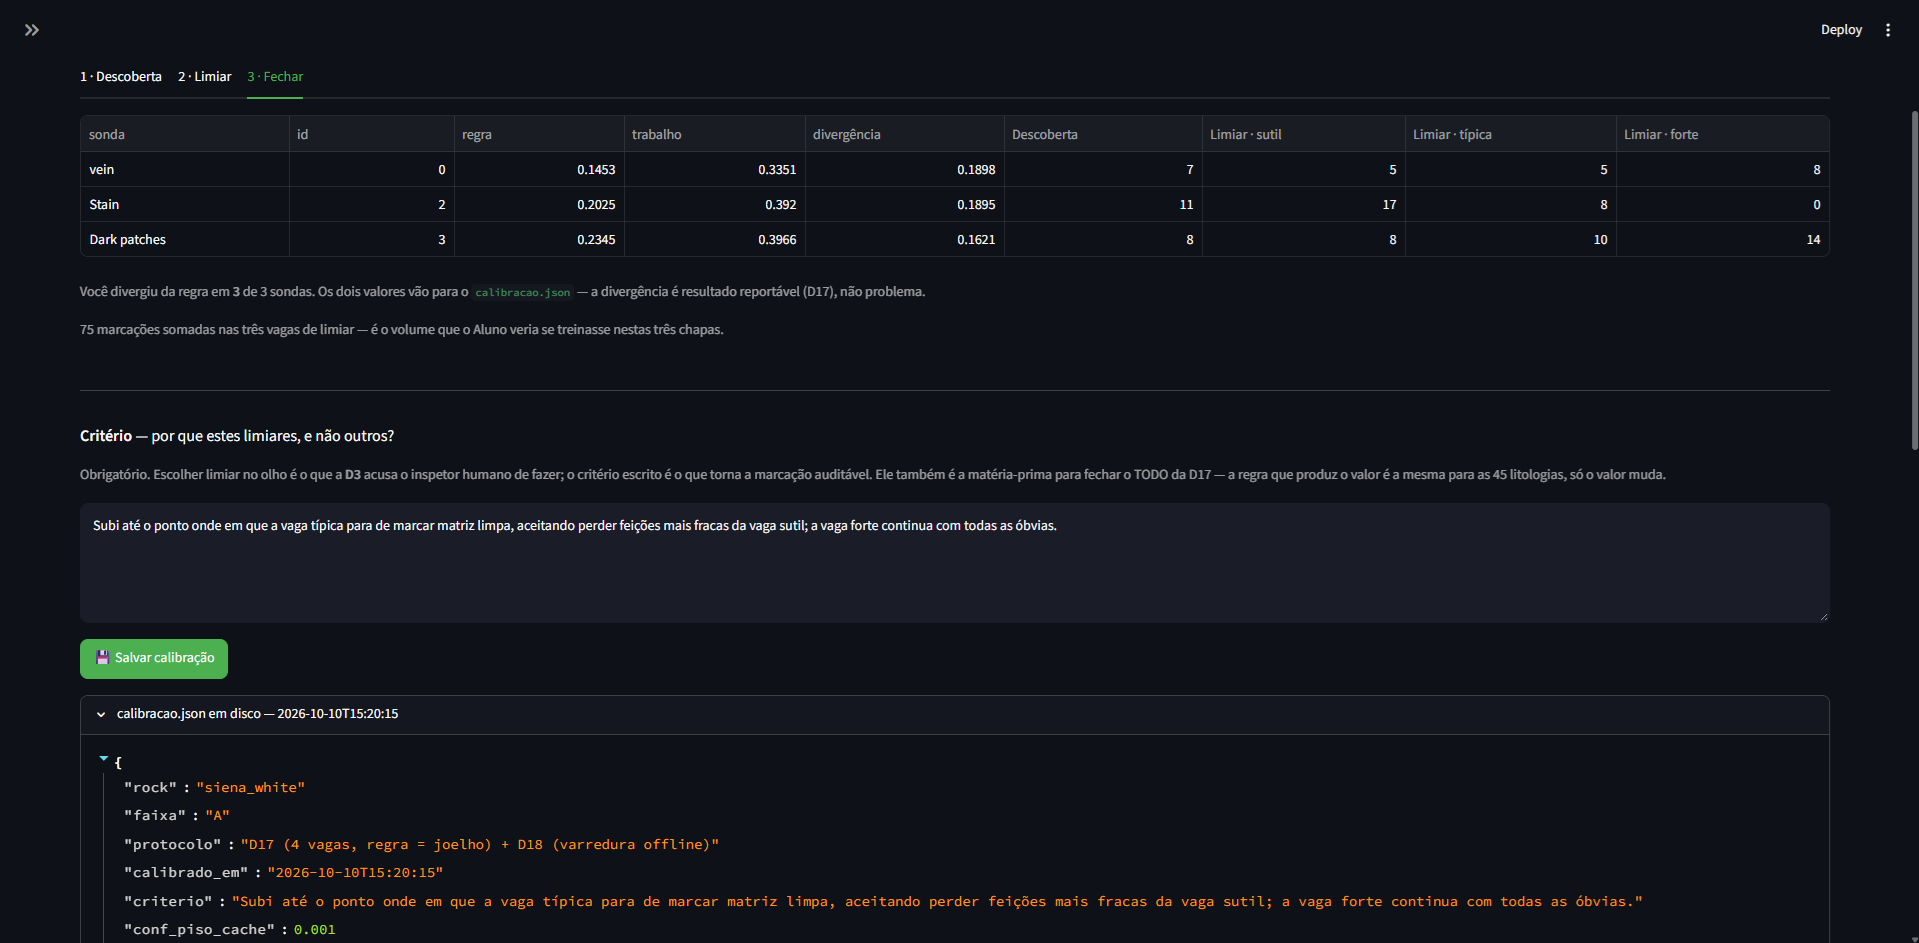
\includegraphics[width=\textwidth]{calib_fechar.png}
  \legend{Fonte: elaborado pelo autor.}
\end{figure}

\subsection{O registro de calibração}

O salvamento produz o registro de calibração da litologia, um arquivo de texto versionado junto do código. O Código \ref{lst:calibracao} mostra um trecho do registro da \textit{siena\_white}, com uma das três sondas do conjunto.

\begin{lstlisting}[caption={Trecho do registro de calibração da litologia \textit{siena\_white}.}, label={lst:calibracao}, literate={á}{{\'a}}1 {é}{{\'e}}1 {í}{{\'i}}1 {ó}{{\'o}}1 {ú}{{\'u}}1 {ã}{{\~a}}1 {õ}{{\~o}}1 {ç}{{\c{c}}}1 {â}{{\^a}}1 {ê}{{\^e}}1 {ô}{{\^o}}1]
{
  "rock": "siena_white",
  "faixa": "A",
  "protocolo": "D17 (4 vagas, regra = joelho) + D18 (varredura offline)",
  "calibrado_em": "2026-10-10T15:20:15",
  "criterio": "Subi até o ponto [...]",
  "conf_piso_cache": 0.001,
  "ultralytics": "8.4.61",
  "sondas_na_regra": 0,
  "sondas_divergentes": ["vein", "Stain", "Dark patches"],
  "sondas": {
    "vein": {
      "limiar_trabalho": 0.3351,
      "limiar_regra": 0.1453,
      "divergencia": 0.1898,
      "marcacoes_por_vaga": {
        "descoberta": 7, "limiar_sutil": 5,
        "limiar_tipica": 5, "limiar_forte": 8
      }
    }
  }
}
\end{lstlisting}

Cada campo responde a uma pergunta que um auditor faria. O critério diz por que o limiar é aquele. Os dois limiares e a divergência dizem quanto do valor veio da regra e quanto do autor. As contagens por imagem permitem conferir o efeito do limiar sem reexecutar nada. O piso e a versão da biblioteca dizem sob que condições a varredura fora de linha foi exata. É esse arquivo, e não o modelo treinado, que materializa a contribuição do trabalho: o critério de marcação de uma litologia, escrito em um lugar onde pode ser lido, contestado e versionado.

\section{Avaliação por Auditoria Cega}
\label{sec:referencia}

Toda métrica de acerto exige uma referência externa ao modelo. Usar a saída do próprio Professor como referência mediria fidelidade de cópia, e não acerto, e tornaria sem sentido a comparação entre configurações --- cada uma teria um gabarito diferente. A referência adotada é o \textbf{julgamento humano}, obtido por auditoria cega das marcações.

\subsection{Procedimento}

A amostra de avaliação reúne três chapas por litologia da faixa A, sorteadas com semente fixa da partição de \textbf{teste}: 33 chapas que nenhuma etapa da calibração viu. O Professor é executado uma única vez sobre cada uma, com todas as sondas e o limiar no piso, e os quatro braços do Experimento 1 (Seção \ref{sec:exp1}) são aplicados como filtros desse material. O \textbf{conjunto reunido} é formado por toda detecção que ao menos um braço marcaria.

As detecções são apresentadas ao avaliador uma a uma, em um aplicativo desenvolvido para este fim, que exibe a região contornada, ampliada, ao lado da chapa inteira, e faz sempre a mesma pergunta: \textit{numa inspeção de qualidade, você marcaria esta região como defeito?} As respostas possíveis são sim, não e não sei. O aplicativo não informa de que braço, de que sonda ou de que litologia vem cada marcação, nem o seu escore. Como os braços são filtros do mesmo material, uma detecção pertence em geral a vários deles, e o julgamento de cada detecção vale para todos os braços que a contêm --- de modo que a auditoria é cega quanto ao braço por construção.

O conjunto reunido é grande demais para ser julgado por inteiro, e por isso é amostrado. As detecções são agrupadas em \textbf{estratos}, definidos pelo padrão de pertencimento aos quatro braços, e cada estrato contribui com o mesmo número de itens, o que garante julgamentos suficientes também para os braços que marcam pouco. Os itens são apresentados em ordem intercalada entre estratos, de modo que qualquer trecho inicial da lista já constitui uma amostra estratificada, e a avaliação pode ser interrompida e retomada sem perda.

\subsection{Métricas}

Seja $h$ um estrato, $N_h$ o número de detecções do conjunto reunido que ele contém e $\hat{p}_h$ a fração julgada como defeito entre os itens julgados do estrato, desconsideradas as respostas ``não sei''. Para um braço $b$, seja $H_b$ o conjunto dos estratos cujas detecções ele marca. A precisão do braço é a fração de suas marcações julgadas como defeito, estimada com peso proporcional ao tamanho de cada estrato (Equação \ref{eq:precisao}):

\begin{equation}
  P_b = \frac{\sum_{h \in H_b} N_h \, \hat{p}_h}{\sum_{h \in H_b} N_h}
  \label{eq:precisao}
\end{equation}

O \textit{recall} absoluto exigiria conhecer todas as anomalias de cada chapa, inclusive as que nenhum braço marcou. Adota-se o \textbf{\textit{recall} relativo} ao conjunto reunido, recurso consolidado na avaliação de sistemas de recuperação de informação, em que se mostra que a ordem relativa entre sistemas avaliados sobre o conjunto reunido de suas respostas é confiável \cite{pooling_zobel1998}. O denominador é o total de acertos dos quatro braços juntos (Equação \ref{eq:recall_rel}):

\begin{equation}
  R_b = \frac{\sum_{h \in H_b} N_h \, \hat{p}_h}{\sum_{h} N_h \, \hat{p}_h}
  \label{eq:recall_rel}
\end{equation}

Uma anomalia que nenhum braço marcou fica fora do denominador de todos eles, de modo que a comparação entre braços permanece justa. Os intervalos de confiança de 95\% são obtidos por reamostragem \textit{bootstrap} dentro de cada estrato \cite{bootstrap_efron1979}, e as diferenças entre braços usam as mesmas reamostragens. Falso positivo, nesta avaliação, é a marcação julgada como não defeito.

\subsection{Avaliadores e concordância}

A avaliação principal é feita por uma estudante de Engenharia de Minas, que não participou da calibração e não conhece a configuração de nenhum braço. O autor julga a mesma amostra, separadamente e sem acesso às respostas dela. A concordância entre os dois é medida pelo coeficiente kappa de Cohen \cite{kappa_cohen1960}, em que $p_o$ é a proporção de itens com a mesma resposta e $p_e$ a proporção esperada ao acaso (Equação \ref{eq:kappa}):

\begin{equation}
  \kappa = \frac{p_o - p_e}{1 - p_e}
  \label{eq:kappa}
\end{equation}

A concordância tem papel próprio no trabalho: ela mede, entre duas pessoas e sobre as mesmas marcações, a arbitrariedade do critério de marcação que o Capítulo 1 descreve.

\section{Experimento 1 --- Critério por Litologia \textit{versus} Critério Único}
\label{sec:exp1}

O primeiro experimento avalia H1 e não envolve treinamento algum: compara configurações do Professor sobre as mesmas imagens, no mesmo modelo e no mesmo equipamento.

O ponto delicado do desenho é a definição do braço de controle. Uma configuração única escolhida arbitrariamente tornaria a comparação vazia, pois o resultado dependeria dessa escolha. O braço de controle é, portanto, \textbf{derivado por regra}, e não selecionado: aplica-se a \textbf{mesma regra} da Seção \ref{sec:regra}, alterando-se o escopo do material sobre o qual ela é calculada. Sonda por sonda, reúnem-se os escores das três imagens de limiar de todas as litologias em um único conjunto, aplica-se a regra e obtém-se um limiar global por sonda.

Comparar esse controle diretamente à configuração calibrada, contudo, alteraria duas coisas ao mesmo tempo. O controle usa todas as sondas cadastradas, enquanto a configuração calibrada usa apenas as que a imagem de descoberta admitiu naquela litologia; um ganho de \textit{recall} do controle não seria atribuível nem ao limiar nem à seleção de sondas. O experimento tem, por isso, quatro braços, cada um diferente do anterior em um único fator, conforme a Tabela \ref{tab:bracos_exp1}.

\begin{table}[ht]
  \caption{Braços do Experimento 1. Cada braço difere do anterior em um único fator.}
  \label{tab:bracos_exp1}
  \centering
  \begin{tabularx}{\textwidth}{lllX}
    \hline
    \bfseries Braço & \bfseries Sondas & \bfseries Limiar & \bfseries Mede, em relação ao anterior \\
    \hline
    Único                  & Todas                    & Regra sobre todas as litologias reunidas & --- \\
    Regra, todas as sondas & Todas                    & Regra sobre a litologia                  & O escopo do limiar: o teste de H1 \\
    Regra, sondas do autor & Admitidas na descoberta  & Regra sobre a litologia                  & A seleção de sondas: o \textit{recall} que ela custa e a precisão que oferece \\
    Calibrado pelo autor   & Admitidas na descoberta  & Adotado pelo autor                       & O ajuste humano do limiar \\
    \hline
  \end{tabularx}
  \legend{Fonte: elaborado pelo autor.}
\end{table}

A comparação entre os dois primeiros braços é o teste de H1. As duas seguintes decompõem o conhecimento de domínio embutido na calibração: quanto do efeito vem de escolher as sondas por litologia e quanto vem do julgamento de quem calibra. A comparação direta entre o braço único e o calibrado pelo autor altera vários fatores de uma vez e pode ser exibida, mas não constitui evidência de H1. Os quatro braços não exigem execução adicional do modelo: pela equivalência demonstrada na Seção \ref{sec:varredura}, o Professor é executado uma única vez com todas as sondas sobre cada chapa da amostra de avaliação, e os braços são filtros distintos do mesmo material.

O braço que isola a seleção de sondas mede o tamanho de uma questão que o desenho não resolve: se uma única imagem de descoberta basta para escolher as sondas de uma litologia. Em litologias cujas feições variam ao longo do bloco, uma chapa distante da escolhida pode apresentar anomalias que nenhuma das sondas admitidas cobre. Se a seleção custar \textit{recall} demais, a alternativa é admitir todas as sondas e calibrar apenas o limiar --- decisão que depende do resultado medido e, por isso, não é antecipada.

Cabe justificar por que o braço único não é definido como a mediana dos limiares calibrados, alternativa aparentemente natural. Se o fosse, o resultado seria quase aritmético: o valor ótimo de cada litologia supera a mediana dos valores ótimos \textbf{nos dados dessa mesma litologia} por construção, o que caracteriza regressão à média e não achado experimental --- além de tornar o controle uma função do tratamento. A regra aplicada ao material reunido é o contrafactual honesto: \textit{e se todas as litologias tivessem sido tratadas como uma só?}, que é precisamente o que H1 pergunta. Esse desenho admite resultado negativo, e é isso que torna a hipótese falseável.

Os quatro braços são avaliados pela auditoria cega da Seção \ref{sec:referencia}, reportando-se precisão e \textit{recall} relativo de cada um, para o conjunto das litologias e para os recortes de litologias movimentadas e demais (Seção \ref{sec:movimentadas}).

\section{Experimento 2 --- Especialistas \textit{versus} Generalista}

O segundo experimento avalia H2 e compara modelos Aluno treinados sobre as anotações do Professor, em três braços, descritos no Quadro \ref{quad:bracos_exp2}.

\begin{quadro}[ht]
  \caption{Braços do Experimento 2.}
  \label{quad:bracos_exp2}
  \centering
  \begin{tabularx}{\textwidth}{lX}
    \hline
    \bfseries Braço & \bfseries Descrição \\
    \hline
    Especialista & Um modelo por litologia, treinado apenas com as anotações daquela litologia \\
    Generalista  & Um único modelo, treinado com as anotações de todas as litologias \\
    Controle     & Um único modelo, treinado com anotações calibradas por litologia \\
    \hline
  \end{tabularx}
  \legend{Fonte: elaborado pelo autor.}
\end{quadro}

O braço de controle existe por necessidade de desenho: sem ele, a comparação entre especialistas e generalista alteraria simultaneamente duas variáveis --- a quantidade de modelos e a especificidade das anotações --- e nenhum resultado seria atribuível a uma delas.

Os resultados são reportados \textbf{por faixa} de volume, e não agregados, o que responde à segunda metade de H2.

Cada modelo especialista é treinado com uma fração dos dados vistos pelo generalista, de modo que a comparação mede o efeito \textbf{líquido} da especialização em cada volume de dados --- e é a estratificação por faixa que torna esse efeito interpretável.

\section{Ambiente Experimental e Reprodutibilidade}
\label{sec:verificacao}

O trabalho foi executado em duas máquinas, com equipamento e versões de bibliotecas diferentes, descritas no Quadro \ref{quad:ambiente}. A diferença não foi uniformizada: o que importa para a validade dos resultados é a versão da biblioteca de modelos, e não a máquina, e por isso cada registro de calibração grava a versão sob a qual foi produzido.

\begin{quadro}[ht]
  \caption{Ambientes de execução dos experimentos.}
  \label{quad:ambiente}
  \centering
  \begin{tabularx}{\textwidth}{lXX}
    \hline
    \bfseries Componente & \bfseries Máquina 1 & \bfseries Máquina 2 \\
    \hline
    Linguagem             & Python 3.14 & Python 3.13 \\
    Arcabouço             & PyTorch 2.11 \cite{pytorch_paszke2019} com CUDA 12.8 & PyTorch 2.12 com CUDA 13.0 \\
    Biblioteca de modelos & Ultralytics 8.4.61 & Ultralytics 8.4.52 \\
    Processador gráfico   & NVIDIA GeForce RTX 5060 Ti, 16 GB & NVIDIA GeForce RTX 4060 \\
    \hline
  \end{tabularx}
  \legend{Fonte: elaborado pelo autor.}
\end{quadro}

A equivalência da varredura fora de linha, afirmada na Seção \ref{sec:varredura}, é verificada por um procedimento automatizado: para cada sonda e para uma amostra de limiares, compara-se o resultado de executar o Professor com aquele limiar ao resultado de filtrar o material armazenado no mesmo valor. A comparação é feita sobre o número de detecções, sobre os escores e sobre os vértices dos polígonos, \textbf{sem tolerância numérica}. O procedimento é parte do repositório do trabalho e deve ser reexecutado sempre que a versão da biblioteca de modelos mudar, uma vez que a equivalência é propriedade da implementação e não do método. Ele foi executado nas duas versões do Quadro \ref{quad:ambiente}, e o resultado de cada execução fica registrado no repositório junto da versão verificada.

Todos os artefatos de configuração --- o conjunto de sondas e limiares por litologia, os metadados de origem das imagens de calibração e o registro de calibração com a justificativa textual --- são versionados junto do código.

  \chapter[RESULTADOS]{RESULTADOS}

Este capítulo reporta os resultados obtidos até o momento. Ele começa pelas verificações que sustentam o método descrito no Capítulo 3 --- e que são pré-requisito para que os experimentos façam sentido --- e prossegue para os resultados dos experimentos propriamente ditos.

% =====================================================================
% Estado: seções 4.1 a 4.5 completas. Os Experimentos 1 e 2 aguardam
% execução (ver docs/roadmap.md no repositório).
% =====================================================================

\section{Verificação da Equivalência da Varredura Fora de Linha}
\label{sec:res_d18}

A Seção \ref{sec:varredura} afirma que executar o Professor uma única vez com o limiar no piso e filtrar o material armazenado é exatamente equivalente a reexecutar o modelo em cada limiar. Como todo o protocolo de calibração depende dessa afirmação, ela foi verificada por execução, e não apenas por inspeção do código.

O procedimento fixou uma imagem e, para cada uma de quatro sondas --- \textit{crack}, \textit{vein}, \textit{Stain} e \textit{Dark patches} ---, comparou duas grandezas em oito limiares distribuídos entre 0,005 e 0,500: o resultado de executar o Professor com aquele limiar e o resultado de filtrar, naquele mesmo valor, o material capturado com o limiar no piso de 0,001. A comparação abrangeu o número de detecções, os escores e os vértices dos polígonos, \textbf{sem tolerância numérica}.

A verificação foi executada três vezes. A primeira, sobre a imagem de descoberta da \textit{siena\_white}, primeira litologia selecionada, antes do início da calibração. As outras duas, sobre a imagem de descoberta da \textit{golden\_storm}, uma em cada versão da biblioteca de modelos do Quadro \ref{quad:ambiente}; estas são as registradas no repositório, e a segunda delas já incorpora a mudança no tratamento dos contornos descrita na Seção \ref{sec:res_contornos}. Nas três, as 32 comparações resultaram idênticas em todas as três grandezas. Não houve divergência em nenhum limiar, nem no número de regiões, nem em qualquer coordenada de polígono. A Tabela \ref{tab:d18} resume o número de detecções sobreviventes em cada configuração na primeira execução --- valor que, por ser idêntico nos dois métodos, é reportado em coluna única.

\begin{table}[ht]
  \caption{Detecções sobreviventes por limiar na imagem de descoberta da \textit{siena\_white}, idênticas entre execução real e varredura fora de linha.}
  \label{tab:d18}
  \centering
  \begin{tabular}{lrrrrrrrr}
    \hline
    \bfseries Sonda & \bfseries 0,005 & \bfseries 0,02 & \bfseries 0,05 & \bfseries 0,08 & \bfseries 0,12 & \bfseries 0,20 & \bfseries 0,35 & \bfseries 0,50 \\
    \hline
    \textit{crack}        & 168 & 165 & 118 & 76 & 41 & 20 & 9 & 4 \\
    \textit{vein}         & 164 & 149 & 71  & 34 & 21 & 11 & 7 & 4 \\
    \textit{Stain}        & 195 & 186 & 132 & 94 & 74 & 48 & 15 & 7 \\
    \textit{Dark patches} & 194 & 175 & 120 & 73 & 52 & 25 & 9 & 6 \\
    \hline
  \end{tabular}
  \legend{elaborado pelo autor}
\end{table}

O resultado tem duas consequências. A primeira é prática: o ciclo de calibração deixa de custar minutos de GPU por iteração e passa a custar milissegundos, o que é o que viabiliza submeter um mesmo limiar às quatro imagens da litologia simultaneamente. A segunda é metodológica: a varredura fora de linha não introduz aproximação alguma, de modo que nenhum resultado obtido por ela precisa ser qualificado como estimativa.

Ressalva necessária: a equivalência é propriedade da \textbf{implementação} verificada, não do método em abstrato. Uma versão futura da biblioteca que aplicasse o limiar antes da supressão de não-máximos, ou que o incorporasse ao próprio modelo, invalidaria a conclusão. Por isso o procedimento de verificação integra o repositório e deve ser reexecutado a cada atualização de versão.

\section{Caracterização dos Escores do Professor}
\label{sec:res_escores}

A escolha da escala logarítmica na regra de limiar (Seção \ref{sec:regra}) decorre da distribuição observada dos escores, medida sobre a imagem de descoberta da \textit{siena\_white} --- a mesma da Tabela \ref{tab:d18} --- e reportada na Tabela \ref{tab:escores}.

\begin{table}[ht]
  \caption{Distribuição dos escores do Professor por sonda, com o limiar no piso.}
  \label{tab:escores}
  \centering
  \begin{tabular}{lrrrr}
    \hline
    \bfseries Sonda & \bfseries Detecções & \bfseries Mínimo & \bfseries Mediana & \bfseries Máximo \\
    \hline
    \textit{crack}        & 168 & 0,016 & 0,074 & 0,699 \\
    \textit{vein}         & 164 & 0,013 & 0,045 & 0,694 \\
    \textit{Stain}        & 195 & 0,012 & 0,076 & 0,683 \\
    \textit{Dark patches} & 194 & 0,011 & 0,061 & 0,766 \\
    \hline
  \end{tabular}
  \legend{elaborado pelo autor}
\end{table}

Os escores percorrem quase duas ordens de grandeza, de 0,011 a 0,766, mas a mediana situa-se entre 0,045 e 0,076 em todas as sondas: a massa da distribuição concentra-se na década baixa e a cauda superior é rala. Em uma grade linear de limiares, portanto, a quase totalidade dos pontos cairia em região sem detecção alguma, e o joelho da curva recairia sistematicamente sobre seu primeiro ponto --- daí a normalização logarítmica do eixo.

O dado também recomenda cautela na transposição de valores da literatura de pseudo-rotulagem. Os limiares elevados ali reportados referem-se a escores de detectores supervisionados calibrados, cuja escala não corresponde à observada aqui. O que se transporta daquela literatura é a direção do compromisso --- privilegiar precisão --- e não a magnitude do corte.

\section{Geometria dos Polígonos Produzidos pelo Professor}
\label{sec:res_contornos}

A conversão das máscaras do Professor em polígonos no formato de anotação apresenta uma particularidade com consequência sobre a qualidade do rótulo. Quando a máscara de uma detecção possui mais de um contorno desconexo, a implementação utilizada funde todos eles em uma única poligonal, ligando-os por trajetos de ida e volta.

A medição sobre a imagem de descoberta da \textit{siena\_white}, com a sonda \textit{crack} no limiar de 0,08, encontrou 45 detecções com mais de um contorno em um total de 76. Como os trajetos de ligação têm área praticamente nula, o efeito agregado é pequeno: a área total dos polígonos supera a das máscaras em 2,4\%, e a sobreposição entre a união das máscaras e a união dos polígonos atinge IoU de 0,928. O caso individual, porém, não é igualmente benigno: em uma detecção composta por 18 contornos, a área do polígono alcançou 2,5 vezes a da máscara correspondente.

A implicação é que o efeito é desprezível quando se avalia a cobertura agregada, mas não quando uma detecção fragmentada é tomada isoladamente como instância de treinamento. Os trajetos de ligação também se mostraram visíveis na prática: durante a calibração, cada um aparecia como uma reta atravessando a chapa.

Adotou-se, por isso, a separação: \textbf{cada contorno da máscara torna-se um polígono próprio}, sem trajeto de ligação, tanto no material de calibração quanto nos arquivos de anotação. A alternativa de reter apenas o maior contorno foi descartada porque elimina área efetivamente marcada pelo Professor. A separação aumenta o número de polígonos por imagem, mas não altera a unidade sobre a qual a regra de limiar opera: o escore pertence à detecção, e os contornos de uma mesma detecção entram e saem juntos na varredura. Uma marcação, na curva da Seção \ref{sec:regra}, continua sendo uma detecção do Professor. Verificou-se, nas três litologias calibradas à época, que as contagens por imagem no limiar adotado (36 pares de imagem e sonda) e o limiar produzido pela regra (nove sondas) permaneceram idênticos após a mudança, e a verificação da Seção \ref{sec:res_d18} foi repetida com o mesmo resultado.

A mudança tem um efeito residual no piso de confiança. Um contorno com menos de três pontos não forma polígono e é descartado; uma detecção composta apenas de contornos assim deixa de existir, quando antes a fusão reunia seus pontos e ela sobrevivia. Em 168 pares de imagem e sonda medidos, 15 perderam uma única detecção no piso de 0,001, e nenhum perdeu detecção acima do limiar adotado pelo autor.

Duas questões permanecem em aberto no pós-processamento: a área mínima abaixo da qual um fragmento é descartado, e se a curva da regra deveria contar contornos em vez de detecções. Esta segunda questão só surgiu depois de a forma da regra ter sido fixada; caso seja adotada, os resultados serão reportados nas duas versões, com a indicação de que a segunda foi definida posteriormente.

\section{Classificador de Litologias}
\label{sec:res_classificador}

A reprodução do classificador (Seção \ref{sec:classificador}) atingiu \textbf{96,72\%} de acurácia sobre as 5.153 imagens da partição de teste original, com acurácia balanceada de 92,32\% e F1 macro de 0,924. Os erros concentram-se em poucas litologias --- 15 das 45 apresentam algum --- e em poucos pares: \textit{naica} confundida com \textit{white\_olympus} em 33 imagens, \textit{white\_himalaya} com \textit{white\_liberdade} em 31, e \textit{white\_superiore} com \textit{kalahari} em 21 e com \textit{white\_olympus} em 15.

O caso da \textit{white\_superiore} indica a causa. O modelo acertou 35 de suas 37 imagens de validação e nenhuma de suas 36 imagens de teste. Na inspeção visual, as imagens de teste são acinzentadas, com veios lineares e paralelos, enquanto as de treinamento e de validação são brancas, com veios ramificados: as de teste aparentam pertencer a outro bloco. Uma sondagem por similaridade de cor e brilho reforça essa leitura para essa litologia, mas não se confirma em todas --- em outras, o teste está tão próximo do treinamento quanto a validação.

Para isolar o efeito do particionamento, o mesmo modelo foi treinado com a mesma receita e as partições sorteadas por imagem, como no trabalho original. O resultado foi de \textbf{99,92\%} de acurácia, com 4 erros em 5.195 imagens, acima dos 99,21\% reportados pelo DeepStoneAI. A diferença de cerca de três pontos vem, portanto, da divisão dos dados, e não da resolução nem do modelo: no sorteio por imagem, chapas vizinhas das de treinamento --- cortadas do mesmo bloco e com os mesmos veios --- caem na partição de teste.

Os dois números descrevem cenários de uso distintos, e nenhum é tratado como erro do outro. O de 99,92\% corresponde a classificar chapas de um bloco já visto, situação comum na indústria, em que um mesmo bloco gera dezenas de chapas. O de 96,72\% aproxima-se de classificar chapas de um bloco novo. O valor do DeepStoneAI não é diretamente comparável a nenhum dos dois, por adotar particionamento próprio. O modelo empregado no \textit{pipeline} é o treinado sobre as partições originais.

\section{Calibração da Faixa A: a Regra e o Autor}
\label{sec:res_calibracao}

As onze litologias da faixa A foram selecionadas e calibradas pelo protocolo do Capítulo 3: 44 imagens, todas da partição de treinamento, e onze registros de calibração com critério escrito. Esta seção reporta o que esses registros mostram sobre a regra do joelho --- a taxa de concordância entre a regra e o autor que a Seção \ref{sec:regra} anunciou como resultado à parte. Ela não substitui o Experimento 1: descreve os limiares escolhidos, e não se a marcação resultante acerta.

\subsection{Sondas admitidas}

A imagem de descoberta admitiu de duas a seis sondas por litologia, 45 pares de litologia e sonda no total. As mais frequentes foram \textit{crack} e \textit{Dark patches}, em nove litologias cada, seguidas de \textit{Stain} (oito), \textit{light spot} e \textit{white stain} (seis cada), \textit{scratch} (quatro) e \textit{vein} (três). Os onze conjuntos formam nove combinações distintas: três litologias --- \textit{ubatuba\_green}, \textit{itaunas\_white} e \textit{santa\_cecilia} --- admitiram exatamente as mesmas cinco sondas. A única litologia escura da faixa, \textit{nevada\_black}, admitiu \textit{light spot} e não \textit{Dark patches}, coerente com a assinatura visual que cada sonda costuma ativar (Quadro \ref{quad:sondas}).

A sonda \textit{white stain}, registrada durante a calibração da faixa (Seção \ref{sec:sondas}), entrou em seis das onze litologias. Uma sonda criada porque nenhuma palavra existente marcava certas manchas brancas acabou admitida em mais da metade da faixa --- indício de que o vocabulário inicial de sondas não cobria uma assinatura visual comum.

\subsection{O autor divergiu da regra em todas as sondas}

A regra não foi aceita sem ajuste em nenhum dos 45 pares. Em todos, o limiar adotado pelo autor ficou \textbf{acima} do produzido pela regra, nunca abaixo. A razão entre os dois tem mediana de 3,3 e vai de 1,08 (\textit{crack} na \textit{shadow\_white}) a 17,9 (\textit{white stain} na \textit{white\_olympus}). A Tabela \ref{tab:regra_autor} resume os valores por litologia; os 45 pares estão no Apêndice \ref{apendice:regra_autor}.

\begin{table}[ht]
  \caption{Limiar da regra e limiar do autor na faixa A: razão entre os dois e marcações produzidas nas três imagens de limiar.}
  \label{tab:regra_autor}
  \centering
  \small
  \setlength{\tabcolsep}{3.5pt}
  \begin{tabular}{lcccc}
    \hline
    \bfseries Litologia & \bfseries Sondas & \bfseries Razão (mín.--máx.) & \bfseries Regra & \bfseries Autor \\
     & & \bfseries e mediana & \bfseries sutil/típica/forte & \bfseries sutil/típica/forte \\
    \hline
    \textit{siena\_white}             & 3 & 1,69--2,31 \quad 1,94  & 72/92/71    & 30/23/22 \\
    \textit{nevada\_black}            & 2 & 2,58--13,13 \quad 7,85 & 190/185/219 & 8/8/12   \\
    \textit{ubatuba\_green}           & 5 & 1,36--4,89 \quad 4,15  & 90/106/148  & 28/12/19 \\
    \textit{ipanema\_beige}           & 4 & 3,58--4,97 \quad 4,60  & 217/9/23    & 12/0/4   \\
    \textit{shadow\_white}$^{*}$      & 5 & 1,08--13,73 \quad 1,71 & 270/201/202 & 48/19/24 \\
    \textit{itaunas\_white}           & 5 & 1,68--12,32 \quad 2,88 & 218/69/44   & 15/15/7  \\
    \textit{santa\_cecilia}           & 5 & 1,17--5,69 \quad 4,78  & 20/53/228   & 4/18/46  \\
    \textit{san\_francisco\_green}$^{*}$ & 2 & 2,69--3,00 \quad 2,85 & 67/93/47 & 14/28/9  \\
    \textit{white\_mirage}$^{*}$      & 6 & 1,99--3,63 \quad 3,39  & 145/189/167 & 11/26/9  \\
    \textit{golden\_storm}$^{*}$      & 5 & 1,66--4,31 \quad 3,30  & 138/52/117  & 18/16/9  \\
    \textit{white\_olympus}           & 3 & 2,36--17,93 \quad 3,06 & 166/7/178   & 25/0/33  \\
    \hline
    \bfseries Faixa A                 & 45 & 1,08--17,93 \quad 3,30 & 1.593/1.056/1.444 & 213/165/194 \\
    \hline
  \end{tabular}
  \legend{elaborado pelo autor. Nota: razão é o limiar do autor dividido pelo limiar da regra, por sonda; marcações são as detecções somadas sobre as sondas admitidas em cada imagem de limiar; $^{*}$litologia percebida pelo autor como movimentada; litologias em ordem decrescente de volume de dados}
\end{table}

A diferença em número de marcações é maior que a diferença nos limiares. Somadas as 33 imagens de limiar, a regra produz 4.093 marcações e o autor, 572 --- cerca de sete vezes menos. Nas imagens típica e forte, a regra produz de 7 a 228 marcações por chapa; o autor, de 0 a 46. Como os escores se concentram na década baixa (Seção \ref{sec:res_escores}), multiplicar o limiar por três atravessa justamente a região em que está a maior parte das detecções.

Os critérios escritos explicam a direção. O mais recorrente é a matriz limpa: o autor sobe o limiar até que a imagem típica pare de marcar a superfície sem anomalia --- formulação presente nos registros da \textit{siena\_white}, da \textit{shadow\_white} e da \textit{itaunas\_white}. O da \textit{siena\_white} nomeia o custo da escolha: ``aceitando perder feições mais fracas da vaga sutil; a vaga forte continua com todas as óbvias''. Na \textit{ipanema\_beige}, cuja imagem típica não tinha anomalia aparente segundo o registro, o limiar do autor deixa essa imagem com zero marcações, enquanto o da regra marca nove regiões nela; o mesmo ocorre na \textit{white\_olympus}, com zero contra sete.

A leitura que os números autorizam é limitada, e convém delimitá-la. O joelho da curva identifica onde a contagem de detecções deixa de cair rapidamente --- onde termina a massa de detecções de escore muito baixo. Os registros mostram que, nesse ponto, ainda restam dezenas a centenas de marcações por chapa, incluindo matriz que o autor considera limpa. A regra produz, portanto, um ponto de operação sistematicamente mais permissivo que o do autor: é o caso de ``curva que engana'' que a Seção \ref{sec:regra} previa, e que se repetiu em todas as sondas, e não apenas em algumas. A direção da divergência coincide com a recomendação da literatura de pseudo-rotulagem, de cortar mais apertado na dúvida \cite{softteacher_xu2021}. O que os registros \textbf{não} dizem é qual dos dois pontos de operação marca melhor. Um limiar mais alto troca \textit{recall} por precisão, e quem decide se a troca compensa é a referência do Experimento 1, que compara justamente o braço da regra com o braço calibrado pelo autor. A divergência também não invalida o uso da regra no braço de controle: o que o Experimento 1 exige dela é ser idêntica nos dois escopos comparados, e não coincidir com o autor.

\subsection{O que os critérios escritos registram além do limiar}

Quatro dos onze critérios registram que as sondas disponíveis pareceram insuficientes para marcar o que o autor pretendia: os da \textit{golden\_storm}, da \textit{san\_francisco\_green}, da \textit{white\_mirage} e da \textit{white\_olympus}. Três dessas quatro são litologias que o autor percebeu como movimentadas; a quarta movimentada, \textit{shadow\_white}, não registrou essa queixa, e a \textit{white\_olympus} não está entre as movimentadas. Na \textit{white\_mirage}, por exemplo, o registro diz: ``Não consegui marcar tudo que queria com essas sondas, mas os limiares foram suficientes para marcar as partes mais evidentes''.

O dado sugere uma hipótese, que este trabalho registra sem afirmar: o gargalo da marcação guiada por texto estaria no vocabulário de sondas, e não no limiar, e esse gargalo se agravaria com a heterogeneidade da rocha. Três observações a apoiam --- as quatro queixas, a criação de uma sonda nova por falta de palavra e sua adoção em seis litologias --- mas nenhuma delas mede acerto. A hipótese só pode ser testada contra uma referência, comparando o desempenho do Professor entre litologias homogêneas e movimentadas, o que exige ainda um critério de pertencimento aplicável por outra pessoa que não o autor.

\section{Experimento 1 --- Critério por Litologia \textit{versus} Critério Único}

Este experimento não foi executado até a presente versão. Os insumos de calibração estão completos para a faixa A --- as onze litologias têm limiar da regra e limiar do autor registrados (Seção \ref{sec:res_calibracao}) ---, e o braço único pode ser derivado delas aplicando a regra ao material reunido das onze, como versão preliminar restrita à faixa A. Falta a avaliação: o conjunto de referência anotado ou, na sua ausência, a preferência pareada (Seção \ref{sec:referencia}).

% TODO: executar e redigir. Depende da calibração das litologias da faixa A e da
% anotação do conjunto de referência (Seção \ref{sec:referencia}).
% Reportar, pelos quatro braços e por litologia: IoU, precisão, recall e taxa de
% falso positivo; incluir o par de figuras "critério único x critério calibrado"
% sobre a mesma chapa; e reportar a taxa de concordância entre a regra e o autor.
% Figuras de exemplo (decisão do Henrique, 10/10/2026): o lado calibrado usa o
% LIMIAR DE TRABALHO (braço "calibrado pelo autor"), a não ser que o joelho da
% regra produza figura melhor. A legenda diz qual dos dois foi usado.

\section{Experimento 2 --- Especialistas \textit{versus} Generalista}

Este experimento não foi executado até a presente versão. Sua execução depende de três etapas que ainda não existem: a geração do conjunto de treinamento pelo Professor sobre uma amostra de imagens de cada litologia, já que o Professor até aqui processou apenas as imagens de calibração; o pós-processamento dos polígonos discutido na Seção \ref{sec:res_contornos}, em particular a área mínima dos fragmentos; e o treinamento dos três braços do Quadro \ref{quad:bracos_exp2}, começando pela faixa A.

% TODO: executar e redigir, faixa por faixa. Depende da geração do conjunto de
% treinamento pelo Professor, do pós-processamento discutido na Seção 4.3 e do
% treinamento dos três braços descritos no Quadro \ref{quad:bracos_exp2}.

  \chapter[CONSIDERAÇÕES FINAIS]{CONSIDERAÇÕES FINAIS}

\section{Síntese}

Este trabalho partiu de uma constatação sobre a inspeção de chapas de rochas ornamentais: o critério que separa uma feição natural de um defeito comercial não existe por escrito. Ele é real, é aplicado milhares de vezes por dia e determina o preço das peças, mas vive implícito na experiência de cada operador, onde não pode ser consultado, comparado entre turnos nem auditado por um cliente que conteste uma classificação.

O ARIA não tenta eliminar a arbitrariedade dessa fronteira, que depende de convenção comercial e não de propriedade física, e por isso nenhum sistema poderia eliminá-la. A proposta é \textbf{deslocá-la}: retirá-la da cabeça do inspetor e materializá-la em um conjunto de sondas textuais e limiares de confiança por litotipo, gravado em arquivo versionável, produzido por uma regra idêntica para todos os litotipos e acompanhado do registro de cada divergência entre a regra e o julgamento do autor.

A hipótese é testada por uma auditoria cega, em que uma avaliadora externa julga cada marcação sem saber de que configuração ela vem, e a regra que decide a hipótese foi registrada antes do primeiro julgamento: dominância nas duas medidas e, havendo troca, a precisão como desempate.

% TODO: acrescentar aqui, quando a auditoria for julgada, dois a três parágrafos
% sintetizando o resultado de H1 -- inclusive se o resultado for negativo.
% Resultado negativo em H1 (critério calibrado equivalente ao critério único) é
% achado legítimo e deve ser reportado como tal, não omitido: o desenho descrito
% na seção do experimento (sec:exp1) foi construído justamente para admitir essa
% possibilidade, e a regra de decisão (sec:decisao_h1) já diz o que fazer em cada caso.

A pergunta de pesquisa tem duas partes (Seção \ref{sec:problema}). A primeira, se é possível materializar o critério de marcação como um conjunto de parâmetros explícito, versionável e específico por litotipo, já tem resposta: os onze registros de calibração da faixa A são esse conjunto, cada um com as sondas admitidas, os dois limiares de cada sonda e o critério escrito pelo autor. A segunda, se esse critério produz marcações mais alinhadas ao julgamento humano do que um critério único, é a H1, e depende da auditoria.

Os objetivos específicos (Seção \ref{sec:objetivos}) foram atendidos da seguinte forma:

\begin{enumerate}
  \item o conjunto de dados foi caracterizado, com as faixas de volume e os litotipos de padrão movimentado, e as partições originais foram adotadas (Seção \ref{sec:dados});
  \item o classificador foi reproduzido, com a normalização corrigida, e avaliado nas partições originais, com 96,72\% de acurácia (Seções \ref{sec:classificador} e \ref{sec:res_classificador});
  \item o protocolo de calibração, com a mesma regra para todos os litotipos, foi definido e aplicado aos onze litotipos da faixa A (Seções \ref{sec:protocolo}, \ref{sec:regra} e \ref{sec:res_calibracao});
  \item o Professor foi implementado e as propriedades de que o protocolo depende foram verificadas (Seções \ref{sec:professor}, \ref{sec:res_d18} e \ref{sec:res_contornos});
  \item o protocolo de avaliação cega foi construído, e a amostra de 420 marcações foi sorteada e entregue para julgamento (Seção \ref{sec:referencia});
  \item a avaliação da H1 aguarda os julgamentos, com o critério de decisão já fixado (Seção \ref{sec:decisao_h1}).
\end{enumerate}

As cinco contribuições listadas na Seção \ref{sec:contribuicoes} não dependem do desfecho do experimento: mesmo o desenho de quatro braços, com a regra de decisão fixada antes dos julgamentos, vale qualquer que seja o resultado. Duas delas já se confirmaram na prática, e são os dois primeiros resultados do trabalho. O primeiro é que o limiar de confiança do Professor é um filtro aplicado após a inferência, o que torna a varredura de limiares fora de linha exatamente equivalente a reexecutar o modelo. A propriedade foi verificada experimentalmente, sem tolerância numérica, em duas versões da biblioteca, e reduz o ciclo de calibração de minutos para milissegundos. O segundo é o próprio protocolo de calibração: a separação entre a imagem que descobre \textit{quais} sondas entram e as três que submetem um \textit{único} limiar a casos sutil, típico e forte, com a distinção explícita entre o valor do limiar, que varia por litotipo, e a regra que o produz, que não varia.

Um terceiro resultado veio da aplicação do protocolo aos onze litotipos da faixa A. O autor divergiu da regra em todos os 45 pares de litotipo e sonda, sempre para cima, com o limiar adotado em torno de três vezes o da regra (Seção \ref{sec:res_calibracao}), mesmo partindo, na ferramenta, do valor da regra. Os dois limiares andaram juntos (correlação de 0,71 entre seus logaritmos), o que indica que a forma da curva carrega informação sobre onde cortar, e os critérios escritos mostram o que ela não carrega: quanto de marcação é aceitável numa chapa comum. Em sete dos onze litotipos, o critério escrito foi subir o limiar até a chapa típica deixar de ter a matriz limpa marcada. O registro de cada divergência, com o critério escrito ao lado, é o que permite afirmar isso: no processo de marcação manual, uma divergência dessas não deixaria rastro.

O quarto resultado é a localização da dificuldade nos litotipos movimentados. Neles, o ajuste do limiar seguiu o mesmo padrão dos demais, e o que faltou foi vocabulário: sondas capazes de responder ao que o autor queria marcar. A distinção entre o que marcar e quanto marcar, que o protocolo separa em imagens diferentes, aparece assim também nos resultados.

\section{Escopo e Limitações}
\label{sec:limitacoes}

Os resultados desta versão cobrem a faixa A, os onze litotipos com mais de mil imagens. O desenho executa as faixas de volume em sequência, cada uma como marco completo, e as demais são a continuação direta do trabalho (Seção \ref{sec:futuros}). A avaliação trata das marcações do Professor, que são o lugar onde o critério se materializa; o Aluno, que aprende a reproduzi-las em produção, faz parte da arquitetura descrita, e o seu treinamento é o passo seguinte. Todas as calibrações foram feitas pelo autor; o protocolo torna o critério explícito, e a comparação entre calibradores diferentes, aplicando-o ao mesmo litotipo, é a extensão natural (Seção \ref{sec:futuros}).

A auditoria cega compara os braços entre si, pela precisão e pelo \textit{recall} relativo ao conjunto de suas marcações, que é a pergunta da H1. O \textit{recall} absoluto, a qualidade do contorno contra polígonos desenhados à mão e a ampliação do grupo de avaliadores para profissionais do setor ampliam essa avaliação e estão entre os desdobramentos abaixo.

Além do escopo, os resultados têm limitações que convém deixar explícitas:

\begin{itemize}
  \item \textbf{Imagens do conjunto.} As imagens têm cerca de 1.300 por 800 \textit{pixels}, são reduzidas a 644 \textit{pixels} na entrada do Professor e foram fotografadas com iluminação que varia entre blocos. Uma anomalia muito fina ou de baixo contraste pode não sobreviver a essas condições, e o que o Professor não vê nenhum limiar recupera.
  \item \textbf{Conhecimento geológico.} As imagens, as sondas e os limiares foram escolhidos pelo autor, que não tem formação em geologia nem experiência de inspeção industrial. O protocolo torna essas escolhas visíveis e contestáveis, mas não as torna escolhas de especialista.
  \item \textbf{Ausência de referência desenhada à mão.} Não há, para as chapas avaliadas, um conjunto de anomalias anotadas por especialistas (\textit{ground truth}). Por isso o \textit{recall} é relativo ao que os braços marcaram, e a qualidade do contorno não é medida.
  \item \textbf{Tamanho da amostra por litotipo.} Três chapas por litotipo bastam para comparar os braços no conjunto da faixa A, mas são poucas para afirmar algo sobre um litotipo isolado.
  \item \textbf{Professor genérico.} O modelo de fundação nunca foi treinado em rochas, e a calibração o adapta sem alterar os seus pesos: as sondas só alcançam o que ele já reconhece.
\end{itemize}

\section{Trabalhos Futuros}
\label{sec:futuros}

Os desdobramentos estão ordenados do mais próximo ao mais distante: primeiro os que completam o que este trabalho propõe, depois os que melhoram o Professor, os que ampliam a avaliação e, por fim, os que levam o sistema à produção.

\begin{description}

  \item[Faixas de volume remanescentes] Calibrar e auditar as faixas B, C e D, que reúnem os 34 litotipos com menos de mil imagens, sob o mesmo protocolo.

  \item[Treinamento do Aluno e especialização por litotipo] Gerar, com o Professor e o critério calibrado, as anotações do conjunto de dados inteiro, definir a área mínima dos fragmentos (Seção \ref{sec:poligonos}) e treinar o Aluno. Com ele, cabe a pergunta que o FracStoneAI deixou em aberto: se modelos especialistas, um por litotipo, superam um modelo generalista. O desenho que torna essa comparação atribuível tem três braços (especialistas, generalista treinado sob o critério único e um controle generalista treinado sob o critério calibrado de cada litotipo), de modo que cada comparação muda um único fator: o número de modelos ou o critério que gerou as anotações. Reportada por faixa de volume, a comparação mostra a partir de quantas imagens a especialização compensa o custo de manter um modelo dedicado. A avaliação do Aluno pede uma referência própria, já que medi-lo contra as anotações do Professor mostraria apenas o quanto ele as imita; a auditoria cega aqui descrita é o ponto de partida.

  \item[Vocabulário de sondas para litotipos movimentados] A calibração da faixa A indicou que, nos litotipos movimentados, o que limita a marcação é o vocabulário, e não o limiar (Seção \ref{sec:res_calibracao}). Sondas novas, compostas ou descritivas, registradas pelo mesmo mecanismo que admitiu a \textit{white stain}, e a opinião de especialistas em petrografia sobre essas rochas são a extensão mais direta para esses litotipos.

  \item[Professor adaptado ao domínio geológico] O Professor empregado é um modelo de fundação genérico, que nunca foi treinado para distinguir uma feição natural da rocha de um defeito, e a calibração o adapta sem alterar os seus pesos. Um passo além seria ajustar o próprio modelo ao domínio, com imagens de rochas e com o vocabulário e o julgamento de especialistas em petrografia e em classificação comercial de chapas, de modo que conceitos geológicos passassem a fazer parte do que ele reconhece. Guiar o Professor por exemplos visuais, em vez de palavras, é uma variante do mesmo caminho.

  \item[Rotulagem multiclasse] Preservar a distinção entre sondas no treinamento do Aluno exigiria validar que cada sonda identifica o fenômeno que seu nome sugere. Como os identificadores por sonda já são gravados nos arquivos de anotação, a extensão não exige reprocessar o conjunto de dados.

  \item[\textit{Recall} absoluto e qualidade do contorno] A auditoria mede o \textit{recall} em relação ao que os braços marcaram. Perguntar ao avaliador, chapa a chapa, se resta alguma anomalia sem marcação daria uma estimativa barata do que nenhum braço encontrou; desenhar polígonos de referência num subconjunto pequeno permitiria medir a qualidade da borda por IoU.

  \item[Concordância entre calibradores] Repetir a calibração de um mesmo litotipo com calibradores diferentes, sob o mesmo protocolo, mediria quanto do critério é do protocolo e quanto é de quem o aplica, uma pergunta que só pode ser feita porque o critério passou a estar escrito.

  \item[Integração de ponta a ponta e medição de latência] Conectar o classificador, já treinado, ao roteamento automático entre os três estágios, e medir a latência do sistema completo na linha de produção.

  \item[Aprendizado ativo] O arranjo Professor--Aluno admite um ciclo em que o Professor reexamina, fora de linha, as predições de baixa confiança do Aluno em produção, realimentando o conjunto de treinamento.

\end{description}

    
  % --------------------------------------------------- %
  % ELEMENTOS POS-TEXTUAIS %
  % --------------------------------------------------- %
  \postextual
  
  % Referencias Bibliográficas
  \bibliographystyle{abntex2-alf} % Autor-Data
  \bibliography{bibliografia}
    
  % Apêndices
  \begin{apendicesenv}
    %%%\chapter{Limiar da regra e limiar do autor na faixa A}
\label{apendice:regra_autor}

A Tabela \ref{tab:apendice_regra_autor} lista, para cada um dos 45 pares de litologia e sonda calibrados na faixa A, o limiar produzido pela regra do joelho (Seção \ref{sec:regra}), o limiar adotado pelo autor e a razão entre os dois. Os valores são lidos dos registros de calibração versionados no repositório do trabalho, e o resumo por litologia está na Tabela \ref{tab:regra_autor}.

\begin{table}[ht]
  \caption{Limiar da regra e limiar do autor por litologia e sonda, faixa A.}
  \label{tab:apendice_regra_autor}
  \centering
  \footnotesize
  \renewcommand{\arraystretch}{1.0}
  \begin{tabular}{llrrr}
    \hline
    \bfseries Litologia & \bfseries Sonda & \bfseries Regra & \bfseries Autor & \bfseries Razão \\
    \hline
    \textit{siena\_white} & \textit{vein} & 0,1453 & 0,3351 & 2,31 \\
     & \textit{Stain} & 0,2025 & 0,392 & 1,94 \\
     & \textit{Dark patches} & 0,2345 & 0,3966 & 1,69 \\
    \textit{nevada\_black} & \textit{crack} & 0,0183 & 0,2402 & 13,13 \\
     & \textit{light spot} & 0,0567 & 0,1463 & 2,58 \\
    \textit{ubatuba\_green} & \textit{crack} & 0,0283 & 0,0385 & 1,36 \\
     & \textit{Stain} & 0,0973 & 0,28 & 2,88 \\
     & \textit{Dark patches} & 0,1252 & 0,52 & 4,15 \\
     & \textit{light spot} & 0,034 & 0,165 & 4,85 \\
     & \textit{white stain} & 0,0453 & 0,2217 & 4,89 \\
    \textit{ipanema\_beige} & \textit{crack} & 0,0312 & 0,155 & 4,97 \\
     & \textit{Stain} & 0,0338 & 0,1211 & 3,58 \\
     & \textit{Dark patches} & 0,111 & 0,5 & 4,50 \\
     & \textit{scratch} & 0,0308 & 0,1447 & 4,70 \\
    \textit{shadow\_white} & \textit{vein} & 0,0208 & 0,0272 & 1,31 \\
     & \textit{crack} & 0,1241 & 0,134 & 1,08 \\
     & \textit{Stain} & 0,1511 & 0,2586 & 1,71 \\
     & \textit{Dark patches} & 0,0395 & 0,5422 & 13,73 \\
     & \textit{scratch} & 0,0266 & 0,0479 & 1,80 \\
    \textit{itaunas\_white} & \textit{crack} & 0,179 & 0,5 & 2,79 \\
     & \textit{Stain} & 0,1818 & 0,5244 & 2,88 \\
     & \textit{Dark patches} & 0,2383 & 0,4012 & 1,68 \\
     & \textit{light spot} & 0,0406 & 0,5 & 12,32 \\
     & \textit{white stain} & 0,0323 & 0,35 & 10,84 \\
    \textit{santa\_cecilia} & \textit{crack} & 0,0797 & 0,2005 & 2,52 \\
     & \textit{Stain} & 0,1325 & 0,7 & 5,28 \\
     & \textit{Dark patches} & 0,2251 & 0,2629 & 1,17 \\
     & \textit{light spot} & 0,0321 & 0,1825 & 5,69 \\
     & \textit{white stain} & 0,0515 & 0,246 & 4,78 \\
    \textit{san\_francisco\_green} & \textit{Stain} & 0,1104 & 0,3308 & 3,00 \\
     & \textit{Dark patches} & 0,208 & 0,5604 & 2,69 \\
    \textit{white\_mirage} & \textit{crack} & 0,1007 & 0,2 & 1,99 \\
     & \textit{Stain} & 0,1073 & 0,3648 & 3,40 \\
     & \textit{Dark patches} & 0,1946 & 0,6545 & 3,36 \\
     & \textit{light spot} & 0,0435 & 0,157 & 3,61 \\
     & \textit{scratch} & 0,058 & 0,1961 & 3,38 \\
     & \textit{white stain} & 0,0199 & 0,0722 & 3,63 \\
    \textit{golden\_storm} & \textit{crack} & 0,056 & 0,1552 & 2,77 \\
     & \textit{Dark patches} & 0,1256 & 0,4146 & 3,30 \\
     & \textit{light spot} & 0,1387 & 0,5698 & 4,11 \\
     & \textit{scratch} & 0,0507 & 0,0843 & 1,66 \\
     & \textit{white stain} & 0,0983 & 0,4232 & 4,31 \\
    \textit{white\_olympus} & \textit{vein} & 0,0674 & 0,1592 & 2,36 \\
     & \textit{crack} & 0,1516 & 0,4646 & 3,06 \\
     & \textit{white stain} & 0,0029 & 0,052 & 17,93 \\
    \hline
  \end{tabular}
  \legend{elaborado pelo autor. Nota: razão é o limiar do autor dividido pelo limiar da regra; litologias em ordem decrescente de volume de dados}
\end{table}
   % modelo do template, sem uso
    \chapter{Limiares da Regra e do Autor na Faixa A}
\label{apendice:limiares}

% Gerado em 19/11/2026 a partir de apresentações/jacitec/regra_x_autor.csv, que
% o AI/SAM/figuras_regra_autor.py escreve lendo os calibracao.json da faixa A.
% Se um litotipo for recalibrado, gerar o CSV de novo e refazer esta tabela.

As Tabelas \ref{tab:apendice_limiares} e \ref{tab:apendice_limiares_2} listam, para cada par de litotipo e sonda admitida na calibração da faixa A, o limiar produzido pela regra da Seção \ref{sec:regra}, o limiar adotado pelo autor e a razão entre os dois. Os valores são os gravados no registro de calibração de cada litotipo, com quatro casas decimais. O resumo por litotipo e a discussão estão na Seção \ref{sec:res_calibracao}.

\begin{table}[ht]
  \caption{Limiar da regra e limiar adotado pelo autor, por litotipo e sonda, na faixa A (parte 1 de 2).}
  \label{tab:apendice_limiares}
  \centering
  \footnotesize
  \begin{tabular}{llrrr}
    \hline
    \bfseries Litotipo & \bfseries Sonda & \bfseries Regra & \bfseries Autor & \bfseries Razão \\
    \hline
    \textit{golden\_storm}$^{\dagger}$ & \textit{crack} & 0,0560 & 0,1552 & 2,77 \\
     & \textit{Dark patches} & 0,1256 & 0,4146 & 3,30 \\
     & \textit{light spot} & 0,1387 & 0,5698 & 4,11 \\
     & \textit{scratch} & 0,0507 & 0,0843 & 1,66 \\
     & \textit{white stain} & 0,0983 & 0,4232 & 4,31 \\
    \hline
    \textit{ipanema\_beige} & \textit{crack} & 0,0312 & 0,1550 & 4,97 \\
     & \textit{Stain} & 0,0338 & 0,1211 & 3,58 \\
     & \textit{Dark patches} & 0,1110 & 0,5000 & 4,50 \\
     & \textit{scratch} & 0,0308 & 0,1447 & 4,70 \\
    \hline
    \textit{itaunas\_white} & \textit{crack} & 0,1790 & 0,5000 & 2,79 \\
     & \textit{Stain} & 0,1818 & 0,5244 & 2,88 \\
     & \textit{Dark patches} & 0,2383 & 0,4012 & 1,68 \\
     & \textit{light spot} & 0,0406 & 0,5000 & 12,32 \\
     & \textit{white stain} & 0,0323 & 0,3500 & 10,84 \\
    \hline
    \textit{nevada\_black} & \textit{crack} & 0,0183 & 0,2402 & 13,13 \\
     & \textit{light spot} & 0,0567 & 0,1463 & 2,58 \\
    \hline
    \textit{san\_francisco\_green}$^{\dagger}$ & \textit{Stain} & 0,1104 & 0,3308 & 3,00 \\
     & \textit{Dark patches} & 0,2080 & 0,5604 & 2,69 \\
    \hline
    \textit{santa\_cecilia} & \textit{crack} & 0,0797 & 0,2005 & 2,52 \\
     & \textit{Stain} & 0,1325 & 0,7000 & 5,28 \\
     & \textit{Dark patches} & 0,2251 & 0,2629 & 1,17 \\
     & \textit{light spot} & 0,0321 & 0,1825 & 5,69 \\
     & \textit{white stain} & 0,0515 & 0,2460 & 4,78 \\
    \hline
  \end{tabular}
  \legend{elaborado pelo autor. Nota: razão é o limiar do autor dividido pelo da regra. $^{\dagger}$Litotipo identificado pelo autor como movimentado.}
\end{table}

\begin{table}[ht]
  \caption{Limiar da regra e limiar adotado pelo autor, por litotipo e sonda, na faixa A (parte 2 de 2).}
  \label{tab:apendice_limiares_2}
  \centering
  \footnotesize
  \begin{tabular}{llrrr}
    \hline
    \bfseries Litotipo & \bfseries Sonda & \bfseries Regra & \bfseries Autor & \bfseries Razão \\
    \hline
    \textit{shadow\_white}$^{\dagger}$ & \textit{vein} & 0,0208 & 0,0272 & 1,31 \\
     & \textit{crack} & 0,1241 & 0,1340 & 1,08 \\
     & \textit{Stain} & 0,1511 & 0,2586 & 1,71 \\
     & \textit{Dark patches} & 0,0395 & 0,5422 & 13,73 \\
     & \textit{scratch} & 0,0266 & 0,0479 & 1,80 \\
    \hline
    \textit{siena\_white} & \textit{vein} & 0,1453 & 0,3351 & 2,31 \\
     & \textit{Stain} & 0,2025 & 0,3920 & 1,94 \\
     & \textit{Dark patches} & 0,2345 & 0,3966 & 1,69 \\
    \hline
    \textit{ubatuba\_green} & \textit{crack} & 0,0283 & 0,0385 & 1,36 \\
     & \textit{Stain} & 0,0973 & 0,2800 & 2,88 \\
     & \textit{Dark patches} & 0,1252 & 0,5200 & 4,15 \\
     & \textit{light spot} & 0,0340 & 0,1650 & 4,85 \\
     & \textit{white stain} & 0,0453 & 0,2217 & 4,89 \\
    \hline
    \textit{white\_mirage}$^{\dagger}$ & \textit{crack} & 0,1007 & 0,2000 & 1,99 \\
     & \textit{Stain} & 0,1073 & 0,3648 & 3,40 \\
     & \textit{Dark patches} & 0,1946 & 0,6545 & 3,36 \\
     & \textit{light spot} & 0,0435 & 0,1570 & 3,61 \\
     & \textit{scratch} & 0,0580 & 0,1961 & 3,38 \\
     & \textit{white stain} & 0,0199 & 0,0722 & 3,63 \\
    \hline
    \textit{white\_olympus} & \textit{vein} & 0,0674 & 0,1592 & 2,36 \\
     & \textit{crack} & 0,1516 & 0,4646 & 3,06 \\
     & \textit{white stain} & 0,0029 & 0,0520 & 17,93 \\
    \hline
  \end{tabular}
  \legend{elaborado pelo autor. Nota: razão é o limiar do autor dividido pelo da regra. $^{\dagger}$Litotipo identificado pelo autor como movimentado.}
\end{table}

    \chapter{Exemplos de Marcação na Faixa A}
\label{apendice:exemplos}

% Figuras geradas por AI/SAM/figuras_regra_autor.py e copiadas por AI/SAM/figuras_tcc.py.
% Todas as chapas são das vagas de calibração (partição de treinamento): nenhuma vem
% do test/, de onde sai a auditoria (docs/decisoes.md, D7).

As figuras deste apêndice mostram, para cada litotipo da faixa A, as imagens de calibração típica e forte com três painéis lado a lado: a chapa, as marcações no limiar produzido pela regra (Seção \ref{sec:regra}) e as marcações no limiar adotado pelo autor. Os dois painéis de marcação usam as mesmas sondas, as admitidas na descoberta, de modo que a única diferença entre eles é o limiar; em termos do experimento, são os braços de regra com as sondas do autor e calibrado pelo autor (Quadro \ref{quad:bracos_exp1}). O número no topo de cada painel é o de detecções, e a cor indica a sonda que respondeu. As imagens são todas da partição de treinamento; as chapas da auditoria não aparecem aqui. Os litotipos identificados como movimentados (Seção \ref{sec:movimentadas}) estão marcados com $^{\dagger}$.

\begin{figure}[htbp]
  \caption{Regra e autor na \textit{golden\_storm}$^{\dagger}$: imagem típica (acima) e forte (abaixo).}
  \label{fig:ex_ap_golden_storm}
  \centering
  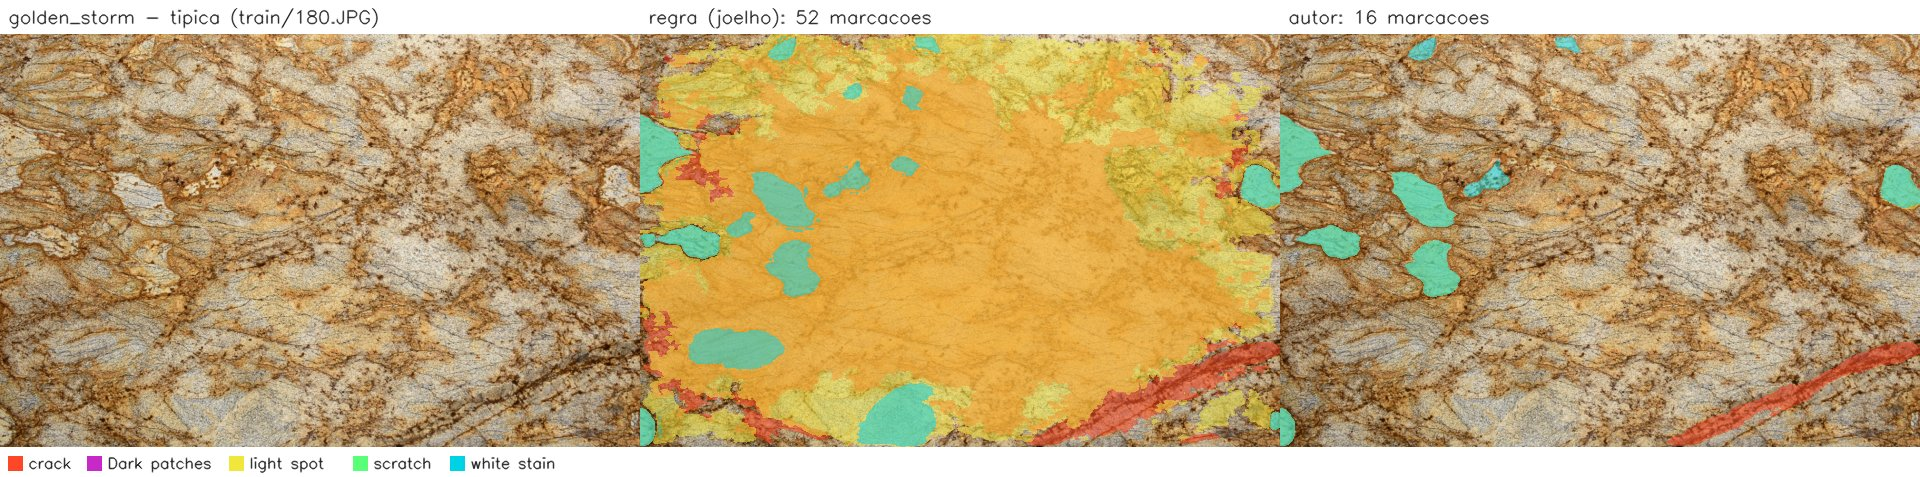
\includegraphics[width=\textwidth]{exemplo_golden_storm_tipica.jpg}

  \vspace{0.4cm}
  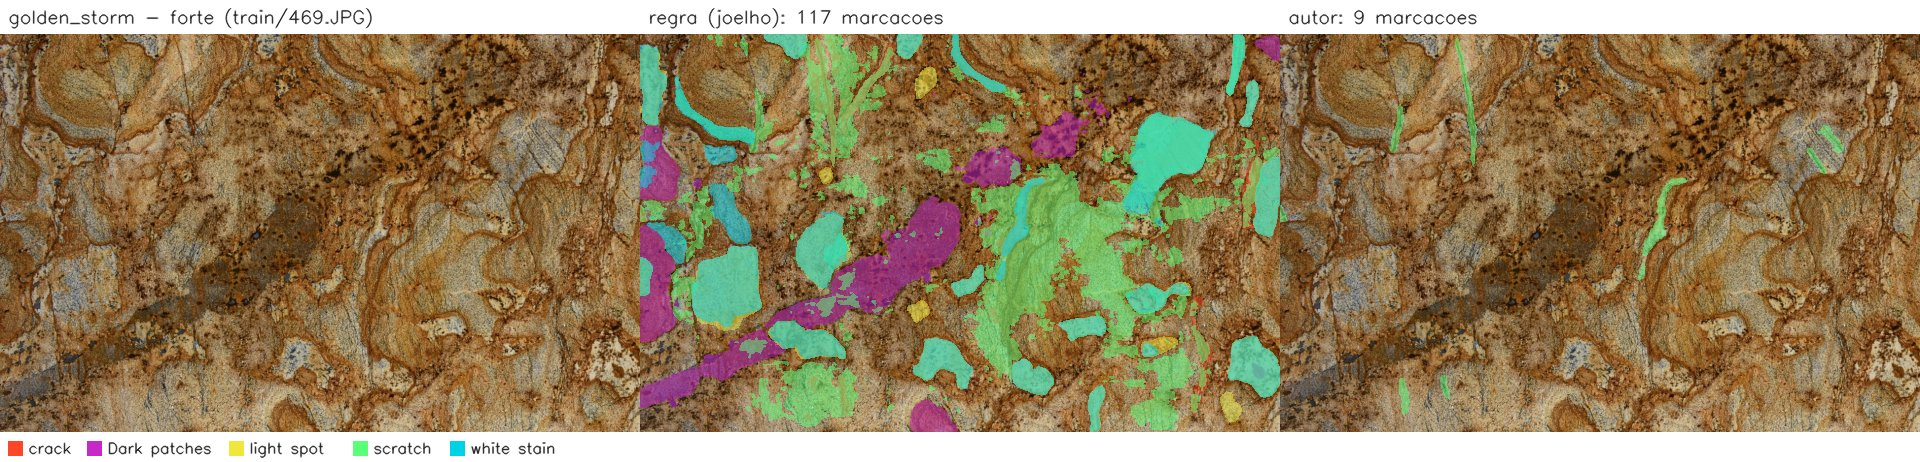
\includegraphics[width=\textwidth]{exemplo_golden_storm_forte.jpg}
  \legend{elaborado pelo autor, sobre imagens de \citeonline{dataset_araujo2023}}
\end{figure}

\begin{figure}[htbp]
  \caption{Regra e autor na \textit{ipanema\_beige}: imagem típica (acima) e forte (abaixo).}
  \label{fig:ex_ap_ipanema_beige}
  \centering
  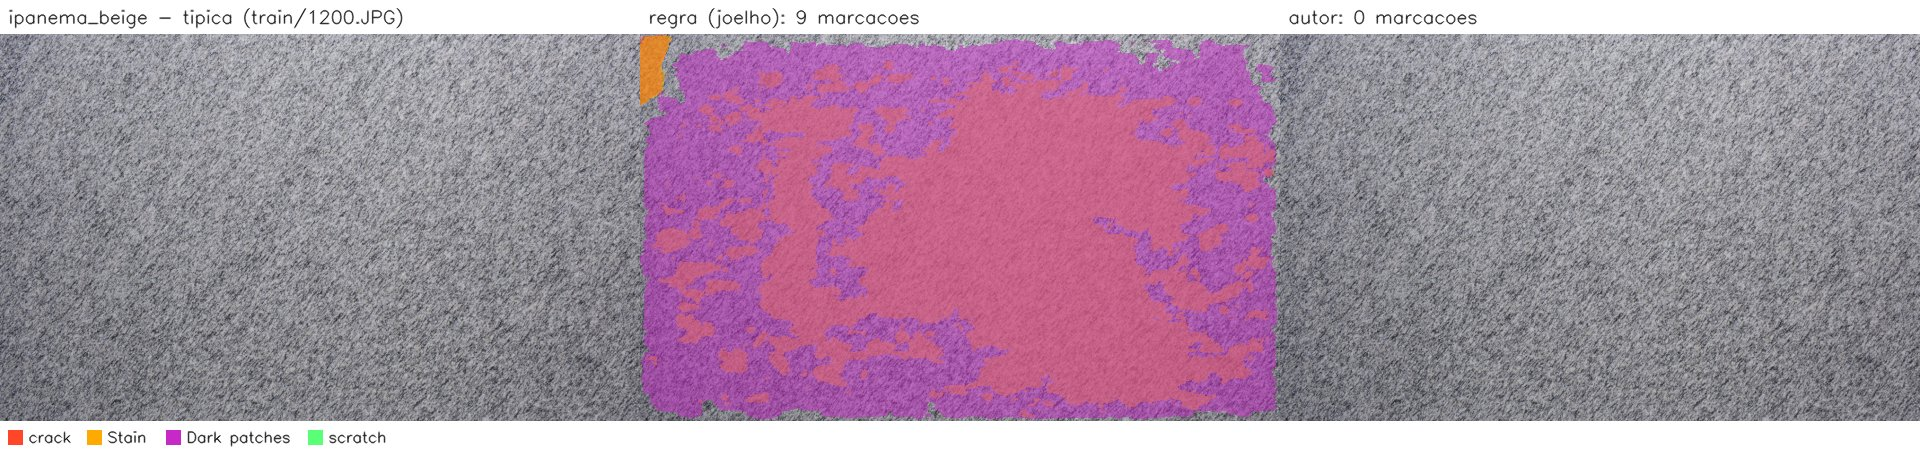
\includegraphics[width=\textwidth]{exemplo_ipanema_beige_tipica.jpg}

  \vspace{0.4cm}
  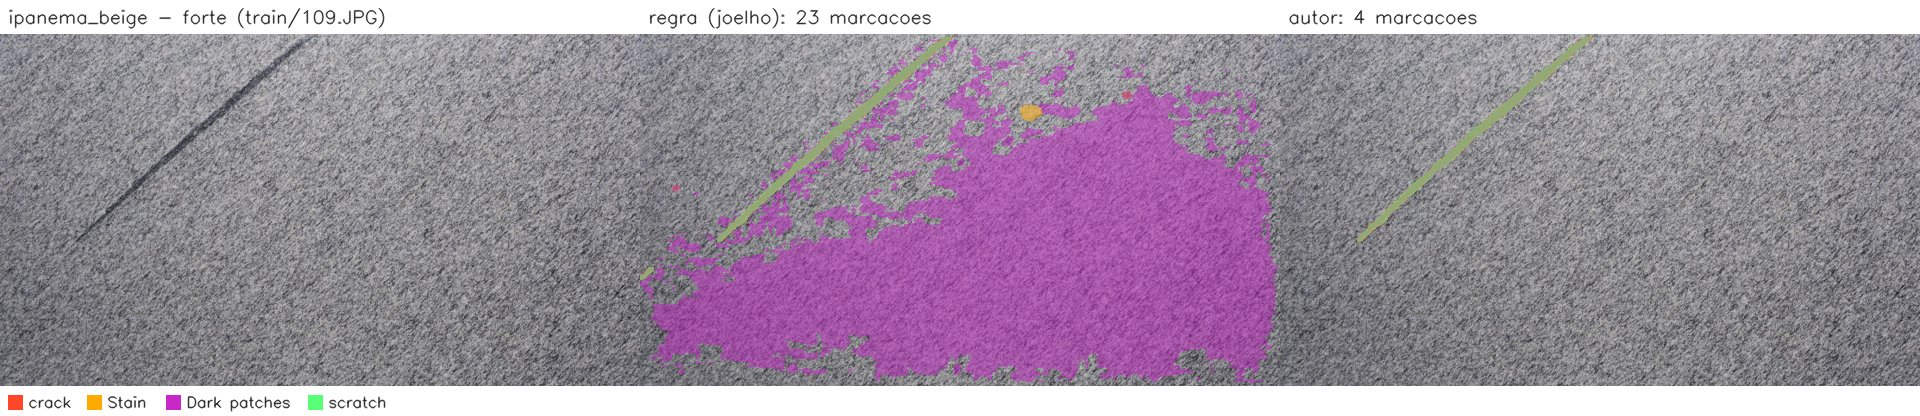
\includegraphics[width=\textwidth]{exemplo_ipanema_beige_forte.jpg}
  \legend{elaborado pelo autor, sobre imagens de \citeonline{dataset_araujo2023}}
\end{figure}

\begin{figure}[htbp]
  \caption{Regra e autor na \textit{itaunas\_white}: imagem típica (acima) e forte (abaixo).}
  \label{fig:ex_ap_itaunas_white}
  \centering
  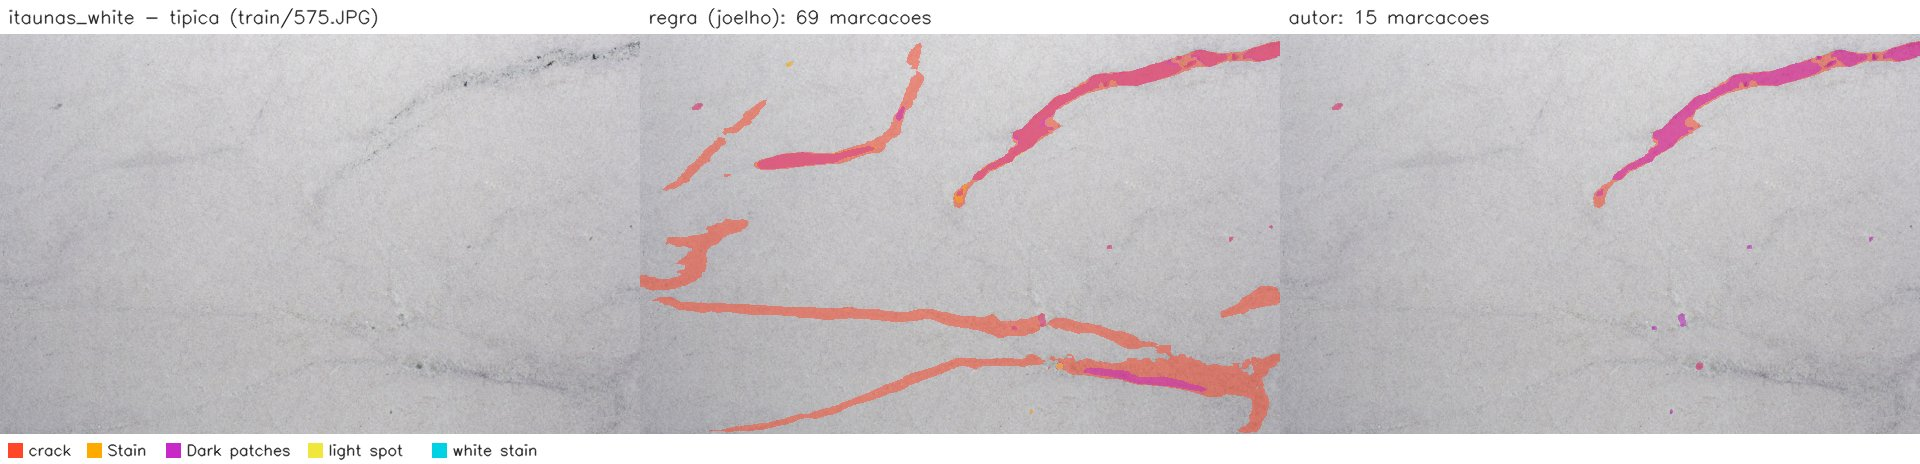
\includegraphics[width=\textwidth]{exemplo_itaunas_white_tipica.jpg}

  \vspace{0.4cm}
  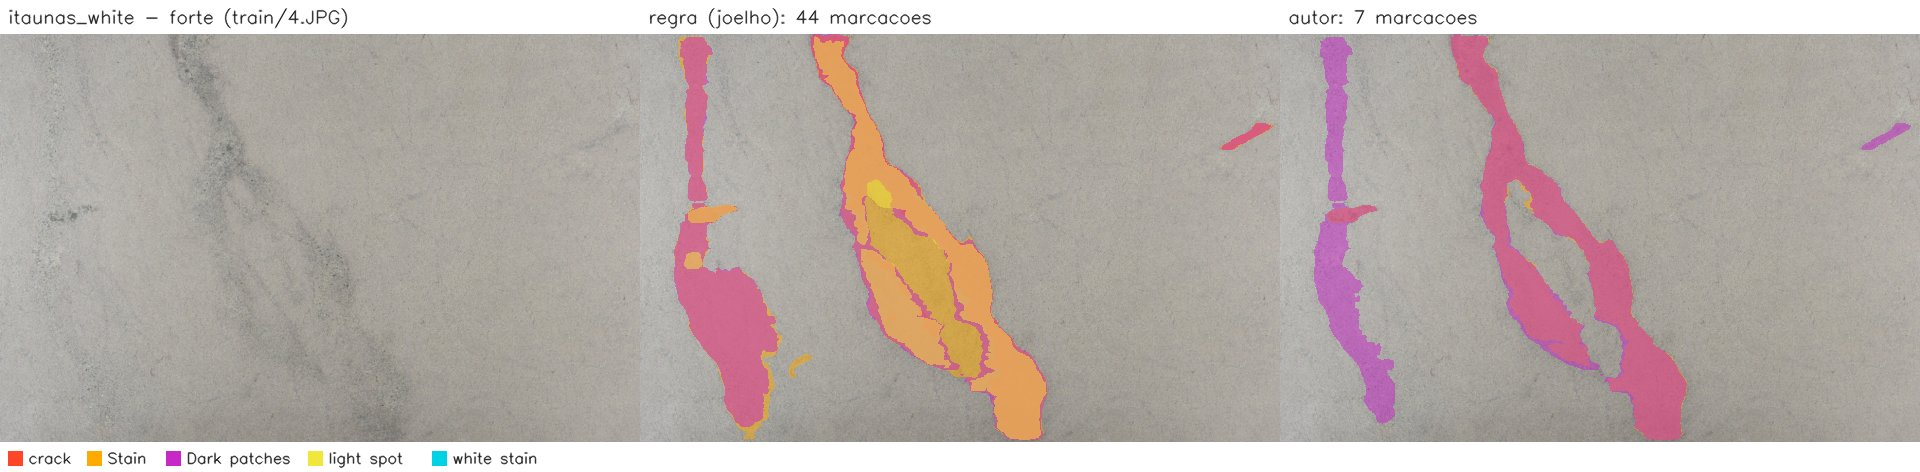
\includegraphics[width=\textwidth]{exemplo_itaunas_white_forte.jpg}
  \legend{elaborado pelo autor, sobre imagens de \citeonline{dataset_araujo2023}}
\end{figure}

\begin{figure}[htbp]
  \caption{Regra e autor na \textit{nevada\_black}: imagem típica (acima) e forte (abaixo).}
  \label{fig:ex_ap_nevada_black}
  \centering
  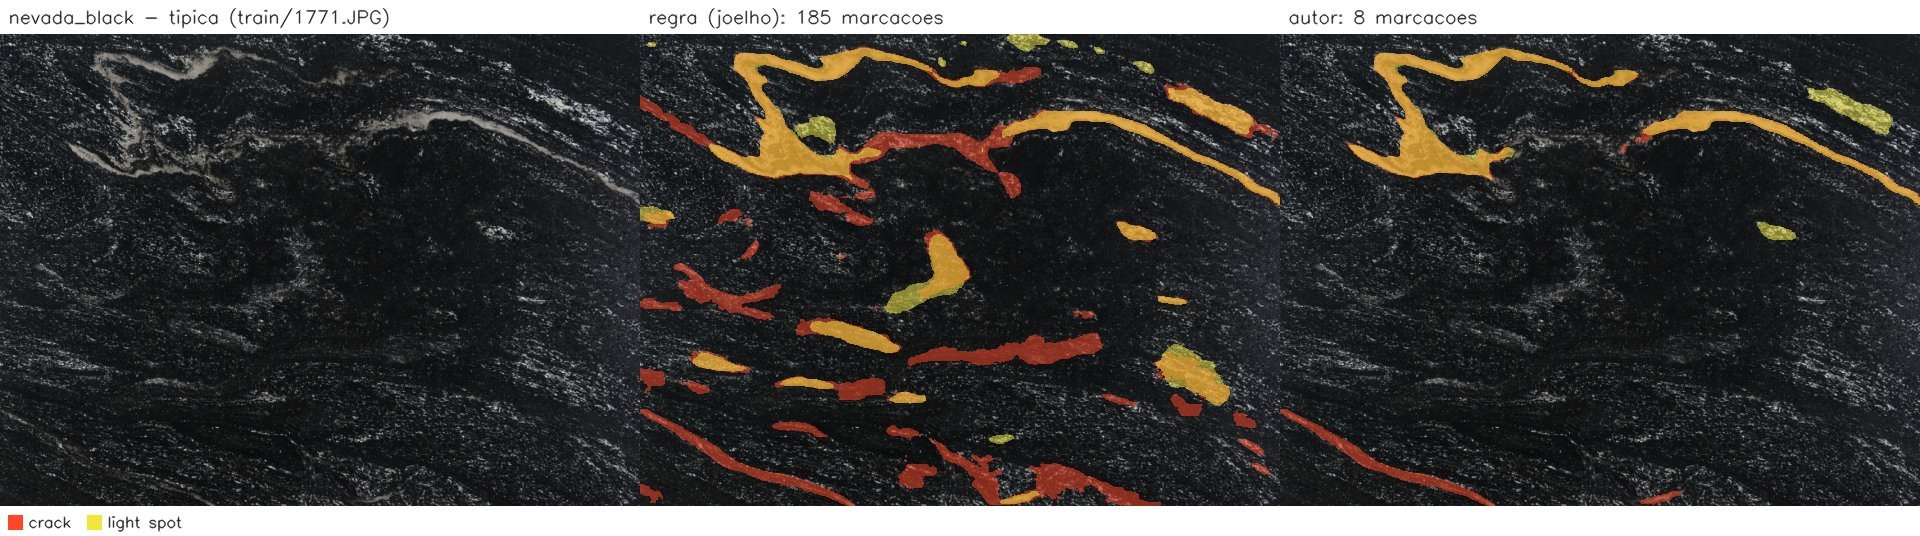
\includegraphics[width=\textwidth]{exemplo_nevada_black_tipica.jpg}

  \vspace{0.4cm}
  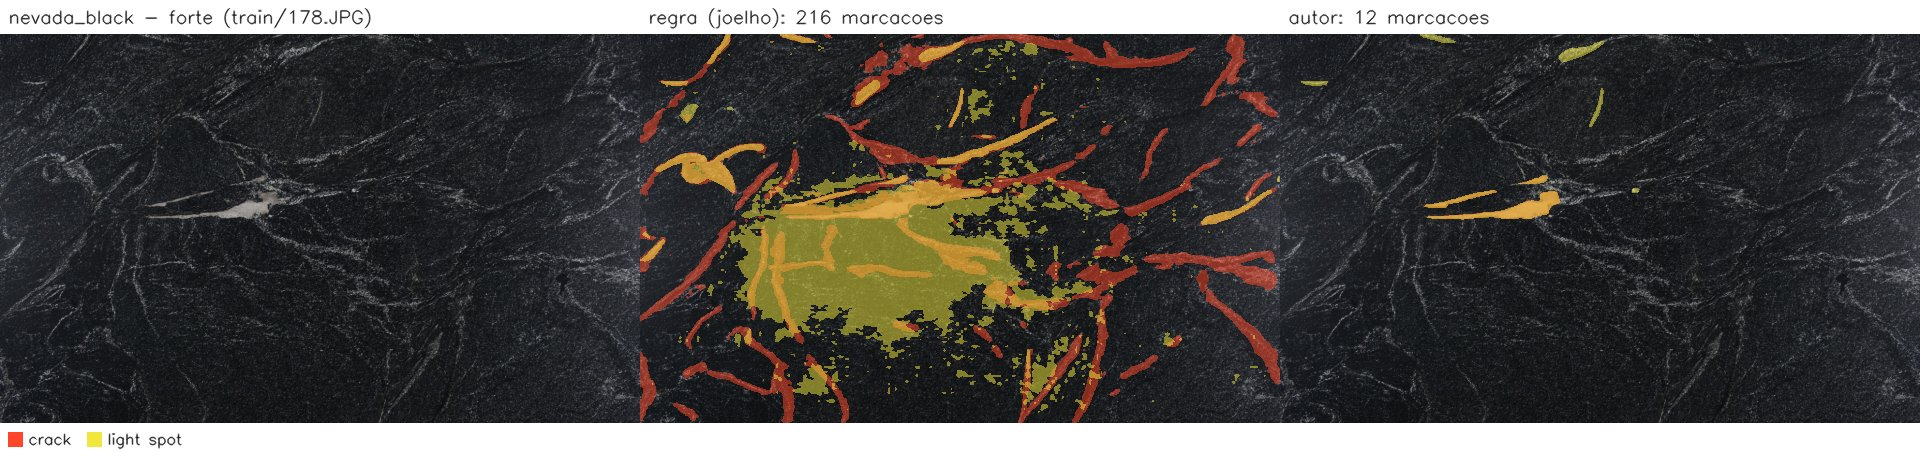
\includegraphics[width=\textwidth]{exemplo_nevada_black_forte.jpg}
  \legend{elaborado pelo autor, sobre imagens de \citeonline{dataset_araujo2023}}
\end{figure}

\begin{figure}[htbp]
  \caption{Regra e autor na \textit{san\_francisco\_green}$^{\dagger}$: imagem típica (acima) e forte (abaixo).}
  \label{fig:ex_ap_san_francisco_green}
  \centering
  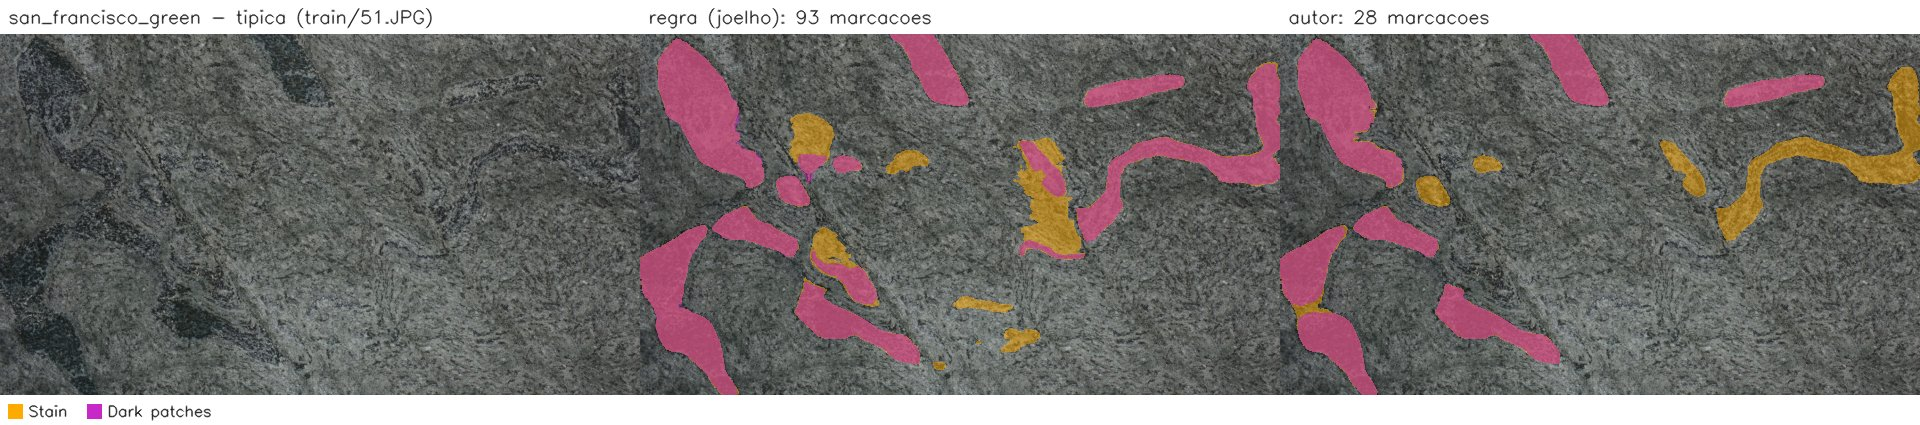
\includegraphics[width=\textwidth]{exemplo_san_francisco_green_tipica.jpg}

  \vspace{0.4cm}
  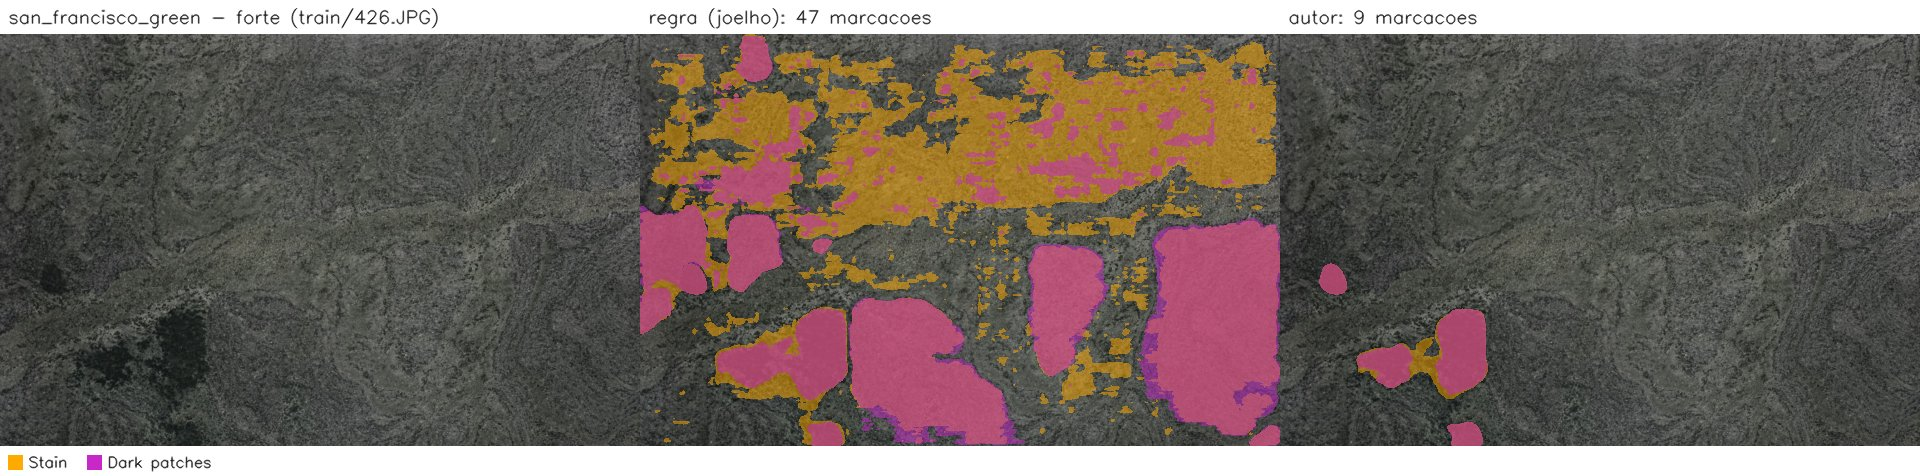
\includegraphics[width=\textwidth]{exemplo_san_francisco_green_forte.jpg}
  \legend{elaborado pelo autor, sobre imagens de \citeonline{dataset_araujo2023}}
\end{figure}

\begin{figure}[htbp]
  \caption{Regra e autor na \textit{santa\_cecilia}: imagem típica (acima) e forte (abaixo).}
  \label{fig:ex_ap_santa_cecilia}
  \centering
  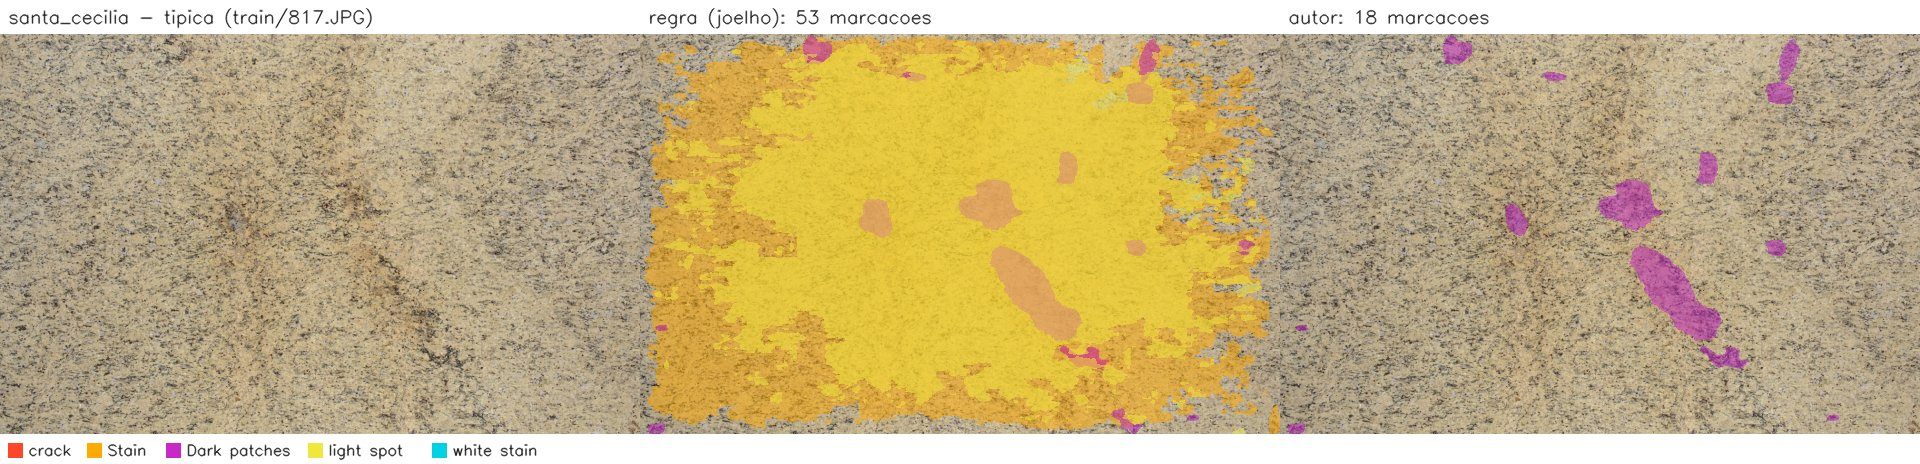
\includegraphics[width=\textwidth]{exemplo_santa_cecilia_tipica.jpg}

  \vspace{0.4cm}
  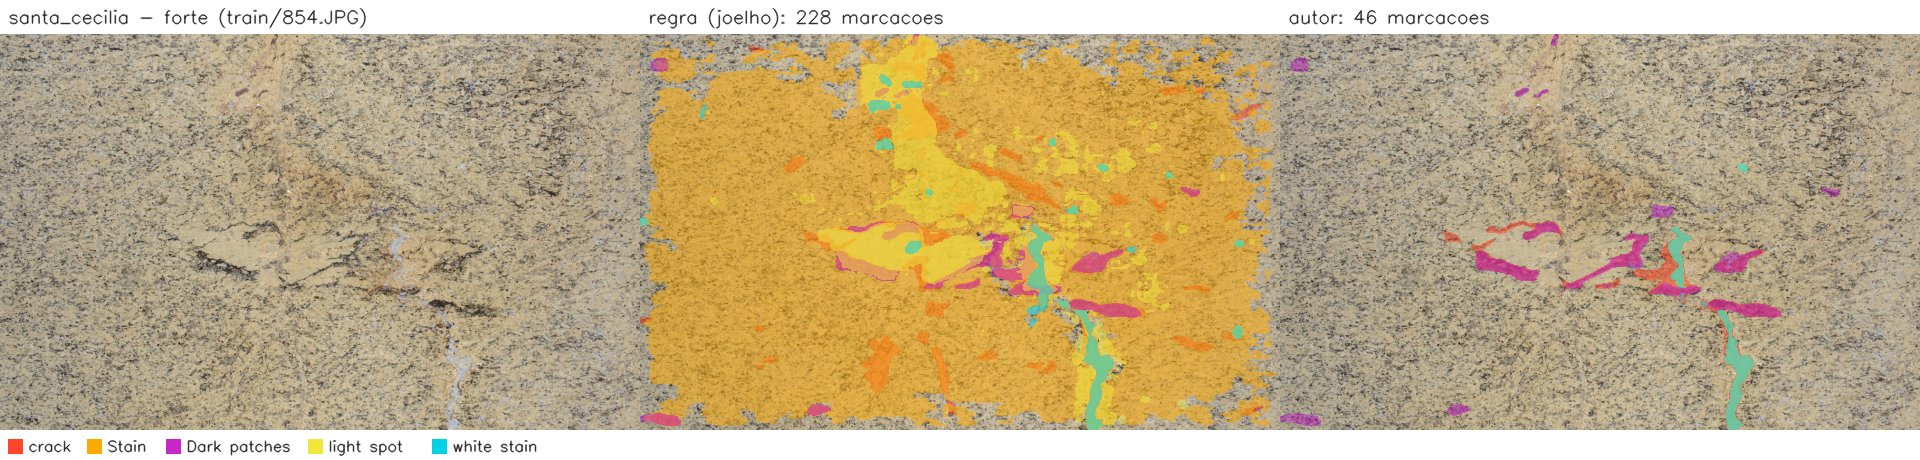
\includegraphics[width=\textwidth]{exemplo_santa_cecilia_forte.jpg}
  \legend{elaborado pelo autor, sobre imagens de \citeonline{dataset_araujo2023}}
\end{figure}

\begin{figure}[htbp]
  \caption{Regra e autor na \textit{shadow\_white}$^{\dagger}$: imagem típica (acima) e forte (abaixo).}
  \label{fig:ex_ap_shadow_white}
  \centering
  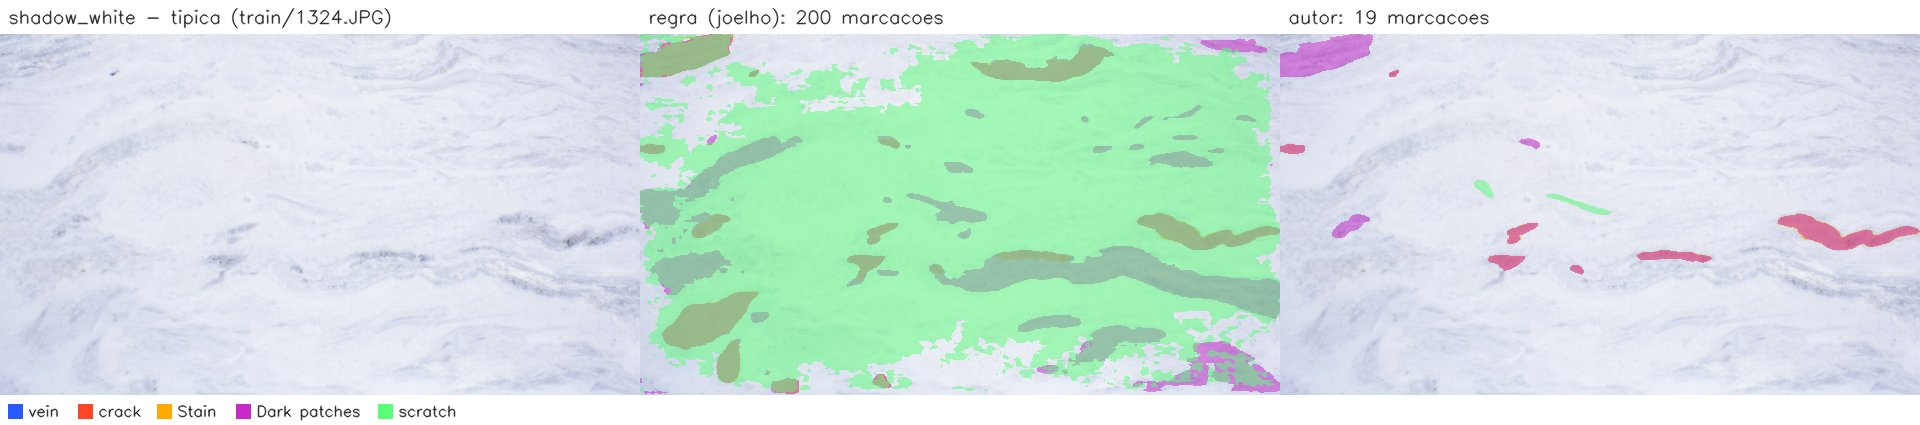
\includegraphics[width=\textwidth]{exemplo_shadow_white_tipica.jpg}

  \vspace{0.4cm}
  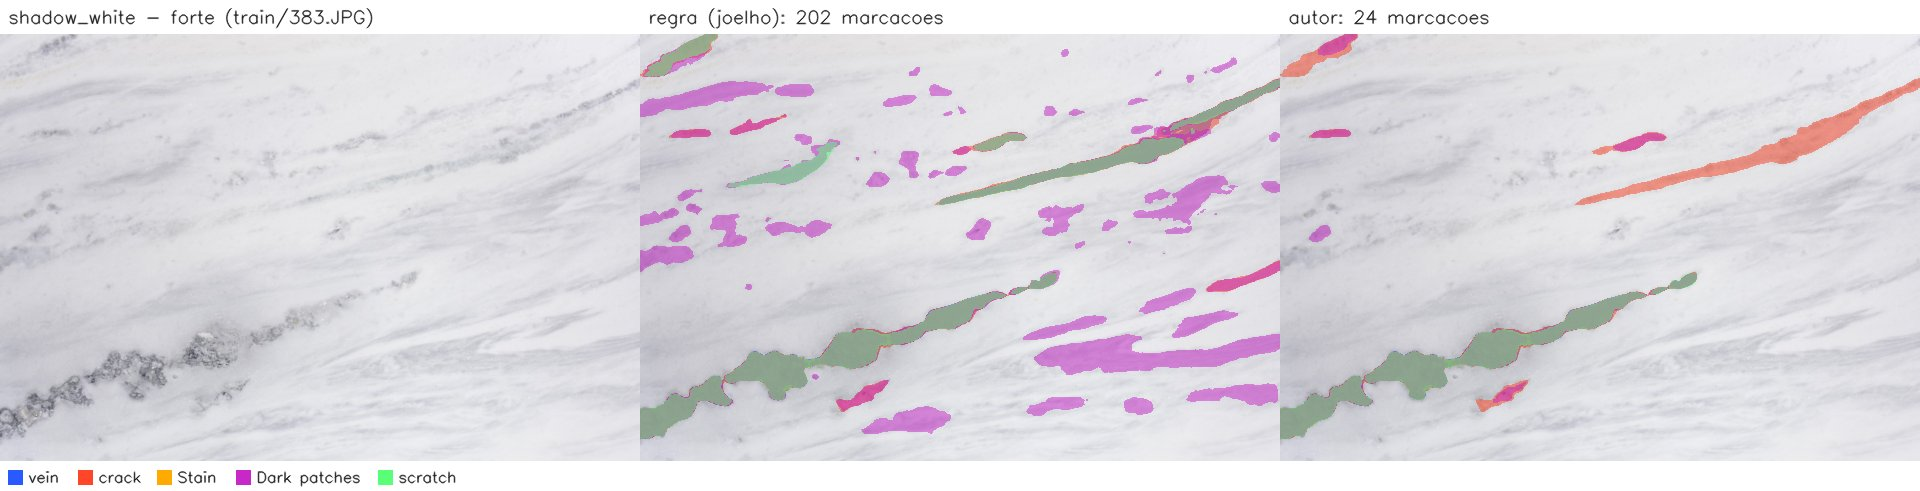
\includegraphics[width=\textwidth]{exemplo_shadow_white_forte.jpg}
  \legend{elaborado pelo autor, sobre imagens de \citeonline{dataset_araujo2023}}
\end{figure}

\begin{figure}[htbp]
  \caption{Regra e autor na \textit{siena\_white}: imagem típica (acima) e forte (abaixo).}
  \label{fig:ex_ap_siena_white}
  \centering
  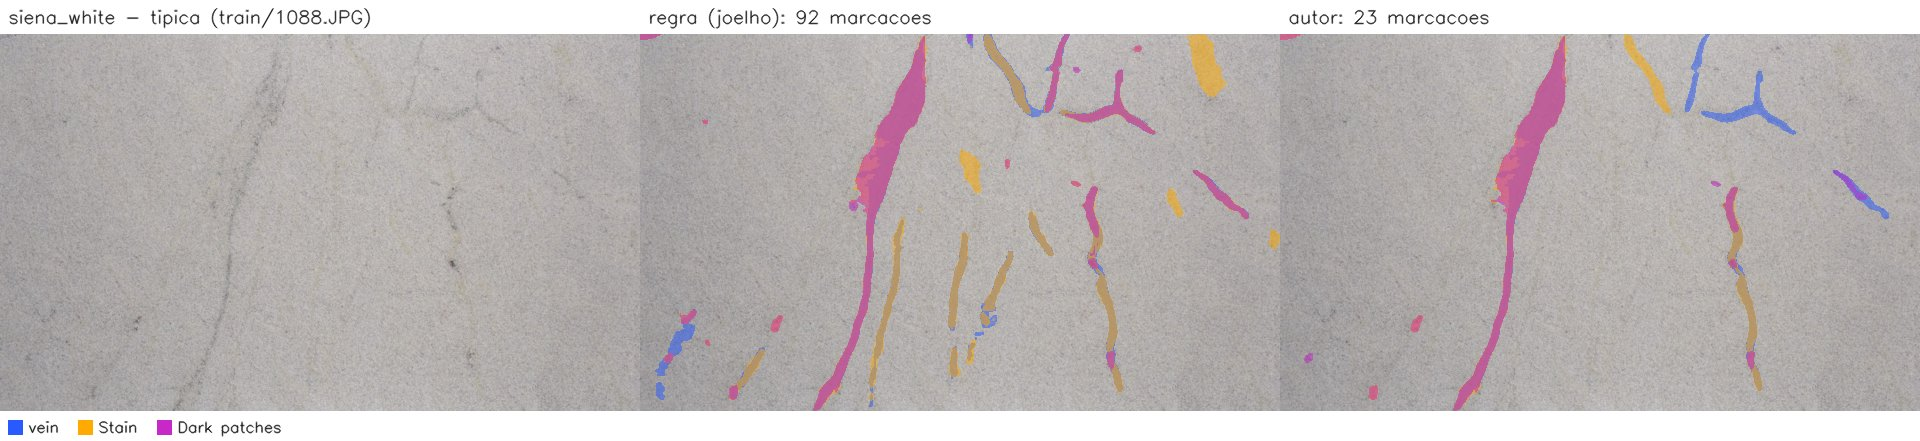
\includegraphics[width=\textwidth]{exemplo_siena_white_tipica.jpg}

  \vspace{0.4cm}
  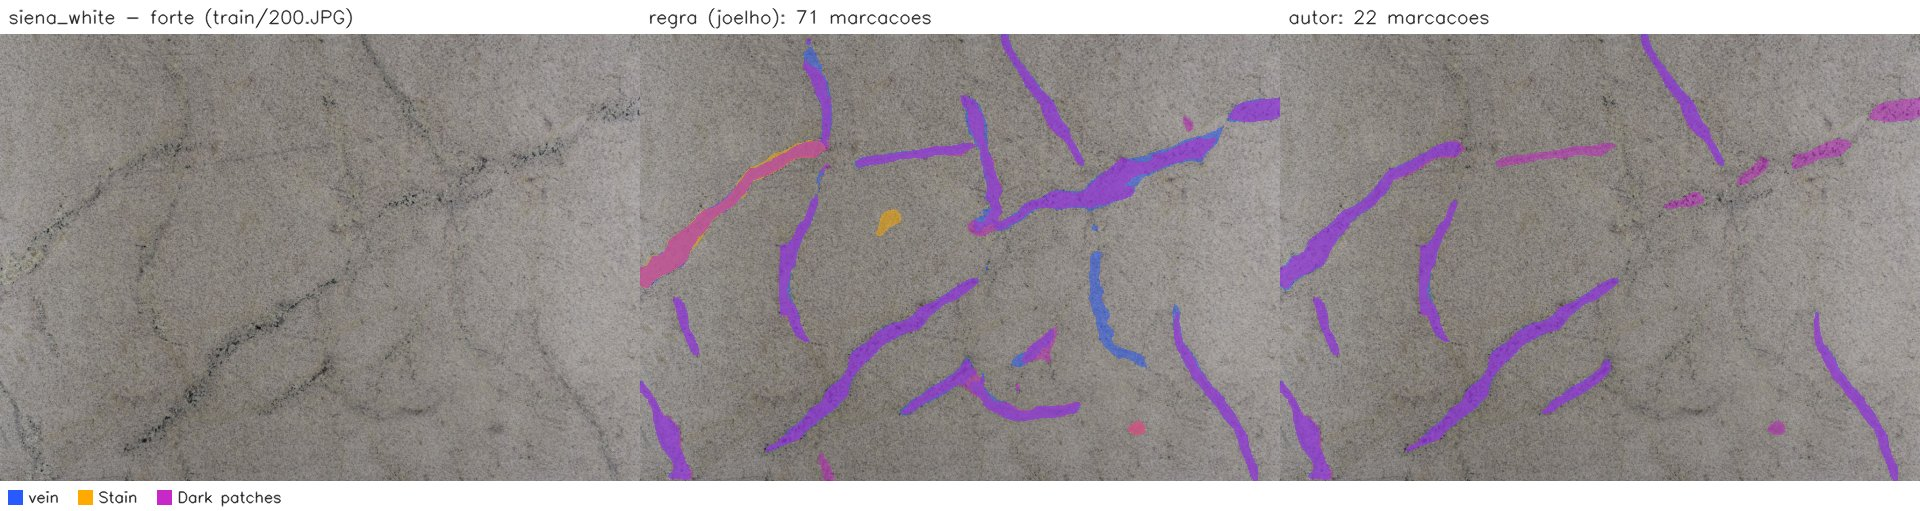
\includegraphics[width=\textwidth]{exemplo_siena_white_forte.jpg}
  \legend{elaborado pelo autor, sobre imagens de \citeonline{dataset_araujo2023}}
\end{figure}

\begin{figure}[htbp]
  \caption{Regra e autor na \textit{ubatuba\_green}: imagem típica (acima) e forte (abaixo).}
  \label{fig:ex_ap_ubatuba_green}
  \centering
  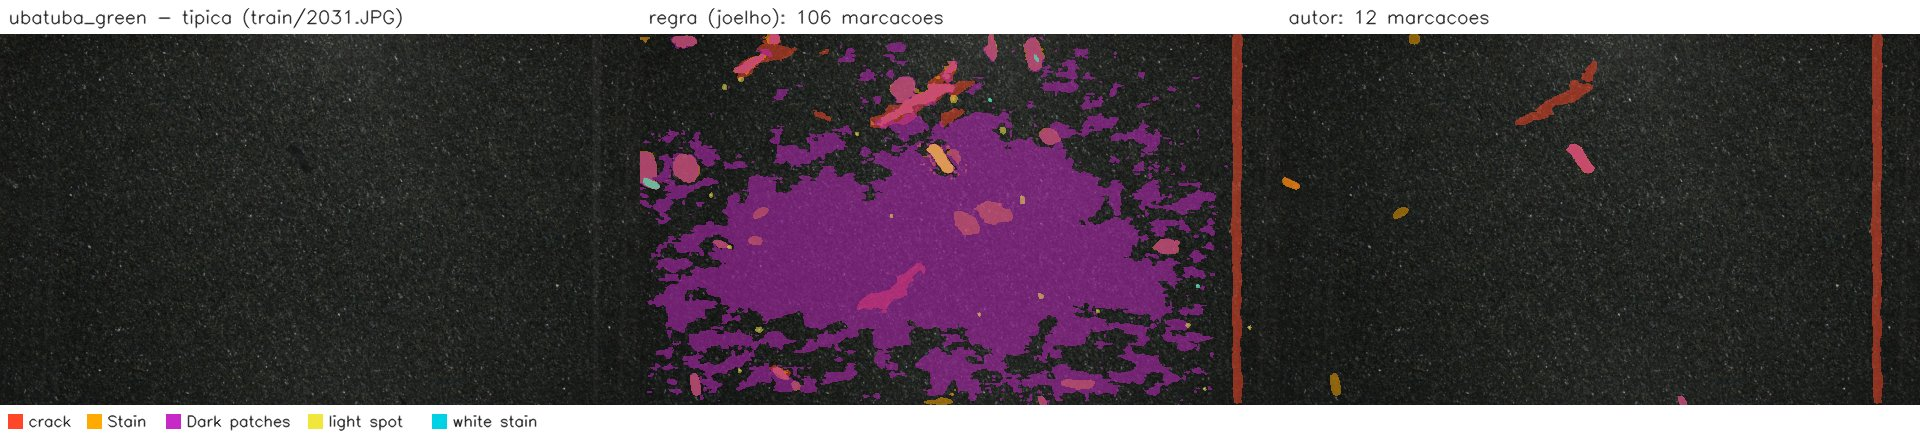
\includegraphics[width=\textwidth]{exemplo_ubatuba_green_tipica.jpg}

  \vspace{0.4cm}
  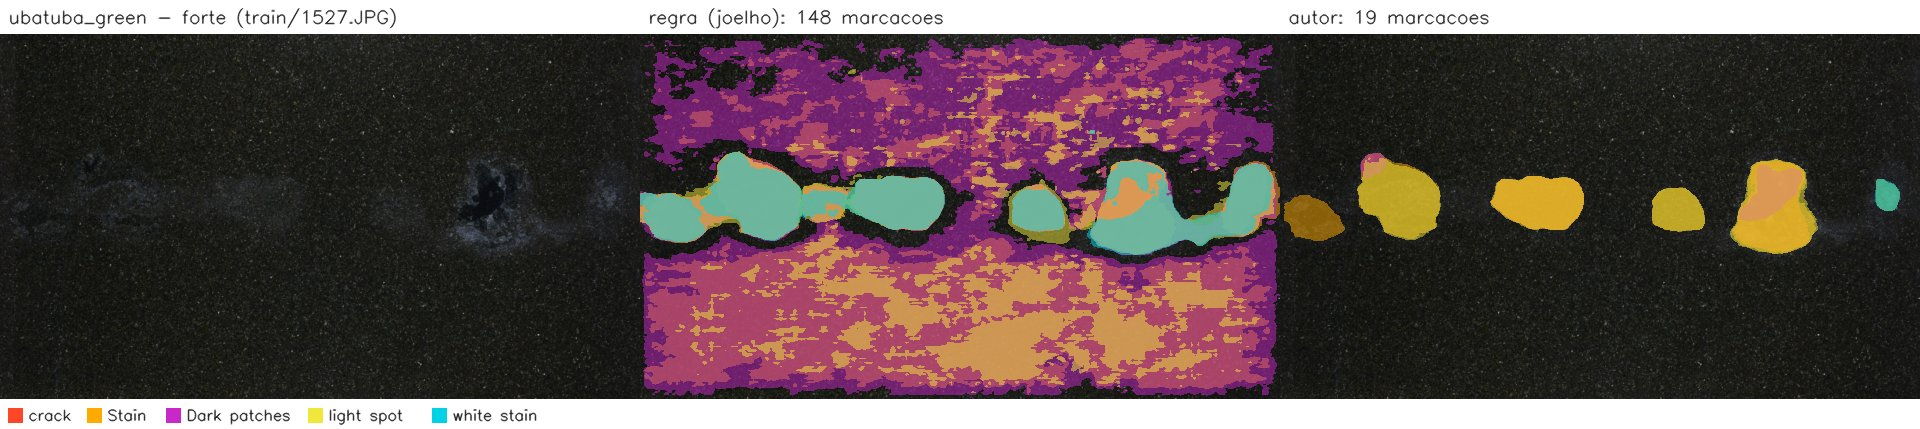
\includegraphics[width=\textwidth]{exemplo_ubatuba_green_forte.jpg}
  \legend{elaborado pelo autor, sobre imagens de \citeonline{dataset_araujo2023}}
\end{figure}

\begin{figure}[htbp]
  \caption{Regra e autor na \textit{white\_mirage}$^{\dagger}$: imagem típica (acima) e forte (abaixo).}
  \label{fig:ex_ap_white_mirage}
  \centering
  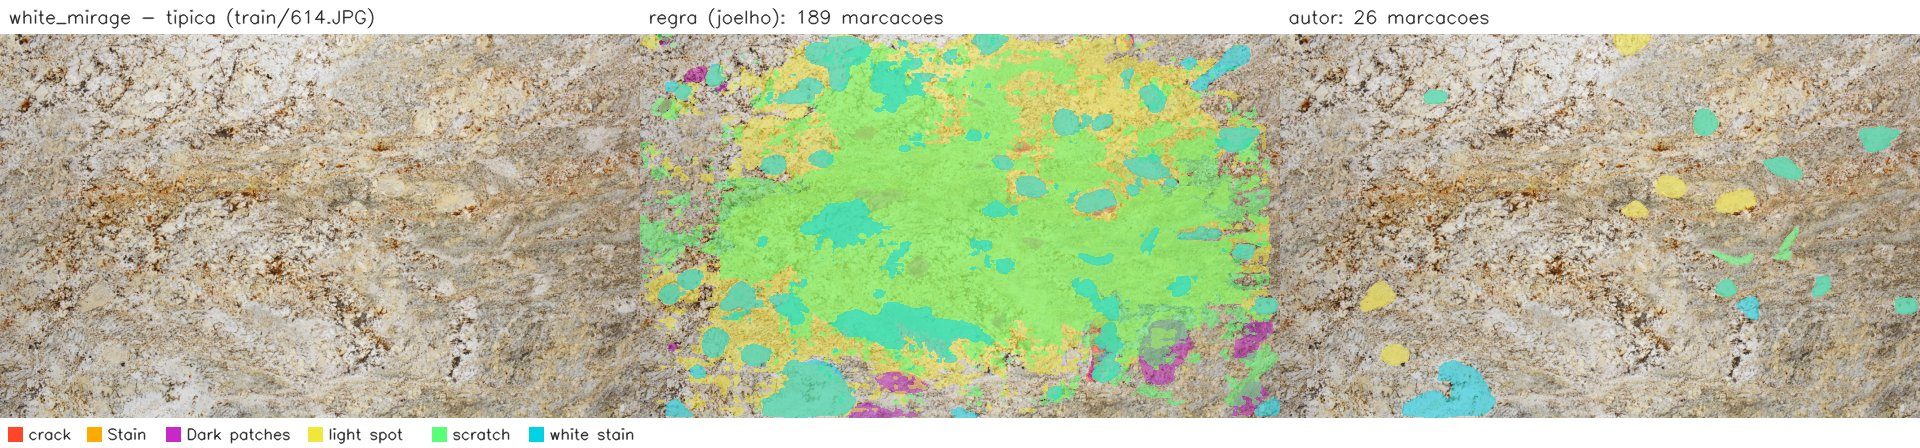
\includegraphics[width=\textwidth]{exemplo_white_mirage_tipica.jpg}

  \vspace{0.4cm}
  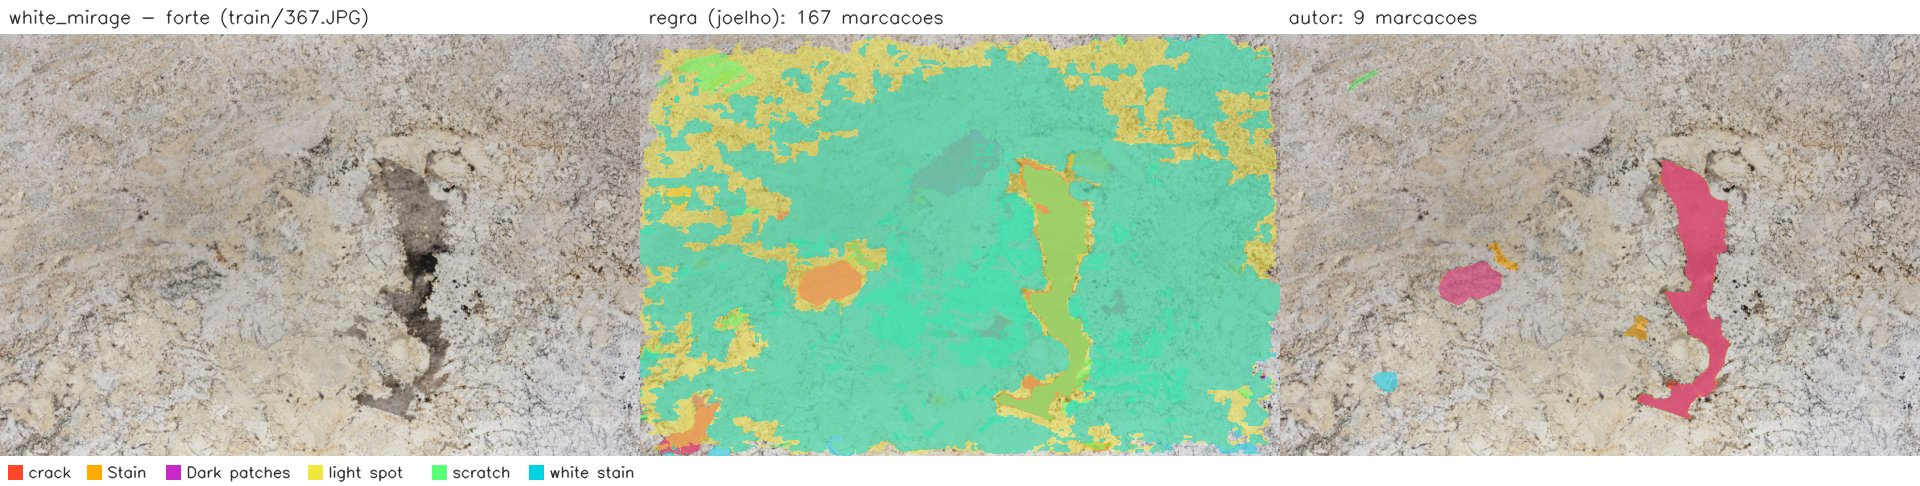
\includegraphics[width=\textwidth]{exemplo_white_mirage_forte.jpg}
  \legend{elaborado pelo autor, sobre imagens de \citeonline{dataset_araujo2023}}
\end{figure}

\begin{figure}[htbp]
  \caption{Regra e autor na \textit{white\_olympus}: imagem típica (acima) e forte (abaixo).}
  \label{fig:ex_ap_white_olympus}
  \centering
  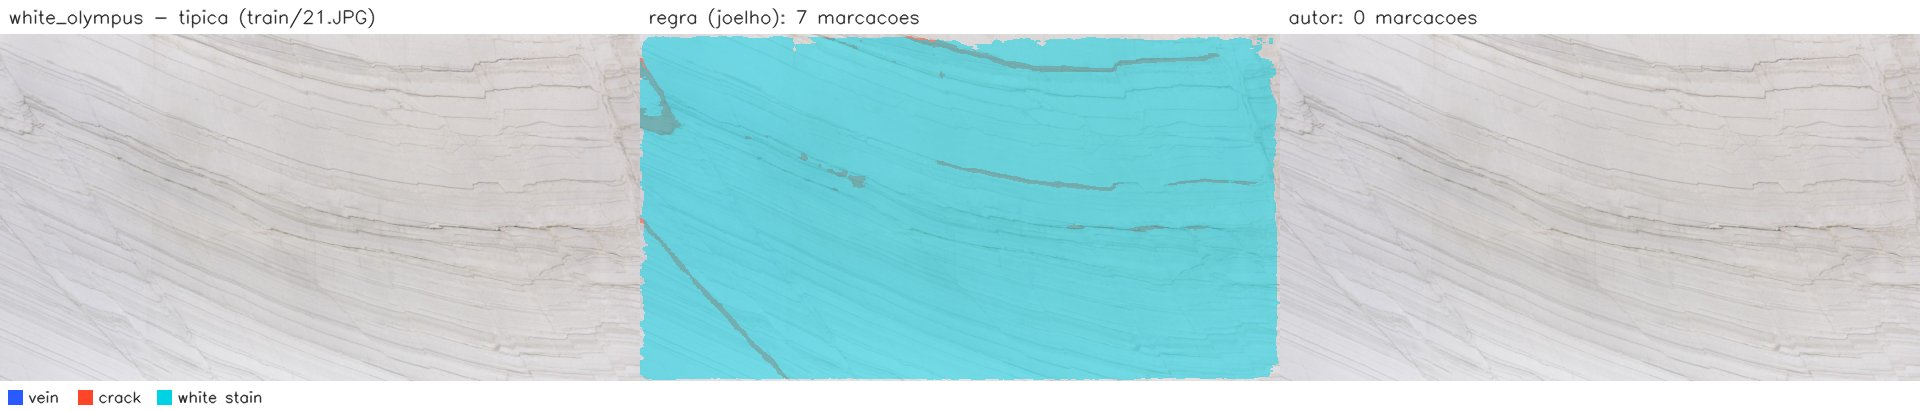
\includegraphics[width=\textwidth]{exemplo_white_olympus_tipica.jpg}

  \vspace{0.4cm}
  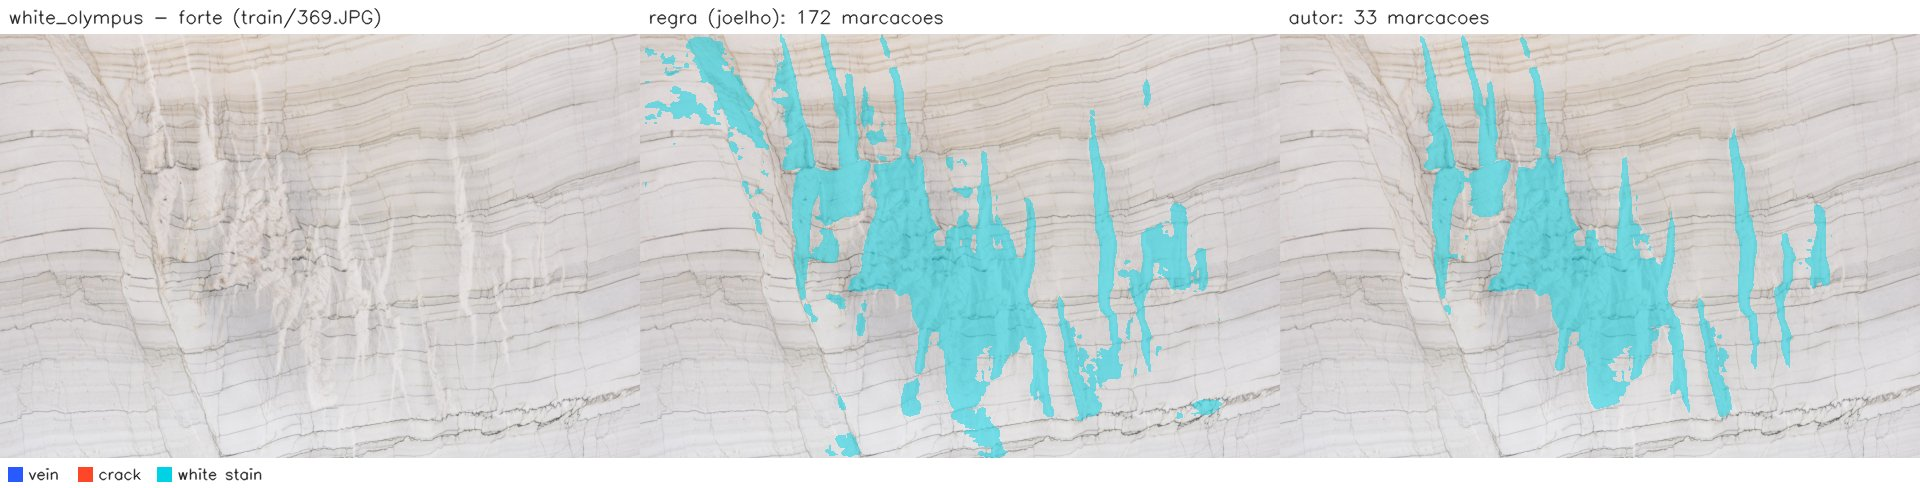
\includegraphics[width=\textwidth]{exemplo_white_olympus_forte.jpg}
  \legend{elaborado pelo autor, sobre imagens de \citeonline{dataset_araujo2023}}
\end{figure}

  \end{apendicesenv}

  % Anexos
  \begin{anexosenv}
    %%%\chapter{{\normalfont Explicação}}
\label{anexo: a}

É um elemento opcional. Não é elaborado pelo próprio autor mas sim por outras pessoas e constitui-se de suportes elucidativos e ilustrativos importantes para a compreensão do texto (ASSOCIAÇÃO BRASILEIRA DE NORMAS TÉCNICAS, 2011b). Havendo mais de um anexo, sua identificação deve ser feita por letra maiúscula ou algarismo arábico (ex:ANEXO A, ANEXO B), identificado por letras maiúsculas consecutivas,travessão e pelo respectivo título. 
    %%%\chapter{{\normalfont EasyReview}}

\lstset{
		keywordstyle=\bfseries\color{purple!60!black},
		commentstyle=\itshape\color{green!40!black},
% 		identifierstyle=\itshape,
		stringstyle=\itshape,
		showstringspaces=false,
		escapeinside={\%*}{*)},
		columns=flexible,
		breaklines=true,
breakindent=0pt}

\renewcommand\lstlistingname{Example}
\newcommand{\keyword}[1]{\textbf{\color{purple!60!black}{#1}}}

% ------
\textbf{\uppercase {The alert command}}

% ------
Command intended to claim author's attention to a given part of the text. In the following, it is possible to see an example:

\begin{center}
\begin{minipage}[ht]{0.45\textwidth}
\begin{lstlisting}[language=tex]
A text without the alert command. %*\keyword{$\backslash$alert}*){A text with the alert command}.
\end{lstlisting}
\end{minipage}
\hspace{10pt}
\begin{minipage}[ht]{0.45\textwidth}
A text without the alert command. \alert{A text with the alert command}.
\end{minipage}
\end{center}

% ------
\textbf{\uppercase {The highlight command}}

% ------
Command intended to claim author's attention to a given part of the text in a different to the ``alert'' command. In the following, it is possible to see an example:

\begin{center}
\begin{minipage}[ht]{0.45\textwidth}
\begin{lstlisting}[language=tex]
A text without the highlight command. %*\keyword{$\backslash$highlight}*){A text with the highlight command}.
\end{lstlisting}
\end{minipage}
\hspace{10pt}
\begin{minipage}[ht]{0.45\textwidth}
A text without the highlight command. \highlight{A text with the highlight command}.
\end{minipage}
\end{center}

% ------
\textbf{\uppercase {The remove command}}

% ------
Command which an author suggest to remove a given part of the text. In the following, it is possible to see an example:

\begin{center}
\begin{minipage}[ht]{0.45\textwidth}
\begin{lstlisting}[language=tex]
This text is not to be removed. %*\keyword{$\backslash$remove}*){This text is to be removed}.
\end{lstlisting}
\end{minipage}
\hspace{10pt}
\begin{minipage}[ht]{0.45\textwidth}
This text is not to be removed. \remove{This text is to be removed}.
\end{minipage}
\end{center}

% ------
\textbf{\uppercase {The add command}}

% ------
Command which an author suggest to add new text in a given part of the text. In the following, it is possible to see an example:

\begin{center}
\begin{minipage}[ht]{0.45\textwidth}
\begin{lstlisting}[language=tex]
This text was already in the text. %*\keyword{$\backslash$add}*){This text is been added now}.
\end{lstlisting}
\end{minipage}
\hspace{10pt}
\begin{minipage}[ht]{0.45\textwidth}
This text was already in the text. \add{This text is been added now}.
\end{minipage}
\end{center}

% ------
\textbf{\uppercase {The replace/substitute command}}

% ------
Both commands are equivalent. It shall be used when an author suggest to replace a given part of the text for a newer one. In the following, it is possible to see an example:

\begin{center}
\begin{minipage}[ht]{0.45\textwidth}
\begin{lstlisting}[language=tex]
%*\keyword{$\backslash$replace}*){This part of the text needs to be replaced}{for this newer part of the text}.
\end{lstlisting}
\end{minipage}
\hspace{10pt}
\begin{minipage}[ht]{0.45\textwidth}
\replace{This part of the text needs to be replaced}{for this newer part of the text}.
\end{minipage}
\end{center}

% ------
\textbf{\uppercase {The commentreview command}}

% ------
Command intended to claim author's attention to a given part of the text, giving some comments to provide more information. In the following, it is possible to see an example:

\begin{center}
\begin{minipage}[ht]{0.45\textwidth}
\begin{lstlisting}[language=tex]
%*\keyword{$\backslash$commentreview}*){This text will receive a comment.}{This is the comment I have!}.
\end{lstlisting}
\end{minipage}
\hspace{10pt}
\begin{minipage}[ht]{0.45\textwidth}
\commentreview{This text will receive a comment.}{This is the comment I have!}.
\end{minipage}
\end{center}
  \end{anexosenv}

  % Índice Remissivo
  \phantompart
  \printindex

\end{document}